\documentclass[11pt]{article}
\pdftrailerid{}
\usepackage[T1]{fontenc}
\usepackage[utf8]{inputenc}
\usepackage{mathpazo}
\usepackage[margin=1in]{geometry}
\usepackage{amsmath,amssymb,amsthm,mathtools}
\usepackage{booktabs,array,graphicx,mathrsfs}
\usepackage[numbers,sort&compress]{natbib}
\usepackage{tikz}
\usetikzlibrary{arrows.meta,positioning,calc}
\usepackage{url}
\urlstyle{same}
\usepackage[unicode,colorlinks=true,linkcolor=blue,citecolor=blue,urlcolor=blue]{hyperref}
\hypersetup{pdftitle={The Euclidean plane is not five-colorable},pdfauthor={OpenAI},pdfsubject={The Hadwiger--Nelson problem, arbitrary colorings, spectral rigidity, and measurable geometric obstructions},pdflang={en}}
\providecommand{\doi}[1]{doi: \href{https://doi.org/#1}{\nolinkurl{#1}}}
\renewcommand{\bibsection}{\section*{\refname}\addcontentsline{toc}{section}{\refname}}
\newtheorem{theorem}{Theorem}[section]
\newtheorem{lemma}[theorem]{Lemma}
\newtheorem{proposition}[theorem]{Proposition}
\newtheorem{corollary}[theorem]{Corollary}
\theoremstyle{definition}
\newtheorem{definition}[theorem]{Definition}
\theoremstyle{remark}
\newtheorem{remark}[theorem]{Remark}
\numberwithin{equation}{section}
\newcommand{\C}{\mathbb C}
\newcommand{\R}{\mathbb R}
\newcommand{\Q}{\mathbb Q}
\newcommand{\Z}{\mathbb Z}
\newcommand{\N}{\mathbb N}
\newcommand{\T}{\mathbb T}
\newcommand{\ind}{\mathbf 1}
\newcommand{\norm}[1]{\lVert#1\rVert}
\newcommand{\abs}[1]{\lvert#1\rvert}
\DeclareMathOperator{\id}{id}
\DeclareMathOperator{\dist}{dist}
\DeclareMathOperator{\supp}{supp}
\allowdisplaybreaks[1]
\setlength{\emergencystretch}{1em}

\title{The Euclidean plane is not five-colorable}
\author{OpenAI}
\date{September 23, 2026}
\begin{document}
\maketitle
\begin{abstract}
We prove that every coloring of the Euclidean plane with five colors has a
monochromatic unit-distance pair, with no regularity assumption on the color
classes. Consequently, the chromatic number of the plane is either six or seven.
\end{abstract}
\section{Introduction}\label{sec:introduction}

A proper $k$-coloring of the Euclidean plane is a function
$c:\R^2\to\{1,\ldots,k\}$ such that $c(x)\ne c(y)$ whenever
$\norm{x-y}=1$. The Hadwiger--Nelson problem asks for the least such
$k$, denoted by $\chi(\R^2)$, with no regularity imposed on the color
classes. Equivalently, it asks for the chromatic number of the graph
whose vertices are all points of the plane and whose edges are the
unit-distance pairs. Edges in a finite drawing of this graph may cross.

The problem dates to Edward Nelson in 1950. Nelson obtained the lower
bound four, and John Isbell found the upper bound seven by a hexagonal
coloring; the historical record of these unpublished observations is
recounted by \citet[pp.~15--19]{Soifer2003History}. Hadwiger's published
formulation \citep{Hadwiger1961} asks for a covering by sets that avoid
unit distance and gives the bounds four and seven. The seven-point
construction of \citet{MoserMoser1961}, now called the Moser spindle,
gives a particularly small finite obstruction to three colors. We use
its two overlapping-triangle constraints again in the final step of our
proof and verify the required placement explicitly.

The lower bound remained four until \citet{deGrey2018} constructed a
finite unit-distance graph that is not four-colorable in 2018.
His corrected construction has 1,581 vertices. Subsequent work made
these finite obstructions smaller and their verification more accessible:
\citet{Heule2018} used satisfiability proofs and extraction of
unsatisfiable cores to obtain 553-vertex examples, and
\citet{Parts2020Minimization} obtained a 509-vertex graph.
\citet{ExooIsmailescu2020} gave an alternative proof of the lower bound five,
and Parts gave a human-verifiable proof \citep{Parts2020Human}.
These advances concern finite obstructions to four colors. The
compactness theorem of \citet[Theorem~1]{deBruijnErdos1951} says that a
graph is $k$-colorable, for fixed finite $k$, if and only if every finite
subgraph is $k$-colorable. Consequently an unrestricted lower bound can
also be established without first displaying a finite graph witnessing
it.

The problem with measurable color classes has a different history.
Write $\chi_m(\R^2)$ for the least number of colors when each class must
be Lebesgue measurable. \citet{Falconer1981} proved
$\chi_m(\R^2)\ge5$ using density points and rotations.
\citet{Payne2009} developed this method for translation-invariant
unit-distance subgraphs. In particular, the graph on all of $\R^2$
whose edges have rational unit displacement vectors is two-colorable,
while every measurable coloring requires at least five colors. Thus
measurable and unrestricted colorings cannot be identified merely
because their distance constraints look the same.

For colorings by regular regions, \citet{Woodall1973} studied
distance-avoiding closed covers and region decompositions. Townsend
corrected Woodall's argument for a six-color lower bound in the
planar-map setting, announcing the repair in 1981 and giving its details
in 2005 \citep{Townsend1981,Townsend2005}. More recently,
\citet{SokolovVoronov2025} proved a lower bound seven for polygonal
colorings in a locally finite map framework. Their interface argument
excludes both adjacent colors wherever distances to the interface take
values both below and above one. We derive corresponding exclusions
from weak measurable data, without assuming regular color boundaries.

We prove the following result, working throughout in ZFC.

\begin{theorem}\label{thm:main}
The Euclidean plane has no proper five-coloring, even when arbitrary
color classes are allowed. Consequently,
\[
  6\le \chi(\R^2)\le 7.
\]
\end{theorem}

The remaining alternatives six and seven are unresolved.\footnote{
The May 14, 2026 manuscript of \citet{Reed2026} announces
$\chi(\R^2)=7$ through a circle-density argument. Its proposed strict
bound of $\pi/3$ on the angular measure of a unit-independent subset
of the unit circle fails for the half-open arc
$\{e^{it}:0\le t<\pi/3\}$: this arc has angular measure $\pi/3$
and contains no unit pair. The displayed formal theorem assumes that
density bound as a hypothesis, so the argument does not establish the
announced equality.}
The proof has two parts: a transfer from unrestricted proper colorings to a
measurable condition, and a geometric obstruction to five labels under that condition.
The transfer holds for every finite number of colors.

\begin{definition}[Weak measurable coloring]\label{def:weak-coloring}
Let $k$ be a positive integer, let $S^1\subset\R^2$ be the unit circle,
and let $\sigma$ be its normalized arc-length measure. A
\emph{weak measurable $k$-coloring} is a Lebesgue measurable function
$c:\R^2\to\{1,\ldots,k\}$, with color classes $A_i=c^{-1}(\{i\})$,
such that, for every $R>0$,
\[
  \sum_{i=1}^k\int_{B(0,R)}\int_{S^1}
  \ind_{A_i}(x)\ind_{A_i}(x+u)\,d\sigma(u)\,dx=0.
\]
The integrals use the completed product measure; equivalently, one
may first choose Borel representatives of the color classes forming
a partition of the plane.
\end{definition}

This definition permits exceptional unit pairs. It is unchanged by
modifying the coloring on a plane Lebesgue null set: by Fubini, the
pairs for which either $x$ or $x+u$ belongs to that set have product
measure zero. The required bridge to the unrestricted problem is the
following equivalence.

\begin{theorem}[Transfer of colorability]\label{thm:transfer}
For every positive integer $k$, in ZFC,
\begin{equation}\label{eq:source-1}
  \begin{gathered}
    \text{a proper $k$-coloring of $\R^2$ exists}
    \\ \Longleftrightarrow \\
    \text{a weak measurable $k$-coloring of $\R^2$ exists}.
  \end{gathered}
\end{equation}
\end{theorem}

\begin{theorem}\label{thm:weak-five}
There is no weak measurable five-coloring of the Euclidean plane.
\end{theorem}

\begin{proof}[Deduction of Theorem~\ref{thm:main}]
A proper five-coloring would give a weak measurable five-coloring by
Theorem~\ref{thm:transfer}, contrary to Theorem~\ref{thm:weak-five}.

For the upper bound, use the hexagonal construction described by
\citet{Hadwiger1961}.
Take Voronoi hexagons of a triangular lattice, each with circumradius
$r=2/5$. Their centers have nearest-neighbor distance $\sqrt3r$.
Write the lattice as a scaled copy of $\Z+\Z\omega$, where
$\omega=e^{2\pi i/3}$. Multiplication by $2-\omega$ gives a similar
sublattice of index seven, since $|2-\omega|^2=7$. Color centers by
its seven cosets, and give each point the color of its hexagon,
assigning boundary points to any incident hexagon. Distances inside
one hexagon are at most $2r<1$. Centers of distinct same-color
hexagons are at least $\sqrt{21}r$ apart, so points in those hexagons
are at least $(\sqrt{21}-2)r>1$ apart. This is a proper seven-coloring,
including all boundaries.
\end{proof}

\subsection{Proof overview and the role of earlier methods}

The two parts of the proof address different obstacles. A coloring with
arbitrary classes provides no density-point structure to use, while a measurable
coloring may have boundaries far too irregular to analyze as a planar
map. Theorem~\ref{thm:transfer} supplies the measurable input. The proof
of Theorem~\ref{thm:weak-five} then constructs the connected interfaces
it needs instead of assuming them. Figure~\ref{fig:proof-route} shows how
these two parts combine.

\paragraph{From arbitrary labels to measurable fields.}
Let $F$ be the field of real algebraic numbers, $E=F(i)$ the algebraic
plane, and $K=\{u\in E:|u|=1\}$ its group of algebraic rotations.
Restricting a proper coloring to the countable set $E$ and averaging
its translates and rotations gives an invariant probability law on
proper labelings of $E$. This is a standard amenable averaging
construction. Probabilistic approaches to the Hadwiger--Nelson problem
already use invariant randomization and finite-graph compactness
\citep{BourgeatHeinrichMelottiRobert2015,GwynStavrianos2020};
F\o lner averaging over countable groups of plane isometries also occurs
in the fractional-coloring work of
\citet{MatolcsiRuzsaVargaZsamboki2025}. These methods supply symmetry.
Here a further argument must retain the unit-distance exclusions while
producing ordinary measurable functions on the plane.

For this purpose let $D$ be the compact group of all characters of the
additive discrete group $E$. A character is a homomorphism from $E$ to
the unit complex circle. The ordinary continuous characters form the
Borel subgroup
\[
 C=\{z\mapsto\exp(i\xi\cdot z):\xi\in\R^2\}\subset D.
\]
Rotations act on characters by $(ud)(z)=d(uz)$.
The spectral theorem, in $L^2$ of the invariant labeling law,
separates each label indicator into the part
supported on $C$ and its orthogonal remainder. The central rigidity
statement, Theorem~\ref{thm:rigidity}, says that every $K$-invariant
probability on $D$ assigning zero mass to $C$ is Haar probability. The
remainder therefore has zero correlation under every nonzero algebraic
translation, so removing it preserves the zero unit correlations.
The $C$-supported subspace is the space of functions on a probability
factor, so projection onto it is conditional expectation and preserves
nonnegativity and keeps the sum of the label coordinates equal to one.
Translation operators on this factor extend continuously to $\R^2$.
The translated coordinates admit jointly measurable versions, giving
fields on the plane and the probability space. For a suitable sample,
choose the least label with positive coordinate at each point
where the coordinates sum to one, and assign arbitrary labels on the
remaining plane-null set. The zero unit correlations give the weak
measurable coloring condition. Section~\ref{sec:transfer} carries out this passage, including
the measurable-version and exceptional-pair details.

The rigidity proof occupies Sections~\ref{sec:spectral}
and~\ref{sec:rigidity}. Its structural ingredient is the
Furstenberg--Zimmer compact-extension method
\citep{Furstenberg1977,ZimmerExtensions1976,ZimmerDiscrete1976}.
We give the particular compact-factor tower and conditional averaging
arguments used here; the corrected modern account of
\citet{JamneshanStructure,JamneshanCorrigendum} supplies further
context. For an ergodic law, a relative singularity lemma along that
tower shows that the
law of the difference of two characters, sampled conditionally independently
over its terminal factor, still gives $C$ measure zero. Its Fourier
coefficient is nonnegative and radial, and its line averages defined
by an invariant mean vanish.
Two identities between sums of algebraic unit directions give a difference
inequality for this coefficient. A finite number-field argument shows
that a positive value at any nonzero radius would force a uniform positive
lower bound on an interval of algebraic radii, contradicting those averages.
This proves Haar rigidity without a regularity assumption on the original
coloring.

For the converse transfer, density points of a weak color class contain no unit pair
(Lemma~\ref{lem:palettes-density-proper}). This adapts the familiar
density-point mechanism of Falconer and Payne to product-almost-everywhere
unit-pair exclusion. A common
translation places any fixed finite configuration among points having
density one in their assigned color, called typical points,
and graph compactness then gives a proper coloring of the whole plane.
The weak condition uses Lebesgue measure in position and arc length in
direction; it is distinct from the invariant-mean notion of
monochromatic-pair frequency in \citet{GwynStavrianos2020}.

\paragraph{From weak labels to connected exclusions.}
For the five-color obstruction, fix a center $x$ and take weak-* limits
of the typical angular samples
$e\mapsto(\ind_{A_i}(y+re))_{i=1}^5$, where $e\in S^1$,
$y\to x$, and $r\to1$. The \emph{palette} at $(x,e)$ collects,
up to angular null sets, all labels having positive weight at $e$ in
these limits. Smooth transport of two unit directions gives exclusions
between palettes. Section~\ref{sec:palettes}
shows that almost every palette contains at most two labels, at every
fixed center. Section~\ref{sec:transitions} records abundant transitions
between labels in a finite graph at each center and proves that centers
where this graph contains a cycle form a closed locally finite set.
The estimates use the decay of the Fourier transform of circle measure;
no finite perimeter or smoothness of a color boundary is assumed.

Section~\ref{sec:interfaces} smooths the color indicators by disk
averages, then thresholds and renormalizes the resulting probability
vectors. Outside disks with vanishing total radii, these modified
vectors have at most two positive coordinates, so they lie in the
complete graph on the five labels. The forest
structure away from cyclic centers lets us fill the holes in those regions
continuously in that graph. A planar cover obstruction forces a
nontrivial loop around one cyclic-center disk. A simple cycle in the
reduced edge path of that loop supplies the label cycle. For each edge
midpoint, a connected component of its inverse image crosses the annulus.
Limits of these components give compact connected sets $K_j$ with a
common point $x$.
Each $K_j$ is assigned the two endpoint labels of its edge.
Both endpoint labels are absent almost everywhere from the open region
\[
 \Delta(K_j)=\{z:\min_{q\in K_j}|z-q|<1<\max_{q\in K_j}|z-q|\}.
\]
This connected-set exclusion has a geometric predecessor in the
interface arguments of \citet[Propositions~1--2]{SokolovVoronov2025}.
Here the continua and their common point are consequences of the
measure estimates and the topological extraction.

A simple cycle on five labels has length three, four, or five.
Section~\ref{sec:angular} excludes each possibility. Chosen limiting
directions of sequences in the continua approaching $x$ determine
allowed labels just inside and just outside the unit circle about $x$. A five-cycle gives
incompatible six-position angular words. A four-cycle gives two antipodal
pairs of directions and an impossible parity rule. A three-cycle forces six
alternating sectors for the two outside labels. The last configuration
leaves an open region using only the three cycle labels almost everywhere; a rational
placement certificate puts all seven vertices of the Moser obstruction
in that region. These contradictions complete the proof of
Theorem~\ref{thm:weak-five}.

\begin{figure}[htbp]
\centering
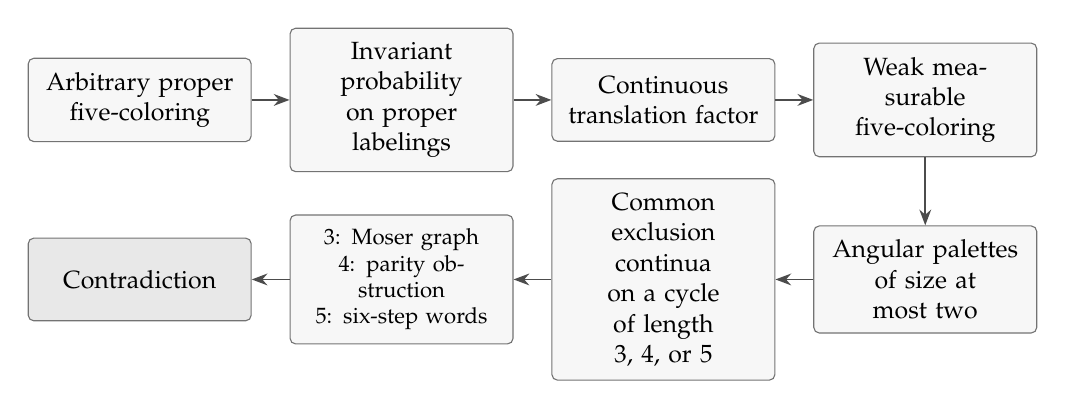
\begin{tikzpicture}[
  font=\small,
  stage/.style={draw=black!55, rounded corners=2pt, fill=black!3,
    align=center, text width=2.48cm, minimum height=1.05cm,
    inner sep=5pt},
  link/.style={-{Stealth[length=2mm]}, semithick, draw=black!70},
  node distance=0.48cm]
  \node[stage] (proper) {Arbitrary proper\\five-coloring};
  \node[stage, right=of proper] (law)
    {Invariant probability\\on proper labelings};
  \node[stage, right=of law] (factor)
    {Continuous\\translation factor};
  \node[stage, right=of factor] (weak)
    {Weak measurable\\five-coloring};
  \node[stage] (palettes) at ([yshift=-2.28cm]weak.center)
    {Angular palettes\\of size at most two};
  \node[stage] (cycle) at ([yshift=-2.28cm]factor.center)
    {Common exclusion\\continua on a cycle\\of length $3$, $4$, or $5$};
  \node[stage, text width=2.48cm,
    font=\footnotesize, minimum height=1.27cm] (cases)
    at ([yshift=-2.28cm]law.center)
    {$3$: Moser graph\\$4$: parity obstruction\\$5$: six-step words};
  \node[stage, fill=black!9] (end) at ([yshift=-2.28cm]proper.center)
    {Contradiction};
  \draw[link] (proper) -- (law);
  \draw[link] (law) -- (factor);
  \draw[link] (factor) -- (weak);
  \draw[link] (weak) -- (palettes);
  \draw[link] (palettes) -- (cycle);
  \draw[link] (cycle) -- (cases);
  \draw[link] (cases) -- (end);
\end{tikzpicture}

\caption{The contradiction argument for five colors. The transfer from
arbitrary proper colorings to weak measurable colorings is proved for
every finite number of colors; the geometric obstruction uses five labels.}
\label{fig:proof-route}
\end{figure}

\subsection{A probabilistic consequence}

\begin{samepage}
\begin{corollary}[Positive five-color badness]\label{cor:positive-badness}
There is a constant $\delta>0$ with the following properties.
\begin{enumerate}
\item[(i)] For every coloring $c:\R^2\to\{1,\ldots,5\}$ and every
normalized finitely additive left-invariant measure $\mu$ on all subsets
of the plane-isometry group $E(2)$, the invariant-mean badness satisfies
\[
 p_5^\mu(c):=\mu\bigl(\{T\in E(2):c(T^{-1}0)=c(T^{-1}1)\}\bigr)
 \ge\delta,
\]
where $\R^2$ is identified with $\C$.
\item[(ii)] If $c$ is a Lebesgue-measurable five-coloring with two
linearly independent periods, then
$\mathbb P(c(A)=c(A+U))\ge\delta$, where $A$ is uniform in a
fundamental parallelogram and $U$ is an independent uniform unit
direction. For any Lebesgue-measurable five-coloring, if the conditional
square-table frequencies
\[
 \mathbb P\bigl(c(A_R)=c(A_R+U)\mid A_R+U\in[-R,R]^2\bigr)
 \qquad(R>1)
\]
converge as $R\to\infty$, their limit is at least $\delta$; here
$A_R$ is uniform in $[-R,R]^2$ and independent of $U$.
\end{enumerate}
\end{corollary}
\end{samepage}

\begin{proof}
Theorem~\ref{thm:main} and graph compactness
\citep[Theorem~1]{deBruijnErdos1951} give a finite unit-distance graph
$H$ that is not five-colorable. Set $m=|E(H)|$ and $\delta=1/m$.
Every five-coloring of $H$ has at least one monochromatic edge.
Averaging this count with any of the measures in (i) gives
$mp_5^\mu(c)\ge1$, by isometry invariance and finite additivity;
this is the finite-graph bound of
\citet[Lemma~2.10 and Theorem~2.11]{GwynStavrianos2020}.
The periodic and asymptotic needle frequencies in (ii) are bounded
below by the minimum monochromatic-edge fraction of $H$, hence by
$1/m$, by \citet[Theorems~1--2]{BourgeatHeinrichMelottiRobert2015}.
Borel representatives give the same needle frequencies by Fubini;
for a periodic coloring choose them in one cell and extend periodically.
The graph and the positive constant here are existential.
\end{proof}

\section{Spectral preliminaries and relative singularity}
\label{sec:spectral}

This section and Section~\ref{sec:rigidity} establish the probability-law
rigidity used in the coloring transfer of Section~\ref{sec:transfer}.
The laws live on the character group of the discrete algebraic plane.
We state the rigidity theorem after defining that group, then prove
that exclusion of ordinary continuous characters persists in the
conditional difference laws arising along compact towers.  This
relative singularity is the input to the Fourier argument in
Section~\ref{sec:rigidity}.

\subsection{Algebraic rotations and continuous characters}

\begin{definition}\label{def:spectral-groups}
Identify the plane with $\C$, and set
\[
 F=\overline{\Q}\cap\R,\qquad E=F(i),\qquad
 K=\{u\in E:u\bar u=1\}.
\]
We regard $E$ as an additive discrete group and $K$ as a multiplicative
discrete group. Let
\[
 D=\widehat{E_{\mathrm{disc}}}
\]
be the compact character group of $E$. A point $d\in D$ is a homomorphism
from the additive group $E$ to the unit complex group $\T$. We use additive
notation on $D$, so $(d+d')(z)=d(z)d'(z)$. For $a,z\in E$, put
\[
 (ad)(z)=d(az),\qquad \psi_z(d)=d(z).
\]
The subgroup of ordinary continuous characters is
\begin{equation}\label{eq:spectral-continuous-characters}
 C=j(\R^2),\qquad
 j(\xi)(z)=\exp(i\xi\cdot z),
\end{equation}
where the dot product uses the real coordinates of $z$.
\end{definition}

Both $E$ and $K$ are countable abelian groups. Every nonzero power map
$u\mapsto u^n$ on $K$ is onto: a complex $n$th root of an algebraic number
of modulus one is again algebraic and has modulus one; negative powers
also cause no difficulty. Thus $K$ is divisible. The compact group $D$ is
metrizable because $E$ is countable.

The map $j$ is continuous and injective. Indeed, a continuous plane
character that is one on the dense subgroup $E$ is one everywhere, and
its frequency is zero. Its image is the union of the compact images of
closed balls in $\R^2$, so $C$ is Borel. The inverse of $j$ on each such
compact image is continuous; consequently $j^{-1}:C\to\R^2$ is Borel.
For $a\ne0$, multiplication by $a$ is an automorphism of $D$ and carries
$C$ onto itself. On the frequency parameters it acts by the transpose
of the real linear map of multiplication by $a$. In particular, an
element of $K$ acts on these parameters by an orthogonal map.

\begin{definition}\label{def:spectral-wild}
A $K$-invariant Borel probability measure $\nu$ on $D$ is called
\emph{wild} if $\nu(C)=0$. Its Fourier coefficients are denoted by
\[
 f_\nu(z)=\int_D\psi_z(d)\,d\nu(d),\qquad z\in E.
\]
\end{definition}

\begin{theorem}[Rigidity of wild character laws]\label{thm:rigidity}
Every $K$-invariant probability measure $\nu$ on $D$ with $\nu(C)=0$
is Haar measure. Equivalently, writing $m_D$ for normalized Haar measure,
\begin{equation}\label{eq:source-3}
 \nu\text{ is wild}\quad\Longrightarrow\quad\nu=m_D.
\end{equation}
\end{theorem}

The Fourier coefficients of Haar probability vanish at every nonzero
$z\in E$.  This is the conclusion needed in Section~\ref{sec:transfer}:
a rotation-fixed label indicator has a $K$-invariant finite spectral
measure, and its part off $C$ is again invariant.  If that part is
nonzero, normalization allows the theorem to be applied; its correlations
at every nonzero algebraic translation then vanish.  The factor argument in
Lemma~\ref{lem:palettes-continuous-factor} will make the $C$-supported
projections nonnegative, with $L^2$-continuous translation orbits.

There is a classical analogue for measurable radial positive-definite
functions on the full real plane: each is the sum of a continuous
positive-definite function and a nonnegative multiple of
$\ind_{\{0\}}$ \citep{Crum1956,GneitingSasvari1999}.
Here the Fourier coefficients are initially defined only on $E$, with
invariance under its algebraic rotations $K$; no measurable radial
positive-definite extension to $\R^2$ is assumed.
We prove the required rigidity directly on $D$.

The proof of the theorem is completed in Section~\ref{sec:rigidity}.
Here we first obtain null-event and line-average consequences of
$\nu(C)=0$.  We then show that this condition survives when the law is
replaced by the difference of two conditionally independent samples
over a factor in a compact tower.

\begin{lemma}\label{lem:spectral-null-events}
Let $\nu$ be wild. Then every coset of $C$ has $\nu$-measure zero, and
the law of the difference of two independent $\nu$-samples gives $C$
measure zero. Moreover, for each $a\in E\setminus\{0\}$, the event
\[
 L_a=\{d\in D:t\mapsto d(at)\text{ is continuous on }F
                 \text{ in its usual topology}\}
\]
is Borel and has $\nu$-measure zero.
\end{lemma}

\begin{proof}
If a coset $d+C$ has positive mass, its $K$-orbit is finite, since the
cosets in that orbit are disjoint and have the same mass. The action on
this finite orbit gives a finite image of the divisible abelian group
$K$. Such an image is trivial: a finite abelian group cannot be divisible
unless it is trivial. Hence every $u\in K$ fixes the coset, and
$(u-1)d\in C$. Taking $u\ne1$ and applying the inverse scalar shows
$d\in C$, contrary to $\nu(C)=0$. The difference assertion now follows
by integrating $\nu(d+C)=0$ against $\nu(d)$; the relation
$d'-d\in C$ is Borel.

Restriction to the line $aF$ is a continuous map from $D$ to
$\widehat{F_{\mathrm{disc}}}$. The ordinary continuous characters on $F$
are exactly $t\mapsto e^{i\lambda t}$, $\lambda\in\R$. Their
parametrization is continuous and injective, with Borel image by compact
exhaustion, as for $j$. This proves the Borel assertion for $L_a$.

If $aF,bF$ are nonparallel, then $a,b$ form an $F$-basis of $E$. A
character continuous on both lines has the form
\[
 d(at+bs)=e^{i(\lambda t+\eta s)}\qquad(t,s\in F)
\]
for real $\lambda,\eta$. The corresponding real coordinate change is
invertible and continuous, so this character belongs to $C$. Thus
$L_a\cap L_b\subset C$ for nonparallel lines. Rotations give infinitely
many distinct unoriented lines $uaF$, and their events have the same
$\nu$-measure. Any finite collection of them is pairwise disjoint modulo
$\nu$-null sets. Their common measure must therefore be zero.
\end{proof}

\subsection{A line average without a measurability assumption}

Fix a translation-invariant mean $\mathfrak m$ on the bounded functions
on the discrete abelian group $F/\Z$. Such a normalized positive mean
exists by amenability of abelian groups; see
\citet[Theorem~G.2.1]{Bekka2008}. Because the group is discrete,
the mean is defined on every bounded function. Invariant means and
the finite-set averaging criterion originate in the work of
\citet{vonNeumann1929} and \citet{Folner1955}. The restriction of
$\mathfrak m$ to ordinary continuous periodic functions is integration
over the usual circle. To check this, every nonconstant ordinary circle
character is multiplied by a nontrivial scalar under some translation
from $F/\Z$, and hence has mean zero. Trigonometric-polynomial
approximation gives the assertion for all continuous periodic functions.

For a bounded function $h:F\to\C$ supported in a bounded interval, define
\begin{equation}\label{eq:spectral-invariant-integral}
 I(h)=\mathfrak m\left(t+\Z\longmapsto
                         \sum_{k\in\Z}h(t+k)\right).
\end{equation}
The periodization is well defined and bounded: only a uniformly bounded
number of summands can be nonzero. The functional $I$ is positive and
translation invariant under $F$. For a continuous compactly supported
function $\phi$ on $\R$, it satisfies
\[
 I(\phi|_F)=\int_\R\phi(t)\,dt.
\]
We also use $I$ to integrate bounded, boundedly supported functions with
values in a Hilbert space, in the weak sense. Scalar pairings define a
bounded functional on the Hilbert space, and Hilbert-space duality gives
the resulting vector. In particular, if $V(t)$ is such a function, then
\[
 \norm{I(V)}\le I\bigl(\norm{V(t)}\bigr).
\]
This construction does not impose ordinary real-variable measurability
on $V$ or on a Fourier coefficient restricted to $F$.

\begin{lemma}[Vanishing line average]\label{lem:line-average}
If $\nu$ is wild, then
\begin{equation}\label{eq:source-2}
 I\bigl(\phi(t)f_\nu(at)\bigr)=0
 \qquad\bigl(a\in E\setminus\{0\},\ \phi\in C_c(\R)\bigr).
\end{equation}
\end{lemma}

\begin{proof}
On $L^2(\nu)$ consider the unitary representation of the additive group
$F$ given by
\[
 T_tv=\psi_{at}v.
\]
First, this representation has no nonzero vector that is strongly
continuous for the usual topology on $F$. Suppose that $v$ is such a
vector. Put
\[
 c_v(t)=\int_D|v|^2\psi_{at}\,d\nu.
\]
It is positive definite and uniformly continuous on $F$, since
\[
 |c_v(t+s)-c_v(t)|\le\norm{v}_2\norm{T_sv-v}_2.
\]
It therefore extends continuously to $\R$. The extension remains
positive definite, by approximation of each finite set of real
arguments by elements of $F$.

Apply the ordinary Bochner theorem to this continuous positive-definite
function on $\R$; see \citet[Theorem~D.2.2]{Bekka2008}.
It is important here that the coefficient has first been extended to
$\R$; no local compactness of $F$ in its usual topology is assumed.
Push its finite positive
representing measure to $\widehat{F_{\mathrm{disc}}}$ using the
continuous-character parametrization. Its Fourier coefficients agree
with those of the restriction-map pushforward of $|v|^2\nu$. Uniqueness
of Fourier coefficients for finite measures on the compact character
group identifies these two measures. Indeed, the characters form a
unital conjugation-closed algebra separating its points, so their
uniform density in the continuous functions gives this uniqueness. The pushforward of $|v|^2\nu$ is
thus concentrated on the ordinary continuous characters, so $|v|^2\nu$
is concentrated on $L_a$. Lemma~\ref{lem:spectral-null-events} gives
$\nu(L_a)=0$, and hence $v=0$.

Now form the weak integral
\[
 V_\phi=I\bigl(\phi(t)T_t1\bigr)\in L^2(\nu).
\]
Translation invariance of $I$ gives
\[
 T_sV_\phi-V_\phi
 =I\bigl((\phi(t-s)-\phi(t))T_t1\bigr),
\]
and consequently
\[
 \norm{T_sV_\phi-V_\phi}_2
 \le I(|\phi(\cdot-s)-\phi|)
 =\int_\R|\phi(t-s)-\phi(t)|\,dt\longrightarrow0
\]
as $s\in F$ tends to zero. Thus $V_\phi$ is strongly continuous and
must be zero by the preceding argument. Pairing with the constant
function proves \eqref{eq:source-2}.
\end{proof}

\subsection{A measurable equivariant center}

The subgroup $C$ need not be closed. We will nevertheless choose a
canonical representative of a positive-mass $C$-coset when a probability
kernel on that coset is available. The following elementary location
rule avoids any moment assumption on that kernel.

\begin{lemma}\label{lem:spectral-location}
For every Borel probability measure $\lambda$ on $\R^2$, the function
\begin{equation}\label{eq:spectral-location-objective}
 J_\lambda(s)=\int_{\R^2}
 \left(\sqrt{1+|s-t|^2}-\sqrt{1+|t|^2}\right)\,d\lambda(t)
\end{equation}
has a unique minimizer $L(\lambda)$. The map $\lambda\mapsto L(\lambda)$
is Borel for the usual Borel structure on the space of probability
measures. It is equivariant under translations and orthogonal maps.
\end{lemma}

\begin{proof}
The difference in \eqref{eq:spectral-location-objective} is bounded in
absolute value by $|s|$. The objective is therefore finite without a
first-moment assumption. It is Lipschitz in $s$ and strictly convex,
because $s\mapsto\sqrt{1+|s-t|^2}$ is strictly convex for every $t$.

Choose $R>0$ with $p=\lambda(\overline{B(0,R)})>1/2$. On this ball the
integrand is at least $|s|-R-\sqrt{1+R^2}$, and elsewhere it is at least
$-|s|$. Hence
\[
 J_\lambda(s)\ge
 (2p-1)|s|-p\bigl(R+\sqrt{1+R^2}\bigr)\longrightarrow\infty.
\]
Coercivity and continuity give a minimizer, and strict convexity gives
uniqueness.

For each fixed $s$, the integrand is bounded and continuous in $t$, so
$\lambda\mapsto J_\lambda(s)$ is Borel. The infimum over rational
points equals the minimum. Enumerate $\Q^2$ and, for each positive
integer $n$, choose its first point whose objective is less than that
infimum plus $1/n$. These choices are measurable. For a fixed $\lambda$
they converge to the unique minimizer: coercivity confines all sufficiently
accurate choices to a compact set, and every cluster point minimizes
$J_\lambda$. Their limit is therefore the Borel map $L$.

If $\lambda'$ is the law of $t-r$ for $t$ of law $\lambda$, then an
identity of bounded differences gives
\[
 J_{\lambda'}(s)=J_\lambda(s+r)-J_\lambda(r).
\]
Thus $L(\lambda')=L(\lambda)-r$. Orthogonal covariance follows from
$J_{O_*\lambda}(Os)=J_\lambda(s)$. These identities prove both asserted
equivariances.
\end{proof}

\subsection{Compact towers and relative singularity}

We use standard probability spaces and probability-preserving actions
of the countable group $K$. Factors are countably generated modulo null
sets. For an action write $U_kH(x)=H(kx)$, and identify functions on a
factor with their pullbacks. Conditional kernels, factor actions, and
equivariant maps may be chosen on common conull sets whenever needed;
the acting group is countable.

We use disintegration in the following precise form. A factor map
$\pi:X\to Y$ between standard Borel probability models admits a
measurable probability kernel $y\mapsto\mu_y$, concentrated on
$\pi^{-1}(y)$ for almost every $y$, such that
$\mu=\int\mu_y\,d\nu(y)$. The kernel gives conditional expectations
by integration and is unique almost everywhere; see
\citet[Theorem~4 and Remark~5]{TaoDisintegration2008}.
For an equivariant factor map, uniqueness makes the kernel equivariant
for each group element. Intersecting the corresponding conull sets
makes equivariance simultaneous for the countable group $K$.
This is the fiber-measure input to all relative products below.

Consider a tower $(Y_\alpha)_{\alpha\le\theta}$ of factors of an
ergodic system $X$, where $\theta$ is a countable ordinal. Start with the
trivial factor $Y_0$, and at a limit ordinal take the factor generated
by the preceding ones. Require the following approximation property at
each successor $Y$ over its predecessor $W$: for every bounded $H$ on
$Y$ and every $\varepsilon>0$, there are bounded functions
$H_1,\ldots,H_q$ on $Y$ and a finite constant $B$ such that, for every
$k\in K$,
\begin{equation}\label{eq:source-4}
 \left\|U_kH-\sum_{r=1}^q b_r^k H_r\right\|_2<\varepsilon
 \quad\text{for some }b_r^k\in L^\infty(W)
 \text{ with }\|b_r^k\|_\infty\le B.
\end{equation}
The basis functions and bounds are fixed before $k$ is chosen.

\begin{lemma}[Relative singularity]\label{lem:relative-singularity}
Let $X$ be an ergodic standard probability-preserving $K$-system, and let
$d:X\to D$ be an equivariant measurable map with wild law. For every
countable tower of factors as above, and every factor $Y$ in that tower,
the law $\nu_Y$ of
\[
 d(x)-d(x')
\]
for two conditionally independent samples of $X$ over $Y$ satisfies
$\nu_Y(C)=0$.
\end{lemma}

\begin{proof}
All relative difference laws in the statement are $K$-invariant, by
equivariance of conditional kernels. We use transfinite induction in
its universal form: at each ordinal the assertion ranges over
\emph{all} ambient ergodic standard systems, equivariant maps with wild
law, and towers satisfying \eqref{eq:source-4}. This allows an earlier
induction assertion to be applied below to a new factor system and a
new equivariant map.

At the trivial factor the assertion is
Lemma~\ref{lem:spectral-null-events}. Suppose that it holds at every
earlier ordinal, and that it fails at a noninitial stage $Y$ of a tower
in a system $X$. Write $\kappa_y$ for the conditional law of $d$ over
$y\in Y$.

\paragraph{Positive-mass cosets and their centers.}
The function
\[
 r(y,z)=\kappa_y(z+C)
       =\int_D\ind_C(d'-z)\,d\kappa_y(d')
\]
is Borel in $(y,z)$, by Borel parameter integration. This uses only that
$C$ is Borel, not that it is closed. The function
$x\mapsto r(y(x),d(x))$ is invariant and has integral $\nu_Y(C)>0$.
Ergodicity makes it a positive constant $a$ almost everywhere.

For almost every $y$, therefore, $\kappa_y$-almost every sampled coset
has mass $a$. Such cosets are disjoint and there are only finitely many;
they exhaust the probability. Their number $m$ satisfies $ma=1$, and
is consequently independent of $y$. Thus $\kappa_y$ is concentrated
on $m$ distinct cosets of mass $1/m$ each. None is $C$ almost surely,
because the original marginal law gives $C$ measure zero.

On the Borel set $r(y,z)>0$, define the probability kernel
$\lambda_{y,z}$ on $\R^2$ by
\[
 \lambda_{y,z}(A)=\frac{1}{r(y,z)}
 \int_D\ind_C(d'-z)\ind_A\bigl(j^{-1}(d'-z)\bigr)
 \,d\kappa_y(d')
\]
for Borel $A\subset\R^2$, interpreting the integrand as zero off $C$.
The Borel inverse of $j$ makes this a measurable kernel. Set
\[
 b(y,z)=z+j\bigl(L(\lambda_{y,z})\bigr).
\]
If $z$ is replaced by $z+j(r_0)$, the kernel is translated by $-r_0$;
Lemma~\ref{lem:spectral-location} shows that $b(y,z)$ is unchanged.
It is therefore constant on each positive-mass coset, and remains in
that coset. The same lemma and the orthogonal action of $K$ on frequency
parameters show
\[
 b(ky,kz)=k b(y,z)
\]
on the relevant conull sets.

Let $Z$ be the factor of $X$ generated by $Y$ and
$b(x)=b(y(x),d(x))$. It is a standard ergodic factor. The map
$b:Z\to D$ is equivariant and has wild law. Its conditional law
$\beta_y$ over $Y$ is uniform on the $m$ distinct centers of the
positive-mass cosets. We have converted the hypothetical failure of
singularity into a finite set of equivariant centers over each fiber.
The earlier induction hypothesis and the line average will give
selected real algebraic frequencies with small conditional collision
probabilities on a common fiber.  Compact approximation, however, will
force many pairs of unit-direction phase lists to match one pair of
lists.  Writing each selected frequency as a sum of its two directions
then places its phases near at most $m^2$ products, forcing a larger
collision probability.

\paragraph{A finite list of phases.}
For each $y$, consider the unordered list of $m$ phases $\psi_1$ at
the points of $\beta_y$, retaining repetitions when phases coincide.
Encode this list by the vector $H(y)\in\C^m$ of its elementary
symmetric functions. The vector is measurable: its power sums are
$m\int\psi_1^n\,d\beta_y$, and Newton's identities recover the
elementary symmetric functions. It is bounded.

The encoding is a continuous injection of the compact space
$\T^m/S_m$ into $\C^m$. On unordered lists use maximum matching
distance,
\[
 d_{\mathrm{match}}([z_1,\ldots,z_m],[z'_1,\ldots,z'_m])
 =\min_{\pi\in S_m}\max_{1\le r\le m}|z_r-z'_{\pi(r)}|.
\]
The inverse encoding is uniformly continuous for this metric.
Equivariance of $\beta_y$ and $\psi_1(kd)=\psi_k(d)$ show that
$U_kH$ encodes the list of phases at $\psi_k$.

Choose $\rho>0$ so small that uniform-circle probability of
$\{|z-1|\le5\rho\}$ is less than $1/(16m^2)$. There are an integer
$N\ge1$ and a constant $c>0$ with the following property: if a
probability $\omega$ on $\T$ satisfies
\[
 \left|\int z^n\,d\omega(z)\right|<c\qquad(1\le n\le N),
\]
then
\begin{equation}\label{eq:spectral-small-arc}
 \omega\{|z-1|\le4\rho\}<\frac1{4m^2}.
\end{equation}
Indeed, choose a continuous majorant of the smaller arc that takes
values in $[0,1]$ and vanishes outside the larger arc. Approximate it
uniformly within $1/(64m^2)$ by a real trigonometric polynomial of
degree at most $N$. The constant coefficient is within that error of
its circle integral. Choose $c$ so that $c$ times the sum of the
absolute values of its nonconstant coefficients is less than
$1/(32m^2)$. The integral against $\omega$ of the majorant is then
less than $1/(8m^2)$, which proves
\eqref{eq:spectral-small-arc}. Negative moments are controlled by the
positive ones because $\omega$ is a positive measure.

Choose $s>0$ such that two encoding vectors at distance less than $s$
have phase lists matching within $\rho$. Put $\tau=s/100$, and fix
$\gamma>0$ such that
\begin{equation}\label{eq:spectral-error-choice}
 \frac{2\gamma^2}{\tau^2}<10^{-4}.
\end{equation}

\paragraph{Return to an earlier factor.}
The rotations of $H$ admit vector-valued approximations of the form
\begin{equation}\label{eq:spectral-vector-approximation}
 \left\|U_kH-\sum_{r=1}^q b_r^k H_r\right\|_2<\gamma,
 \qquad \|b_r^k\|_\infty\le B,
\end{equation}
with fixed bounded $\C^m$-valued functions $H_r$ on $Y$ and
coefficients over some earlier factor $W$. At a successor this follows
from \eqref{eq:source-4}, applied to the finitely many coordinates and
combining their data. At a limit, first approximate $H$ in $L^2$,
within $\gamma/2$, by bounded functions on an earlier successor
factor. Such approximation follows from generation of the limit
factor, for example by conditional expectations. Its error remains
unchanged under rotation. Then use \eqref{eq:source-4} at that
successor, with its predecessor as $W$, to obtain a further error less
than $\gamma/2$. Combining coordinates gives
\eqref{eq:spectral-vector-approximation}. The coordinate count,
number of basis functions, their uniform bounds, and $B$ are all fixed
independently of $k$.

The earlier tower through $W$ is also a tower of factors of $Z$:
$Z$ contains $Y$ and hence every predecessor of $Y$. All measures,
actions, limit joins, and approximation properties of those factors
are unchanged. The universal earlier induction assertion therefore
applies in $Z$ to the map $b$. It says that the difference law of $b$
over $W$ is wild. Its Fourier coefficient at $a\in E$ is
\begin{equation}\label{eq:spectral-conditional-coefficient}
 p(a)=\left\|\mathbb E_Z(\psi_a(b)\mid W)\right\|_2^2\ge0,
\end{equation}
by conditional independence. Lemma~\ref{lem:line-average} applies to
this coefficient function.

\paragraph{Fixing the number of tests before choosing a small parameter.}
At any fixed fiber of $W$, the two coefficient arrays for two
approximations in \eqref{eq:spectral-vector-approximation} belong to
a fixed bounded subset of $\C^{2q}$. Partition this subset into a
finite number $L$ of bins so fine that, within one bin, the corresponding
approximating functions differ pointwise by at most $\tau$ for each
of the two vectors. For example, coordinate diameters less than
\[
 \frac{\tau}{1+\sum_{r=1}^q\|H_r\|_\infty}
\]
suffice. The number $L$ is independent of the fiber and of the chosen
rotations. Fix an integer $M\ge2$ so large that
\[
 \frac{0.9M}{L}>10m^2.
\]
All approximation data have been fixed before this choice.

There is a nonzero $t\in F$ with $|t|<1/M$ for which every value
\[
 p\bigl(n(j-l)t\bigr),\qquad
 1\le n\le N,\quad 1\le j,l\le M,\quad j\ne l,
\]
is as small as we prescribe. To see this, choose a nonnegative
$\phi\in C_c((-1/M,1/M))$ with positive integral. Each indicated
nonnegative test has zero $\phi$-weighted $I$-integral by
\eqref{eq:source-2}. Their finite sum does too. If that sum were
bounded below by a prescribed positive number at every point where
$\phi>0$, positivity of $I$ would contradict $I(\phi)>0$. Thus some
such point makes their sum, and hence every test, as small as required.
Choosing this bound below one also ensures $t\ne0$, since $p(0)=1$.

Set $x_j=jt$. Choose the prescribed smallness so that Markov's
inequality and a finite union bound give, on a set of $W$-probability
greater than $0.99$, all of the bounds
\[
 \left|\mathbb E_Z\bigl(\psi_{n(x_j-x_l)}(b)\mid W=w\bigr)\right|<c
 \qquad(1\le n\le N,\ j<l).
\]
More explicitly, the probability of failure of any one bound is at
most $p(n(x_j-x_l))/c^2$, by
\eqref{eq:spectral-conditional-coefficient}; there are finitely many
bounds. Apply \eqref{eq:spectral-small-arc} to the conditional law
of $\psi_{x_j-x_l}(b)$. On the same set of fibers,
\begin{equation}\label{eq:source-5}
 \mathbb P_Z\bigl(
   |\psi_{x_j}(b)-\psi_{x_l}(b)|\le4\rho\mid W=w
                  \bigr)<\frac1{4m^2}
 \qquad(1\le j<l\le M).
\end{equation}

\paragraph{A common coefficient bin on a good fiber.}
Each $|x_j|<1$ is a sum of two elements of $K$. One explicit choice is
\[
 k_j=\frac{x_j}{2}+i\sqrt{1-\frac{x_j^2}{4}},\qquad
 k'_j=\frac{x_j}{2}-i\sqrt{1-\frac{x_j^2}{4}}.
\]
The square roots belong to $F$, and $x_j=k_j+k'_j$. Apply the fixed
approximations \eqref{eq:spectral-vector-approximation} to
$U_{k_j}H$ and $U_{k'_j}H$ for every $j$.

Let $e_j^+(w),e_j^-(w)$ be the respective conditional squared
$L^2$ errors on the fiber of $Y$ over $w$. Their global integrals
are less than $\gamma^2$. If at least $0.1M$ indices fail to have
both conditional $L^2$ errors less than $\tau$, then
\[
 \frac1M\sum_{j=1}^M(e_j^+(w)+e_j^-(w))\ge0.1\tau^2.
\]
Markov's inequality and \eqref{eq:spectral-error-choice} bound the
probability of this event by
\[
 \frac{20\gamma^2}{\tau^2}<0.001.
\]
In particular, on a set of fibers of probability greater than $0.99$,
more than $0.9M$ indices have both conditional errors less than $\tau$.

Fix a fiber $w$ satisfying this property and all of
\eqref{eq:source-5}, and avoid the null sets for the finitely many
identities and bounds used here. Bin the two coefficient arrays at
this $w$ as above. There is a subset $J$ of the good indices in a
single bin with $|J|>10m^2$. Fix $j_0\in J$. For either type of
encoding the conditional $L^2$ distance from index $j$ to index $j_0$
is at most $3\tau$: the two approximation errors each cost less than
$\tau$, and the approximants differ pointwise by at most $\tau$.

For a uniform $j\in J$ and a conditional point $y$ over $w$, the
probability that either encoding distance is at least $s$ is at most
\[
 \frac{18\tau^2}{s^2}=0.0018.
\]
Thus, with probability greater than $0.95$, both phase lists for
index $j$ match their respective representative lists for $j_0$
within $\rho$. Let $q(y)$ be the fraction of indices in $J$ for
which both matches hold. We have
\begin{equation}\label{eq:spectral-matching-fraction}
 \mathbb E(q\mid W=w)>0.95.
\end{equation}

\paragraph{The collision contradiction.}
Fix such a fiber point $y$ and any point $b_0$ in the support of
$\beta_y$. For every matching index $j$, the two phases
$\psi_{k_j}(b_0)$ and $\psi_{k'_j}(b_0)$ are within $\rho$ of entries
of their respective representative lists. Consequently
\[
 \psi_{x_j}(b_0)=\psi_{k_j}(b_0)\psi_{k'_j}(b_0)
\]
is within $2\rho$ of one of the at most $m^2$ products of entries
from those two lists. The matchings need not identify the same center
in the two lists; allowing all $m^2$ products accounts for this.

Assign each of the $q(y)|J|$ matching indices to one such product.
By the sum-of-squares inequality, the number of ordered pairs assigned
to the same product is at least $q(y)^2|J|^2/m^2$. Removing diagonal
pairs discards at most $|J|$ pairs. Hence, for independent uniform
$j,l\in J$,
\[
 \mathbb P_{j,l}\bigl(j\ne l,\ 
 |\psi_{x_j}(b_0)-\psi_{x_l}(b_0)|\le4\rho\bigr)
 \ge\frac{q(y)^2}{m^2}-\frac1{|J|}.
\]
This bound holds for every possible center $b_0$, so it can be
integrated first over $\beta_y$ and then over the conditional law of
$y$ given $w$. Jensen's inequality and
\eqref{eq:spectral-matching-fraction} give a lower bound strictly
greater than
\[
 \frac{0.95^2}{m^2}-\frac1{|J|}
 >\frac{0.95^2-0.1}{m^2}
 >\frac1{4m^2}.
\]
But \eqref{eq:source-5} bounds the conditional collision probability
for every distinct pair in the original set of $M$ indices by
$1/(4m^2)$. Averaging those bounds over the selected $J$ gives an
upper bound smaller than $1/(4m^2)$. Choosing $J$ after fixing $w$
is harmless because all those pair bounds hold simultaneously at that
fiber. This contradiction completes the induction step, and hence the
universal transfinite induction.
\end{proof}

\section{Compact factors, multiple averages, and Haar rigidity}
\label{sec:rigidity}

We complete the proof of Theorem~\ref{thm:rigidity}.  The first step
constructs a factor to which Lemma~\ref{lem:relative-singularity} applies
and above which conditional correlations decouple.  Two identities among
algebraic unit directions then turn this decoupling into a difference
inequality for a radial function.  A finite number-field argument forces
that function to vanish away from zero.

Throughout this section a relative product uses conditional independence
over the indicated factor.  If $\pi:X\to Y$ is a factor map and
$\mu=\int\mu_y\,d\nu(y)$ is its disintegration, its relative product has
measure
\[
 \mu\mathbin{\times_Y}\mu
   =\int \mu_y\otimes\mu_y\,d\nu(y)
\]
on $X\times_YX$.  The action on this product is diagonal.  All factors
are understood modulo null sets; countability of $K$ permits all the
countably many equivariance identities to be imposed simultaneously.

\subsection{A compact-factor tower}

The following construction is the compact/relative-weak-mixing part of
the Furstenberg--Zimmer structure theorem and relative dichotomy
\citep{Furstenberg1977,ZimmerExtensions1976,ZimmerDiscrete1976,
JamneshanStructure,JamneshanCorrigendum}. The passage from invariant
Hilbert--Schmidt kernels to finite-rank modules, and the boundedness
of their bases in the ergodic case, appear in
\citet[Lemmas~6.6 and~7.2]{Furstenberg1977}. We give the fiberwise
proof because the particular approximation property
\eqref{eq:source-4} is needed here.

\begin{lemma}[Compact tower]\label{lem:compact-tower}
Let $X$ be an ergodic standard probability-preserving $K$-system.
There is a countable ordinal $\eta$ and an increasing tower of factors
$(Y_\alpha)_{\alpha\leq\eta}$ with the following properties:
\begin{enumerate}
\item $Y_0$ is the trivial factor, and each limit stage is the factor
generated by its predecessors;
\item every successor extension $Y_{\alpha+1}\to Y_\alpha$ satisfies
\eqref{eq:source-4};
\item for $Y=Y_\eta$, the system $X\times_YX$ is ergodic.
\end{enumerate}
\end{lemma}

\begin{proof}
We first construct a strict extension $Y'$ of any factor $Y$ whose
relative product is not ergodic.  An invariant kernel on that product
will provide an equivariant finite-rank space on almost every fiber.  Its
bounded basis generates $Y'$ and supplies the approximation property
\eqref{eq:source-4}.  We then iterate this enlargement.

Suppose that $Y$ has already been constructed and that $X\times_YX$ is
not ergodic.  Choose a bounded invariant nonconstant kernel $L(x,x')$
on this relative product.  Its conditional expectations onto either
coordinate are invariant functions on $X$, so both are the constant
$\int L\,d(\mu\mathbin{\times_Y}\mu)$.  Subtract this constant.  The
result is still nonzero, and its two coordinate conditional expectations
are zero.

For almost every $y$, let $A_y$ be the integral operator with kernel
$L$ on the fiber Hilbert space $\mathcal H_y=L^2(\mu_y)$.  These are
Hilbert--Schmidt operators, with
\[
 \norm{A_y}_{\mathrm{HS}}\leq\norm{L}_\infty,
 \qquad A_y1=A_y^*1=0.
\]
Invariance of the kernel makes the operator field equivariant under the
unitary maps between fibers.  For a sufficiently small fixed $\delta>0$,
the spectral projection
\[
 Q_y=\ind_{(\delta,\infty)}(A_y^*A_y)
\]
is nonzero on a positive-measure set of fibers.  Its rank is finite and
bounded above by $\norm{L}_\infty^2/\delta$.  The rank is invariant on
$Y$, and $Y$ is ergodic as a factor of $X$.  It is therefore a constant
integer $d\geq1$ almost everywhere.  The range of $Q_y$ is orthogonal
to the fiber constants.

Here are the measurability details for this construction.  Work with
standard Borel models and fiber-supported conditional probabilities.
Choose a countable algebra generating the Borel structure of $X$ and
its simple functions with complex-rational coefficients.  Their
restrictions are dense in each $L^2(\mu_y)$.  Conditional integration
against the bounded kernel represents the images of these sections under
$A_y$ and $A_y^*$ by measurable functions on $X$; the same holds for
polynomials in $A_y^*A_y$.  On their common bounded spectral interval,
there are uniformly bounded polynomials converging pointwise to
$\ind_{(\delta,\infty)}$: first choose bounded continuous approximations
to this indicator, with value zero at $\delta$, and then uniformly
approximate them by polynomials.  Spectral calculus gives convergence
in each fiber Hilbert norm.  Domination gives convergence in global
$L^2(X)$ as well.  A subsequence converges in fiber norm for almost every
$y$, identifying the global limit with the projected section.  Thus the
projected dense sections are measurable.  Their fiber scalar products
make rank and linear-independence tests measurable.  Selecting the first
available independent section at each step and applying fiberwise
Gram--Schmidt gives measurable fiber-orthonormal sections
$e_1,\ldots,e_d$ spanning the range of $Q_y$.

For each $k\in K$ the sections $U_ke_i$ differ from the $e_i$ by a
unitary coefficient matrix over $Y$.  Consequently
$\sum_{i=1}^d|e_i(x)|^2$ is invariant on $X$.  Its integral is $d$, so
ergodicity gives
\begin{equation}\label{eq:rigidity-bounded-basis}
 \sum_{i=1}^d|e_i(x)|^2=d\quad\text{almost everywhere}.
\end{equation}
In particular, the sections are bounded.  Adjoin them to $Y$ to generate
an invariant factor $Y'$.  This is a strict extension: every $e_i$ has
conditional mean zero over $Y$ and has unit fiber norm, and hence is not
$Y$-measurable.

Bounded polynomials in the $e_i,\bar e_i$, with bounded coefficients
from $Y$, are dense in $L^2(Y')$.  Indeed these functions form a bounded
unital conjugation-closed algebra generating $Y'$, and approximation
first by functions of finitely many generators and then by polynomials
gives the density.  A rotation of a fixed polynomial expands into
finitely many fixed bounded monomials in the $e_i,\bar e_i$.  Its
coefficients are functions on $Y$, uniformly bounded independently of
the rotation: the original coefficient sup norms are preserved, and
the entries of the unitary matrices have modulus at most one.  For a
bounded $H$ on $Y'$, choose one polynomial approximation in $L^2$.
Rotating preserves its approximation error.  The finite expansion of
the rotated polynomial proves \eqref{eq:source-4} for $Y'\to Y$.

Starting at the trivial factor, repeat this step whenever the relative
product is not ergodic, and take generated joins at limit ordinals.
Every countable stage is a standard factor modulo null sets.  The
process stops at a countable ordinal.  Otherwise, at every successor
through all countable ordinals, choose a unit vector in the new factor
orthogonal to the preceding factor.  Nestedness makes these vectors
pairwise orthogonal. There would be $\aleph_1$ such vectors,
contradicting separability of $L^2(X)$.  At the
stopping stage the relative product is ergodic by the stopping rule.
\end{proof}

\subsection{Conditional multiple averages}

A F\o lner sequence in $K$ means nonempty finite sets $\Phi_N\subset K$
such that
\[
 \frac{|h\Phi_N\mathbin{\triangle}\Phi_N|}{|\Phi_N|}\longrightarrow0
 \qquad(h\in K).
\]
Such sequences exist because $K$ is countable abelian.  Write
$\operatorname{Avg}_{u\in\Phi}b_u=|\Phi|^{-1}\sum_{u\in\Phi}b_u$.
Every average below is a finite-set average in this discrete group.

We use the Hilbert-space mean ergodic theorem in its every-F\o lner
form.  For a unitary representation $V$ of $K$, these averages converge
strongly to the invariant projection along every F\o lner sequence.
For completeness, the orthogonal complement of the invariant vectors
is the closed span of vectors $V_hv-v$.  The average of such a vector
has norm at most
$|h\Phi_N\triangle\Phi_N|\norm{v}/|\Phi_N|$, and density proves the
claim.  In particular, the representation $u\mapsto U_{u^d}$, for
$d\in\Z\setminus\{0\}$, has the same invariant vectors as $U$, because
the power map $u\mapsto u^d$ is onto.  No assertion about unweighted
images of F\o lner sets under a power map is needed.

The proof below uses the relative weak-mixing induction for multiple
averages, with a Hilbert-space van der Corput estimate; compare
\citet{Furstenberg1977}.  We give the argument for the power maps of
$K$ along every F\o lner sequence, since both features are used below.

\begin{lemma}[Conditional multiple averages]\label{lem:multiple-averages}
Suppose that $X$ is an ergodic standard probability-preserving
$K$-system, that $Y$ is an invariant factor, and that $X\times_YX$ is
ergodic.  Let $P=\mathbb E(\,\cdot\mid Y)$.  For pairwise distinct
integers $n_1,\ldots,n_l$ and bounded functions $v_1,\ldots,v_l$ on $X$,
\begin{equation}\label{eq:source-6}
 \operatorname{Avg}_{u\in\Phi_N}
 \left\|P\left(\prod_{j=1}^lU_{u^{n_j}}v_j\right)
       -\prod_{j=1}^lU_{u^{n_j}}Pv_j\right\|_2^2
 \longrightarrow0
\end{equation}
along every F\o lner sequence $(\Phi_N)$ in $K$.  The pair criterion
used in the proof is, for bounded $v,w$ and $d\ne0$,
\begin{equation}\label{eq:source-7}
 \operatorname{Avg}_{u\in\Phi_N}
 \norm{P(vU_{u^d}w)-Pv\,U_{u^d}Pw}_2^2\longrightarrow0.
\end{equation}
\end{lemma}

\begin{proof}
Put $\mathcal R=X\times_YX$ and denote its conditional expectation onto
$Y$ by $P_{\mathcal R}$.  First prove \eqref{eq:source-7}.  With
$v_0=v-Pv$ and $w_0=w-Pw$, its difference equals
$P(v_0U_{u^d}w_0)$.  Conditional independence gives
\begin{equation}\label{eq:rigidity-pair-tensor}
 \norm{P(v_0U_{u^d}w_0)}_2^2
 =\int_{\mathcal R}(v_0\otimes\bar v_0)
       U_{u^d}(w_0\otimes\bar w_0)\,d\mu_{\mathcal R}.
\end{equation}
The integral of $w_0\otimes\bar w_0$ is
$\int_Y|Pw_0|^2\,d\nu=0$.  The mean ergodic theorem on the ergodic
system $\mathcal R$, applied through the surjective power map, makes
the average of the right side tend to zero.  This proves the pair
criterion along every F\o lner sequence.

The same criterion holds on $\mathcal R$ over $Y$.  To see this first
for simple tensors $v=a_1\otimes a_2$ and $w=b_1\otimes b_2$, use
\[
 P_{\mathcal R}(vU_{u^d}w)
 =P(a_1U_{u^d}b_1)P(a_2U_{u^d}b_2).
\]
Subtract the analogous product of the factor parts.  The difference is
a sum of two terms, each containing one error from
\eqref{eq:source-7} on $X$ and one uniformly bounded factor.  Its
averaged squared $L^2(Y)$ norm therefore tends to zero.  Linearity gives
the result for finite sums of tensors.  Such sums can approximate any
bounded function on $\mathcal R$ in $L^2$, with a common sup bound:
use conditional expectations onto finite partitions generated by
rectangles in the two coordinates.  Approximate one of $v,w$ at a time;
conditional-expectation contraction and measure preservation bound the
error uniformly in $u$.  The pair criterion follows for all bounded
functions on $\mathcal R$.

We next prove the following vector assertion on either $X$ or
$\mathcal R$.  On either system use $P$ for its expectation onto $Y$.
If $n_1,\ldots,n_l$ are distinct \emph{nonzero} integers, the $v_j$ are
bounded, and $Pv_{j_*}=0$ for some $j_*$, then
\begin{equation}\label{eq:rigidity-centered-vector}
 \left\|\operatorname{Avg}_{u\in\Phi_N}
          \prod_{j=1}^lU_{u^{n_j}}v_j\right\|_2\longrightarrow0
\end{equation}
for every F\o lner sequence.  Both systems are ergodic and satisfy the
pair criterion, so the same induction proves the assertion on each.
By rescaling we may assume $\norm{v_j}_\infty\leq1$.

For $l=1$, the assertion is mean ergodicity and
$\int v_1=\int Pv_1=0$.  Suppose it is proved for $l-1$, and set
\[
 V_u=\prod_{j=1}^lU_{u^{n_j}}v_j,
 \qquad F_{j,h}=U_{h^{n_j}}v_j\,\bar v_j\quad(h\in K).
\]
For each fixed $h$, invariance of the integral gives
\begin{align}
 \int V_{hu}\overline{V_u}\,d\mu
 &=\int\prod_{j=1}^lU_{u^{n_j}}F_{j,h}\,d\mu\notag\\
 &=\int F_{l,h}\prod_{j<l}U_{u^{n_j-n_l}}F_{j,h}\,d\mu.
 \label{eq:rigidity-vdc-correlation}
\end{align}
The $l-1$ shifted exponents in the last expression are distinct and
nonzero.  Expand each shifted $F_{j,h}$ into $PF_{j,h}$ and its centered
remainder.  The induction hypothesis makes the average of every term
with a centered shifted factor tend to zero in $L^2$; multiplying by the
fixed bounded $F_{l,h}$ does not affect that conclusion after integration.
The remaining shifted product is $Y$-measurable, so the unshifted
$F_{l,h}$ may also be replaced by $PF_{l,h}$ inside its integral.
All the conditional factors are bounded by one.  Hence, for every
F\o lner sequence,
\begin{equation}\label{eq:rigidity-correlation-bound}
 \limsup_{N\to\infty}
 \left|\operatorname{Avg}_{u\in\Phi_N}
       \int V_{hu}\overline{V_u}\,d\mu\right|
 \leq a(h),
 \qquad a(h)=\norm{PF_{j_*,h}}_2.
\end{equation}
This bound also covers $j_*=l$: bound that unshifted factor in $L^1$,
then in $L^2$, and the others in $L^\infty$.  If $j_*<l$, use the same
bound on its shifted factor and measure preservation.  The centered
factor is therefore not lost by moving one exponent to zero.

The pair criterion with $v=\bar v_{j_*}$, $w=v_{j_*}$, and
$d=n_{j_*}\ne0$ shows that averages of $a(h)^2$ tend to zero along
\emph{every} F\o lner sequence; the same is true of $a(h)$ by
Cauchy--Schwarz.  If $(\Psi_M)$ is any chosen F\o lner sequence, it follows
that
\begin{equation}\label{eq:rigidity-uniform-translates}
 \sup_{t\in K}\operatorname{Avg}_{h\in\Psi_M}a(ht)
 \longrightarrow0.
\end{equation}
Indeed, a subsequence of bad translates would itself be a F\o lner
sequence, because $K$ is abelian, contradicting the every-sequence
vanishing just proved.

To finish the induction, fix a finite nonempty shift set $S\subset K$.
The difference between the averages of $V_u$ and of
$|S|^{-1}\sum_{h\in S}V_{hu}$ tends to zero in norm by the F\o lner
property.  Jensen's inequality and expansion in pairs of shifts give
\begin{align*}
 \limsup_{N\to\infty}
 \left\|\operatorname{Avg}_{u\in\Phi_N}V_u\right\|_2^2
 &\leq\frac1{|S|^2}\sum_{h,h'\in S}
 \limsup_{N\to\infty}
 \left|\operatorname{Avg}_{u\in\Phi_N}
          \int V_{hu}\overline{V_{h'u}}\,d\mu\right|\\
 &\leq\frac1{|S|^2}\sum_{h,h'\in S}a(h(h')^{-1}).
\end{align*}
For the second inequality substitute $u'=h'u$ and apply
\eqref{eq:rigidity-correlation-bound} along the translated F\o lner
sequence.  Now take $S=\Psi_M$.  The last expression is bounded by
$\sup_t\operatorname{Avg}_{h\in\Psi_M}a(ht)$ and tends to zero by
\eqref{eq:rigidity-uniform-translates}.  The limits are taken first in
$N$ for fixed finite $S$, and only then in $M$.  This proves
\eqref{eq:rigidity-centered-vector}.

Finally, expand the product in \eqref{eq:source-6} by writing each
$v_j=Pv_j+(v_j-Pv_j)$.  Consider a term
$W_u=\prod_jU_{u^{n_j}}w_j$ with at least one $Pw_j=0$.  Conditional
independence gives
\begin{equation}\label{eq:rigidity-multiple-tensor}
 \norm{PW_u}_2^2
 =\int_{\mathcal R}\prod_j
       U_{u^{n_j}}(w_j\otimes\bar w_j)\,d\mu_{\mathcal R}.
\end{equation}
The corresponding tensor is centered over $Y$, since
$P_{\mathcal R}(w_j\otimes\bar w_j)=|Pw_j|^2$.  In this scalar integral
we may add one common integer to all exponents, by measure preservation,
and choose it so that none of them is zero.  Apply
\eqref{eq:rigidity-centered-vector} on $\mathcal R$.  The average of
\eqref{eq:rigidity-multiple-tensor} tends to zero.  There are finitely
many centered terms, so the squared norm of their sum has vanishing
average as well.  The term with no centered factor is already
$Y$-measurable and equals the product of projections in
\eqref{eq:source-6}.  This proves the lemma.
\end{proof}

\subsection{The radial difference inequality}

Fix an ergodic wild $K$-invariant probability $\mu$ on $D$.  Apply
Lemma~\ref{lem:compact-tower} to the system $(D,\mu)$, and let $Y$ be
its terminal factor.  Lemma~\ref{lem:relative-singularity}, applied to
the identity map of $D$, says that the conditional difference law
$\nu_Y$ over this factor is wild.  Set
\begin{equation}\label{eq:rigidity-projected-characters}
 P=\mathbb E(\,\cdot\mid Y),\qquad
 g_z=P\psi_z,\qquad m(z)=\norm{g_z}_2^2\quad(z\in E).
\end{equation}
Conditional independence identifies its Fourier transform as
\begin{equation}\label{eq:rigidity-difference-fourier}
 \int_D\psi_z\,d\nu_Y=m(z).
\end{equation}
In particular $0\leq m(z)\leq1$, $m(0)=1$, and
Lemma~\ref{lem:line-average} gives \eqref{eq:source-2} with
$f_{\nu_Y}=m$.

Conditional expectation commutes with the action, so
$g_{uz}=U_ug_z$ and $m(uz)=m(z)$ for $u\in K$.  Equal nonzero moduli
in $E$ differ by an element of $K$.  Thus $m$ is radial; its radii lie
in $F_{\geq0}$, and we write $m(r)$ on that set.  Also
$g_{-z}=\bar g_z$ and $\norm{g_z}_\infty\leq1$.

\begin{lemma}[Radial identities]\label{lem:rigidity-radial}
For $w(r)=-\log m(r)\in[0,\infty]$, with $-\log0=\infty$, one has
\begin{equation}\label{eq:source-8}
 w(|A-B|)\leq w(A)+w(B)\qquad(A,B\in F_{\geq0}).
\end{equation}
For every $r\in F$ with $r>0$ and every F\o lner sequence in $K$,
\begin{equation}\label{eq:source-9}
 \operatorname{Avg}_{u\in\Phi_N}m(2r|\operatorname{Re}u|)
 \longrightarrow m(r)^2.
\end{equation}
\end{lemma}

\begin{proof}
First take $A,B>0$ and put $L=\sqrt{AB}\in F$.  For every $u\in K$,
\begin{equation}\label{eq:rigidity-equal-moduli}
 |A-Bu^2|^2
 =(A-B)^2+4AB(\operatorname{Im}u)^2
 =|-L+(A-B)u+Lu^2|^2.
\end{equation}
For the second equality, factor the last expression as
$u((A-B)+L(u-u^{-1}))$ and use $u-u^{-1}=2i\operatorname{Im}u$.

On the first side,
$\psi_{A-Bu^2}=\psi_AU_{u^2}\psi_{-B}$.  By
\eqref{eq:source-6} the projection of this product may be replaced,
in averaged squared $L^2$ error, by $g_AU_{u^2}g_{-B}$.  Both have
$L^2$ norm at most one, so their squared norms differ in averaged
absolute value by a quantity tending to zero.  Indeed the absolute
difference is at most twice their $L^2$ distance, and then
Cauchy--Schwarz applies to the finite average.  Ergodicity of $Y$ and
surjectivity of the square map now give
\begin{align}
 \operatorname{Avg}_{u\in\Phi_N}m(A-Bu^2)
 &\longrightarrow
 \left(\int_Y|g_A|^2\,d\nu\right)
 \left(\int_Y|g_{-B}|^2\,d\nu\right)\notag\\
 &=m(A)m(B).
 \label{eq:rigidity-two-term-limit}
\end{align}
Here the intervening squared norm is
$\int_Y|g_A|^2U_{u^2}|g_{-B}|^2\,d\nu$.

On the second side of \eqref{eq:rigidity-equal-moduli}, apply
\eqref{eq:source-6} with exponents $0,1,2$.  The projected character is
approximated by
\[
 g_{-L}\,U_ug_{A-B}\,U_{u^2}g_L.
\]
Its squared norm is at most $\norm{g_{A-B}}_2^2=m(|A-B|)$, since the
two outside factors have modulus at most one.  Equal moduli give equal
$m$-values, so \eqref{eq:rigidity-two-term-limit} implies
$m(A)m(B)\leq m(|A-B|)$.  Taking negative logarithms proves
\eqref{eq:source-8}, including zero values of $m$ with the stated
extended-real convention.  If $A=0$ or $B=0$, the inequality is an
identity because $w(0)=0$.

For \eqref{eq:source-9}, use
$ru+r\bar u=2r\operatorname{Re}u$ and the distinct exponents $1,-1$.
The same approximation reduces the average to squared norms of
$U_ug_r\,U_{u^{-1}}g_r$.  Those squared norms equal
\[
 \int_Y|g_r|^2U_{u^{-2}}|g_r|^2\,d\nu.
\]
Mean ergodicity on $Y$ through the surjective power map $u\mapsto u^{-2}$
gives the limit $m(r)^2$.  Radiality replaces the real argument by its
absolute value, proving \eqref{eq:source-9}.
\end{proof}

\subsection{General-position rotations and bounded residues}

The remaining task is to show that $m(r)=0$ for every positive $r\in F$.
Assuming instead that $m(r)>0$, we will obtain a uniform lower bound
$m(s)\ge c>0$ on some interval $(0,\varepsilon)\cap F$, contradicting
the vanishing line average.  By \eqref{eq:source-9}, a suitable set
of rotations with bounded $w(2r|\operatorname{Re}u|)$ has finitely many
translates covering $K$.  The first lemma below provides rotations in
rational general position from which the proof will extract bases.
The second controls the resulting integer combinations of nonnegative
lengths under a fixed cap, using only the difference inequality
\eqref{eq:source-8}.

\begin{lemma}[General position in a number field]
\label{lem:rigidity-general-position}
Let $N_0\subset F$ be a number field, let $N=N_0(i)$, and let
$d_0=[N:\Q]$.  There are arbitrarily large finite sets $S\subset K\cap N$
such that every $d_0$ distinct elements of $S$ form a $\Q$-basis of $N$.
\end{lemma}

\begin{proof}
For $t\in N_0$ put
\[
 u(t)=\frac{1+it}{1-it}\in K\cap N.
\]
Choose a $\Q$-basis of $N_0$.  In the rational coordinates of $t$, the
coordinates of $u(t)$ in a $\Q$-basis of $N$ are rational functions over
$\Q$.  This follows, for example, by inverting the matrix for
multiplication by $1-it$.  Its denominator is nonzero for all parameters
in $N_0$, since $t$ is real.

No nonzero $\Q$-linear functional $\ell:N\to\Q$ vanishes on all $u(t)$.
Suppose one did.  For every fixed $a\in N_0$, the rational function
$\ell(u(ha))$ vanishes at every rational $h$, and hence is identically
zero.  Its formal expansion at $h=0$ comes from
\[
 u(ha)=1+2iha-2h^2a^2+\cdots.
\]
The first three coefficients imply
$\ell(1)=\ell(ia)=\ell(a^2)=0$ for every $a\in N_0$.  Squares span
$N_0$ over $\Q$, as
$4a=(a+1)^2-(a-1)^2$.  Thus $\ell$ vanishes on $N_0+iN_0=N$, a
contradiction.  This is a calculation in rational function coordinates
and formal series; it uses no usual-topology continuity of $\ell$.

For any proper rational subspace of $N$, choose a nonzero rational
linear functional annihilating it.  Its value on $u(t)$ has a nonzero
numerator polynomial in the rational coordinates of $t$.  A finite
union of such proper subspaces therefore cannot contain all $u(t)$:
the product of their nonzero numerator polynomials is nonzero, and a
nonzero polynomial over the infinite field $\Q$ cannot vanish on all
of rational affine space.  Inductively choose each new element outside
the spans of all subsets of at most $d_0-1$ earlier elements.  Every
subset of at most $d_0$ chosen elements remains independent.  This
constructs finite sets of every required size.
\end{proof}

\begin{lemma}[Addition under a cap]\label{lem:rigidity-capped-residues}
Let $w:F_{\geq0}\to[0,\infty]$ satisfy $w(0)=0$ and
\eqref{eq:source-8}.  Let $p_1,\ldots,p_q\in F_{\geq0}$ with
$p=\max_jp_j>0$ and $w(p_j)\leq H<\infty$.  If
\[
 z=\sum_{j=1}^q a_jp_j\in[0,p),\qquad
 a_j\in\Z,\qquad\sum_j|a_j|\leq M,
\]
then $w(z)\leq4MH$.
\end{lemma}

\begin{proof}
Keep every partial sum as its residue in $[0,p)$.  A positive input
$p_j<p$ has cost at most $H$, while the input $p$ has zero residue.
The inverse of a nonzero residue $b$ is $p-b$ and satisfies
$w(p-b)\leq w(p)+w(b)$.  Thus each signed input $\pm p_j$ has a
residue of cost at most $2H$; the zero cases cause no difficulty.

For two current residues $a,b\in[0,p)$, if $a+b<p$, use three successive
applications of the difference inequality:
\begin{align*}
 w(a+b)
 &=w\bigl(p-((p-a)-b)\bigr)\\
 &\leq w(p)+w((p-a)-b)\\
 &\leq w(p)+w(p-a)+w(b)\\
 &\leq2w(p)+w(a)+w(b).
\end{align*}
All arguments are nonnegative.  If $a+b>p$, the new residue is
$a-(p-b)$, whose cost is at most $w(a)+w(p)+w(b)$.  If $a+b=p$, its
cost is zero.  Adding a signed input therefore increases the current
cost by at most $4H$.  Expand the integer combination into at most $M$
signed inputs and start from residue zero.  Its final residue is $z$
itself, proving the bound.
\end{proof}

\subsection{Completion of the rigidity theorem}

\begin{proof}[Proof of Theorem~\ref{thm:rigidity}]
First let $\mu$ be ergodic and wild, and use the factor and radial
function constructed above.  Suppose that $m(r)>0$ for some $r\in F$,
$r>0$.  Choose $H>0$ finite so that $e^{-H}<m(r)^2$.  The set
\[
 A_0=\{u\in K:w(2r|\operatorname{Re}u|)\leq H\}
\]
is syndetic.  Indeed, if no finite translates cover $K$, then for every
finite $S\subset K$ some translate $Sv$ avoids $A_0$.  Apply this to
the sets of a F\o lner sequence and choose the avoiding translate
separately for each set.  Those translates still form a F\o lner
sequence, whereas all their averaged $m$-values are at most $e^{-H}$.
This contradicts \eqref{eq:source-9}.  Hence there are
$q_1,\ldots,q_J\in K$ such that
\begin{equation}\label{eq:rigidity-syndetic-cover}
 \text{for every }v\in K\text{, some }q_jv\text{ belongs to }A_0.
\end{equation}

Choose a number field $N_0\subset F$ containing the real and imaginary
parts of every $q_j$, and put $N=N_0(i)$ and $d_0=[N:\Q]$.
Lemma~\ref{lem:rigidity-general-position} supplies a finite
$S\subset K\cap N$ of size greater than $J(d_0-1)$ in rational linear
general position.  For each $v\in K$, apply
\eqref{eq:rigidity-syndetic-cover} to all the points $sv$, $s\in S$.
Pigeonhole gives an index $j$ and $d_0$ elements $s$ for which
$q_jsv\in A_0$.  Their coefficients $k=q_js$ form a $\Q$-basis of $N$,
since multiplication by $q_j$ is an invertible $\Q$-linear map.
Call such a basis a good selection for $v$.

There are only finitely many possible selections.  Clearing the rational
denominators in the basis expression of $1$, choose one positive integer
$D_0$ such that, for each possible selection $\mathcal T$,
\begin{equation}\label{eq:rigidity-integer-selection}
 D_0\,1=\sum_{k\in\mathcal T}a_k k,
 \qquad a_k\in\Z,\qquad
 \sum_{k\in\mathcal T}|a_k|\leq M_0,
\end{equation}
where the finite bound $M_0$ is common to all selections.  There is also
a common $c_0>0$ such that
\begin{equation}\label{eq:rigidity-selection-transversality}
 \max_{k\in\mathcal T}|\operatorname{Re}(kv)|\geq c_0
 \qquad(v\in\T)
\end{equation}
for every selection.  To prove this, for a fixed selection the maximum
is a continuous function of the ordinary unit direction $v$.  It never
vanishes: the rational span of the selection contains $1$ and $i$, so
vanishing would imply both $\operatorname{Re}v=0$ and
$\operatorname{Re}(iv)=0$.  Take a positive minimum on the compact unit
circle and then the minimum over the finitely many selections.  We may
and do take $c_0\leq1$.

Now let $v\in K$ satisfy $|\operatorname{Re}v|<c_0/D_0$, and choose a
good selection $\mathcal T$ for it.  Its nonnegative numbers
\[
 p_k=2r|\operatorname{Re}(kv)|\quad(k\in\mathcal T),
 \qquad p=\max_{k\in\mathcal T}p_k
\]
satisfy $w(p_k)\leq H$ and $p\geq2rc_0$.  Taking real parts of
\eqref{eq:rigidity-integer-selection}, and inserting the signs of the
real parts and then the overall sign, expresses
\[
 z=2rD_0|\operatorname{Re}v|<p
\]
as an integer combination of the $p_k$ with coefficient length at most
$M_0$.  All these numbers lie in $F$.  Lemma~\ref{lem:rigidity-capped-residues}
therefore gives
\begin{equation}\label{eq:rigidity-small-radius-bound}
 w(2rD_0|\operatorname{Re}v|)\leq4M_0H
 \qquad\left(v\in K,\ |\operatorname{Re}v|<c_0/D_0\right).
\end{equation}

Every $t\in F\cap[-1,1]$ is the real part of an element of $K$, namely
$t+i\sqrt{1-t^2}$.  For every $s\in F\cap(0,2rc_0)$ apply
\eqref{eq:rigidity-small-radius-bound} with
$t=s/(2rD_0)$.  It follows that
\[
 m(s)\geq e^{-4M_0H}>0
 \qquad\bigl(s\in F\cap(0,2rc_0)\bigr).
\]
Choose a nonnegative $\phi\in C_c(\R)$ supported in this open interval
with positive integral.  Positivity of the functional $I$ and its
agreement with Lebesgue integration on continuous test functions give
\[
 I\bigl(\phi(t)m(t)\bigr)
 \geq e^{-4M_0H}I(\phi)
 =e^{-4M_0H}\int_\R\phi(t)\,dt>0.
\]
This contradicts \eqref{eq:source-2} for the wild law $\nu_Y$, with
$a=1$, in view of \eqref{eq:rigidity-difference-fourier}.  This step
uses no ordinary-measure measurability of the radial function: $I$ is
defined on all the bounded, boundedly supported functions in question.

Thus $m(r)=0$ for every positive $r\in F$, and radiality gives $m(z)=0$
for all nonzero $z\in E$.  Consequently
\[
 \left|\int_D\psi_z\,d\mu\right|
 =\left|\int_Yg_z\,d\nu\right|
 \leq\norm{g_z}_2=0\qquad(z\ne0).
\]
Fourier uniqueness on the compact abelian group $D$ identifies $\mu$
with Haar probability.

Finally, an arbitrary wild invariant probability has an ergodic
decomposition for the countable group $K$ on the standard compact space
$D$.  Since $C$ is invariant Borel and has measure zero, almost every
ergodic component also gives $C$ measure zero.  The ergodic case just
proved makes each such component Haar probability.  Their integral is
therefore Haar probability as well.  This proves the theorem.
\end{proof}

\section{Transfer between proper and weak measurable colorings}
\label{sec:transfer}

We prove Theorem~\ref{thm:transfer} for every positive integer $k$.
Starting from an arbitrary proper coloring, we first average its
translations and rotations on the algebraic plane.  The resulting
probability space carries label indicators, but its translations need
not be strongly continuous in the usual plane topology.  We project those
indicators onto the functions whose translation orbits are continuous in $L^2$.
The projection must preserve nonnegativity and the sum of the label
coordinates; the next lemma establishes this by identifying it as
conditional expectation.  Haar rigidity then preserves the zero unit
correlations, and one measurable sample yields a weak coloring.
The converse uses density points and finite graph compactness.

\subsection{The continuous part of a stationary labeling system}

Retain the groups \(E,K,D\), the Borel subgroup \(C\subset D\), and
the parametrization \(j:\R^2\to C\) from
Definition~\ref{def:spectral-groups}.  In the following lemma, the topology
on \(E\) used to define continuity is its usual subspace topology in
\(\R^2\), although its measure-preserving action is initially only an
action of the countable discrete group.

\begin{lemma}[Continuous vectors and positivity]
\label{lem:palettes-continuous-factor}
Let a standard probability space carry a measure-preserving action of
the additive group \(E\), with Koopman operators \(T_z\).  The subspace
\[
 \mathcal H_c
 =\left\{v\in L^2:
       \lim_{\substack{z\to0\\z\in E}}\norm{T_zv-v}_2=0\right\}
\]
is \(L^2\) of a factor.  It is also the spectral subspace on \(C\)
for the representation of \(E_{\rm disc}\).
The operators on this subspace extend to a strongly continuous
unitary representation \(T_x\), \(x\in\R^2\), which preserves the positive
cone and the constant one.

If the system also has rotations \(V_u\), \(u\in K\), satisfying
\(V_uT_zV_u^{-1}=T_{uz}\), then \(\mathcal H_c\) and its orthogonal
projection are rotation invariant.
\end{lemma}

\begin{proof}
The subspace is closed.  Indeed, if \(v\) is close in \(L^2\) to a
continuous vector \(w\), then
\[
 \norm{T_zv-v}_2
 \le 2\norm{v-w}_2+\norm{T_zw-w}_2.
\]
It contains the constants and is invariant under the translations.

Apply the spectral theorem for the discrete abelian group \(E\), with
dual group \(D\).  For \(v\in L^2\), write \(\lambda_v\) for its finite
scalar spectral measure, so
\[
 \langle v,T_zv\rangle
   =\int_D\psi_z(d)\,d\lambda_v(d),\qquad
 \norm{T_zv-v}_2^2
   =\int_D\abs{\psi_z(d)-1}^2\,d\lambda_v(d).
\]
If \(\lambda_v(C^c)=0\), the second integral tends to
zero as \(z\to0\) in the usual topology, by dominated convergence and
the continuous-character parametrization.

Conversely, suppose \(v\in\mathcal H_c\).  Its coefficient
\(F_v(z)=\langle v,T_zv\rangle\) is uniformly continuous on \(E\):
\[
 \abs{F_v(z+h)-F_v(z)}
 \le \norm{v}_2\,\norm{T_hv-v}_2 .
\]
It extends to a continuous positive-definite function on \(\R^2\).
Positive definiteness follows by approximating each finite list of
real-plane points by points of \(E\) and passing to the limit in its
defining quadratic form.  Bochner's theorem supplies a finite measure
on \(\R^2\) representing this extension.  Its pushforward under \(j\)
has the same Fourier coefficients on \(D\) as \(\lambda_v\), so Fourier
uniqueness identifies the two measures.  Thus \(\lambda_v(C^c)=0\).
The representation result is the abelian spectral theorem
(also called the Stone--Naimark--Ambrose--Godement theorem); it and
Bochner's theorem are given in
\citet[Theorems~D.3.1 and~D.2.2]{Bekka2008}. The spectral theorem
is applied to the discrete locally compact group $E$, while
Bochner's theorem is applied to $\R^2$.  This identifies
\(\mathcal H_c\) with the range of the spectral projection on the Borel
set \(C\).

To obtain the factor assertion, it is essential that the original
\(T_z\) are Koopman operators.  They commute with complex conjugation
and with pointwise composition.  For bounded \(v,w\in\mathcal H_c\),
\[
 \norm{T_z(vw)-vw}_2
 \le \norm{v}_\infty\norm{T_zw-w}_2
     +\norm{w}_\infty\norm{T_zv-v}_2,
\]
so \(vw\in\mathcal H_c\).  For a Lipschitz function
\(\Phi:\C\to\C\),
\[
 \norm{T_z\Phi(v)-\Phi(v)}_2
 \le {\rm Lip}(\Phi)\norm{T_zv-v}_2 .
\]
In particular, radial projection of \(v\) onto a bounded complex disk
is still in \(\mathcal H_c\).  Such projections converge to \(v\)
in \(L^2\) as the disk radius tends to infinity.

Let \(\mathcal F_c\) be the completed factor generated by the bounded
members of \(\mathcal H_c\).  Those members form a bounded unital
star-algebra.  Its \(L^2\) closure is \(L^2(\mathcal F_c)\):
for a finite list of its bounded generators, polynomials in their
coordinates and conjugates approximate continuous functions on the
compact range by Stone--Weierstrass; continuous functions are dense
in \(L^2\) of the corresponding finite-dimensional distribution.
Finite-coordinate measurable functions are dense in the generated
factor, by the monotone-class theorem.  The closedness already proved
therefore gives \(L^2(\mathcal F_c)\subset\mathcal H_c\).
Conversely, the bounded truncations of every \(v\in\mathcal H_c\)
are \(\mathcal F_c\)-measurable and converge to \(v\) in \(L^2\).
Hence \(\mathcal H_c=L^2(\mathcal F_c)\).  Its orthogonal projection
is conditional expectation.

For \(x\in\R^2\), choose \(z_n\in E\) with \(z_n\to x\).
For \(v\in\mathcal H_c\),
\[
 \norm{T_{z_n}v-T_{z_m}v}_2
   =\norm{T_{z_n-z_m}v-v}_2\longrightarrow0 .
\]
Define \(T_xv\) by this limit.  The definition is independent of the
approximating sequence, and strong limits together with the original
group law give the group law on \(\R^2\), inverses, and strong
continuity.  The operators are unitary.  The positive cone in \(L^2\)
is closed, so \(T_x\) preserves positivity, and \(T_x1=1\).
No pointwise action of \(\R^2\) is needed for these conclusions.

Finally, for \(u\in K\), covariance gives
\[
 \norm{T_zV_uv-V_uv}_2
 =\norm{T_{u^{-1}z}v-v}_2\longrightarrow0 .
\]
Thus rotations preserve \(\mathcal H_c\); their inverses do as well,
so its orthogonal projection commutes with them.
\end{proof}

\begin{proposition}[From proper to weak measurable colorings]
\label{prop:palettes-forward}
Let \(k\) be a positive integer.  If the plane admits an unrestricted
proper \(k\)-coloring, then it admits a weak measurable \(k\)-coloring.
\end{proposition}

\begin{proof}
\emph{An invariant law on proper labelings.}
Restrict the given coloring to \(E\).  In the compact metrizable space
\(\{1,\ldots,k\}^E\), let \(\Omega\) be the closed set of proper
labelings of the unit-distance graph on \(E\).  It is nonempty.
The countable group \(E\rtimes K\) acts continuously on \(\Omega\);
translations and rotations preserve the unit-edge constraints.
This group is amenable, being an extension of two abelian groups
\citep[Theorem~G.2.1 and Proposition~G.2.2(ii)]{Bekka2008}.
The F{\o}lner criterion \citep[Theorem~G.5.1]{Bekka2008},
applied to successive finite subsets of this countable group, gives
a finite-set F{\o}lner sequence.
Averages of a point mass over a finite-set F{\o}lner sequence have a
weakly convergent subsequence, and every limit is invariant.  This
gives an invariant Borel probability \(\mu\) on \(\Omega\).

Let \(f_i\) be the indicator that the origin has label \(i\).
Choose the translation convention so \(T_zf_i\) is the indicator
of label \(i\) at \(z\).  The rotations about the origin fix each
\(f_i\), and properness gives
\begin{equation}\label{eq:palettes-proper-correlation}
 \int_\Omega f_i\,T_uf_i\,d\mu=0
 \qquad (u\in K,\ 1\le i\le k).
\end{equation}
\smallskip
\noindent\emph{The continuous factor and zero correlations.}
Use Lemma~\ref{lem:palettes-continuous-factor} to write
\[
 p_i=\mathbb E(f_i\mid\mathcal F_c),\qquad b_i=f_i-p_i.
\]
Then \(0\le p_i\le1\) and \(\sum_i p_i=1\).
Both \(p_i\) and \(b_i\) are rotation-fixed.  The scalar translation
spectral measure of \(b_i\) is \(K\)-invariant: covariance gives
equality of its Fourier coefficients at \(z\) and \(uz\), and
Fourier uniqueness gives invariance of the measure.  It gives \(C\) measure zero, by the spectral-subspace assertion of the lemma.
If it is nonzero, normalize it and apply Theorem~\ref{thm:rigidity}.
The scalar spectral measure is therefore a multiple of Haar measure,
including the zero multiple.  It follows that
\[
 \langle b_i,T_zb_i\rangle=0\qquad(z\in E\setminus\{0\}).
\]
The subspace \(\mathcal H_c\) and its orthogonal complement are
translation invariant, so both cross terms in
\eqref{eq:palettes-proper-correlation} vanish.  Consequently
\[
 \int_\Omega p_i\,T_up_i\,d\mu=0\qquad(u\in K).
\]
The algebraic unit directions are dense in the usual unit circle,
as is seen already from the rational tangent-half-angle parametrization.
Strong continuity of the extended operators therefore gives this
identity for every usual unit direction \(u\in S^1\).
For every \(x\in\R^2\), unitarity and the group law then give
\begin{equation}\label{eq:palettes-field-correlation}
 \int_\Omega (T_xp_i)(T_{x+u}p_i)\,d\mu
 =\langle T_xp_i,T_xT_up_i\rangle
 =\langle p_i,T_up_i\rangle=0 .
\end{equation}
The functions here are nonnegative equivalence classes.
This calculation uses no pointwise realization or multiplicativity
of the extended \(\R^2\) action.

\smallskip
\noindent\emph{A measurable sample.}
The continuous map
\(x\mapsto T_xp_i\) takes values in the separable space \(L^2(\mu)\).
On a bounded spatial domain, approximate it by finite-valued simple
maps in the \(L^2(\mu)\) norm, choosing the integrals of their squared
approximation errors to be summable.  Choose measurable representatives
for their finitely many values.  The resulting jointly measurable
functions converge in the product \(L^2\) space.  A subsequence converges
in \(L^2(\mu)\) for almost every \(x\), so its product-space limit represents
\(T_xp_i\) at almost every \(x\).  Applying this on a countable
exhaustion, or on its disjoint measurable annuli, gives a jointly
measurable field \(H_i(x,\omega)\) on \(\R^2\times\Omega\), correct
as an \(L^2(\mu)\) representative for almost every \(x\).
Since the probability model is standard, Borel versions may be used.
Taking real parts and clamping each \(H_i\) to \([0,1]\) preserves this representation
property and makes all the fields everywhere nonnegative.

There is a plane-null set \(N\) outside which all these representations
are correct.  For almost every \(x\), their sum is one for
\(\mu\)-almost every \(\omega\).  Moreover, on every bounded
spatial domain,
\[
 \int\!\int_{S^1}
   \bigl(\ind_N(x)+\ind_N(x+u)\bigr)\,d\sigma(u)\,dx=0.
\]
The assertion about \(x+u\) follows by translation invariance of
Lebesgue measure for each fixed \(u\), followed by Fubini.
Thus \eqref{eq:palettes-field-correlation} applies to the chosen
representatives for almost every pair \((x,u)\).
Tonelli gives, for every positive integer \(m\),
\[
 \int_\Omega\sum_{i=1}^k
       \int_{B(0,m)}\int_{S^1}
       H_i(x,\omega)H_i(x+u,\omega)\,d\sigma(u)\,dx\,d\mu(\omega)=0.
\]
Choose one sample \(\omega\) for which all the inner integrals vanish,
and for which \(\sum_iH_i(x,\omega)=1\) for almost every \(x\).
There are only countably many conditions here.  At every point
where the sum is one, assign the least index with positive field;
on the remaining plane-null set assign any index.  This is measurable.
A same-color pair outside that null set would have positive product
of the corresponding fields, which occurs only on a
\(dx\,d\sigma(u)\)-null set.  Hitting the spatial exceptional set at
either endpoint is also a product-null event.  This proves the
weak measurable condition.
\end{proof}

\subsection{Density points and the converse transfer}

The next argument is a version of the density-point method used by
\citet{Falconer1981} and \citet[Lemma~1 and Proposition~1]{Payne2009}.
Here the hypothesis excludes unit pairs only in product measure, so we
first show directly that density-one points still form independent sets.

\begin{lemma}[Density-point properness]\label{lem:palettes-density-proper}
In a weak measurable \(k\)-coloring with classes \(A_1,\ldots,A_k\),
the full-density-point set of each \(A_i\) contains no unit pair.
These density-point sets are disjoint and their union is conull.
\end{lemma}

\begin{proof}
Suppose \(x\) and \(y=x+u\), with \(\abs{u}=1\), both have density one
of \(A_i\).  For \(h>0\) small, choose \(x'\) uniformly in \(B(x,h)\)
and independently choose \(u'\) uniformly on an arc of positive
angular measure satisfying \(\abs{u'-u}<h\).
Density at \(x\) gives
\(\mathbb P(x'\notin A_i)=o(1)\) as \(h\downarrow0\).
The distribution of \(x'+u'\) is a mixture of translated uniform
disk distributions.  Its density is bounded by \(1/(\pi h^2)\),
and its support is in \(B(y,2h)\).  Therefore
\[
 \mathbb P(x'+u'\notin A_i)
 \le \frac{\abs{B(y,2h)\setminus A_i}}{\pi h^2}=o(1).
\]
For small \(h\) the probability that both points lie in \(A_i\)
is positive.  But the pair-parameter distribution is absolutely
continuous with respect to \(dx\,d\sigma(u)\), and the two points
have distance one.  This contradicts the weak condition.

Lebesgue differentiation makes the union of the density-point sets
conull.  Two different color classes, being disjoint up to null sets,
cannot both have density one at the same point, so these sets are
disjoint.
\end{proof}

\begin{proof}[Proof of Theorem~\ref{thm:transfer}]
The forward implication is Proposition~\ref{prop:palettes-forward}.
For the reverse implication, Lemma~\ref{lem:palettes-density-proper}
gives a conull set partitioned into strictly unit-independent
density-point classes.  Any fixed finite configuration of plane
points has a translate entirely inside that conull set: the permissible
translation vectors are a finite intersection of conull sets.
Its unit-distance graph therefore has a proper \(k\)-coloring.

In the compact product space \(\{1,\ldots,k\}^{\R^2}\), each unit-edge
condition is closed and depends on two coordinates.  Every finite
family of these conditions involves a finite configuration and
is satisfiable by the preceding paragraph.  The finite intersection
property, using product compactness in ZFC, produces a coloring
satisfying every unit-edge condition.  This is the graph compactness
principle of \cite[Theorem 1]{deBruijnErdos1951}; the argument just
given specifies its application to the unrestricted plane.
It proves \eqref{eq:source-1}.
\end{proof}


\section{Circle palettes and their cardinality}\label{sec:palettes}

We now assume a weak measurable five-coloring and develop angular
palettes at every center.  Their labels record all possible limiting
circle samples.  The main result of this section is that almost every
palette contains at most two labels, at every fixed center.  We obtain
this bound from exclusions between circle samples and a separation
property for centers whose palettes meet one fixed pair of labels.

\subsection{Typical samples, traces, and maximal palettes}

For this section and the subsequent contradiction, the label set is
\(\{1,\ldots,5\}\); write \(A_i\) for the classes,
\(a_i=\ind_{A_i}\), and \(c\) for the coloring.
We choose Borel representatives forming a partition.
Changing a coloring on a plane-null set leaves the weak condition
unchanged, because that set is hit at either endpoint only on a
\(dx\,d\sigma(u)\)-null set.

Call a point \emph{typical} if it has density one of its actual color.
Typical points form a conull set.  By
Lemma~\ref{lem:palettes-density-proper}, any unit pair of typical
points has different colors.  The same lemma applies to two
density-one points of a class regardless of the values assigned
to the coloring at those individual points.
For each label let
\[
 H_i=\{q\in\R^2:
       \abs{A_i\cap B(q,r)}>0\text{ for every }r>0\}
\]
be its closed spatial essential support.

Let \(S=S^1\) carry uniform angular probability \(\sigma\).
Let \(R\) denote rotation by \(\kappa=\pi/3\), and \(J\) rotation
by \(\pi/2\).  We identify unit directions with angles modulo
\(2\pi\).  Two directions are called parallel if they are equal
or opposite; all angular density and essential-support statements
refer to angular Lebesgue measure.

Call \((y,r)\), with \(y\in\R^2\) and \(r>0\), a \emph{typical circle
sampling} if \(y+re\) is typical for almost every \(e\in S\).
For each fixed \(r\), this holds for almost every \(y\) by Fubini
and translation invariance of plane measure.
For each fixed \(y\), it holds for almost every \(r>0\) by polar
coordinates and Fubini.

\begin{definition}[Circle traces and maximal palettes]
\label{def:palettes-traces}
For each fixed center \(x\), let \(\mathcal W_x\) be the family of
vector functions in \(L^\infty(S;\R^5)\) that can be obtained as
\[
 b=\operatorname{w}^*\!-\!\lim_{n\to\infty}
          (a_i(y_n+r_ne))_{i=1}^5,\qquad
 y_n\to x,\quad r_n\to1,
\]
where every \((y_n,r_n)\) is a typical circle sampling.
Constant sequences are permitted.
For a label \(i\), form the essential measurable union
\[
 D_{x,i}=\mathop{\operatorname{ess\,union}}_{b\in\mathcal W_x}
                            \{e:b_i(e)>0\}.
\]
The maximal palette is the measurable set-valued function
\[
 P_x(e)=\{i:e\in D_{x,i}\},
\]
defined up to angular null sets.
\end{definition}

Here are the compactness and countability facts in this definition.
Typical samplings with radius one can be chosen at centers approaching
any prescribed \(x\).  Their bounded vectors have weak-* convergent
subsequences, since \(L^1(S)\) is separable and the bounded ball
of its dual is weak-* compact and metrizable.  Thus \(\mathcal W_x\)
is nonempty.  Every \(b\in\mathcal W_x\) has nonnegative coordinates
and \(\sum_i b_i=1\) almost everywhere, since these assertions pass
to a weak-* limit by integration against nonnegative test functions.

The family also has the following closure under varying centers:
\begin{equation}\label{eq:palettes-trace-closure}
 x_n\to x,\quad b^n\in\mathcal W_{x_n},\quad
 b^n\rightharpoonup^* b
 \quad\Longrightarrow\quad b\in\mathcal W_x .
\end{equation}
To see this, fix a metric for the bounded-ball weak-* topology.
From a sequence realizing \(b^n\), choose one sample within \(1/n\)
of \(b^n\) in that metric, with center within \(1/n\) of \(x_n\)
and radius within \(1/n\) of one.  These chosen samples realize \(b\)
at \(x\).  In particular \(\mathcal W_x\) is compact.

For completeness, the essential union for a fixed label can always
be taken over a countable subfamily.  Let \(M_i\) be the supremum
of the measures of finite unions of the sets \(\{b_i>0\}\).
Choose finite unions approaching \(M_i\), and let \(D_{x,i}\) be
their countable union.  Its measure is \(M_i\).  If another member
\(\{b_i>0\}\) had positive measure outside this union, adjoining it
to sufficiently large finite partial unions would contradict the
definition of \(M_i\).  This proves that every individual trace
has its positive coordinates in the palette almost everywhere.
It also gives nonemptiness of \(P_x(e)\) almost everywhere, by
using any one trace and its sum-one property.

The null set in the last assertion may depend on the individual
trace, and the angular null sets may depend on \(x\).  We shall use
countable generating trace families whenever a conclusion is to be
asserted for the whole palette.  No joint measurability of \(P_x\)
in its center is assumed.

\subsection{Exclusion, density, and smooth transport}

\begin{lemma}[Palette transfer]\label{lem:palette-transfer}
The following assertions hold at every fixed center \(x\).

\begin{enumerate}
\item For almost every independent-angle pair \((e,v)\in S\times S\),
\begin{equation}\label{eq:source-10}
 c(x+e+v)\notin P_x(e)\cup P_x(v).
\end{equation}

\item If \(e\) is an angular density-one point of
\(D_{x,i}=\{e':i\in P_x(e')\}\), then for each \(v\) nonparallel
to \(e\), the spatial density of \(A_i\) at \(x+e+v\) is zero.

\item Let \(z\) be any fixed center, possibly \(z=x\).  Suppose on an open angular
arc, or locally on a union of such arcs, there is a smooth representation
\[
 z+f=x+s(f)+t(f),\qquad s(f),t(f)\in S,
\]
with \(s(f),t(f)\) nonparallel and \(s\) a local diffeomorphism in
the angular coordinate.  Then almost everywhere on that domain,
\begin{equation}\label{eq:source-11}
 P_z(f)\cap P_x(s(f))=\varnothing.
\end{equation}
\end{enumerate}
Each assertion permits an exceptional angular set depending on the
fixed centers and on the specified maps.
\end{lemma}

\begin{proof}
Fix \(b\in\mathcal W_x\), with realizing samplings \((y_n,r_n)\).
For every \(n\), the point \(y_n+r_ne\) is typical for almost every
\(e\).  The second point \(y_n+r_ne+v\) is typical for almost every
pair \((e,v)\): in angular coordinates the map
\[
 G_n(e,v)=y_n+r_ne+v
\]
has Jacobian of absolute value
\(r_n\abs{\sin(\arg v-\arg e)}\), which is nonsingular off a
product-null set.  On countably many smaller coordinate patches
away from that set, change of variables pulls back any plane-null
set to a product-null set.  The two typical points have distance
one.  Lemma~\ref{lem:palettes-density-proper} therefore gives
\begin{equation}\label{eq:palettes-sample-disjoint}
 a_i(y_n+r_ne)a_i(y_n+r_ne+v)=0
 \quad\text{for almost every }(e,v).
\end{equation}

We need the following strong convergence for the second factor:
\begin{equation}\label{eq:palettes-strong-circle-sum}
 a_i(y_n+r_ne+v)\longrightarrow a_i(x+e+v)
 \quad\text{in }L^1(S\times S).
\end{equation}
Here is a change-of-variables proof which also covers arbitrary
measurable color boundaries.  For \(\delta>0\), discard the angular
pairs with
\(\abs{\sin(\arg v-\arg e)}\le\delta\).  Their measure tends to
zero with \(\delta\).  On the remaining set, for large \(n\), the
Jacobian is bounded below by \(\delta/2\).  The multiplicity of
\(G_n\) there is at most two: an inverse image of a specified
sum amounts to an intersection of the circle of radius \(r_n\)
with a translated circle of radius one.  A coincident-circle
case can occur only at the antiparallel, hence discarded, directions.
The same assertions hold for \(G(e,v)=x+e+v\).
Their images lie in one fixed compact plane region for all large \(n\).

It follows that on the retained angular set the pushforwards of
angular product measure have densities bounded by a constant
depending only on \(\delta\), uniformly in \(n\).
Approximate \(a_i\) on a compact neighborhood of those images by
a continuous function taking values in \([0,1]\), in plane \(L^1\).
The density bounds control its composition errors uniformly.
For the continuous approximant the compositions converge uniformly,
since \(y_n\to x\) and \(r_n\to1\).
First making the approximation error small, then letting \(n\to\infty\),
and finally letting \(\delta\downarrow0\), proves
\eqref{eq:palettes-strong-circle-sum}.

Set \(B_n(e)=a_i(y_n+r_ne)\) and
\(Q(e,v)=a_i(x+e+v)\).  The error in replacing the second factor
of \eqref{eq:palettes-sample-disjoint} by \(Q\), after integration,
is at most the \(L^1\) error in
\eqref{eq:palettes-strong-circle-sum}.  Weak-* convergence of \(B_n\)
then applies to the fixed \(L^1(S)\) test
\(\int_S Q(e,v)\,d\sigma(v)\).  We obtain
\[
 \int_{S\times S}b_i(e)a_i(x+e+v)\,d\sigma(e)\,d\sigma(v)=0.
\]
Both factors are nonnegative, so their product is zero almost
everywhere.  Taking the countable generating trace families in
Definition~\ref{def:palettes-traces}, for all five labels, proves
exclusion of \(P_x(e)\).  Interchanging \(e,v\) proves exclusion
of \(P_x(v)\), and gives \eqref{eq:source-10}.
In particular this passage used a strongly convergent factor
against a weak-* limit, not a product of two weak-* limits.

Next fix an angular density-one point \(e\) of \(D_{x,i}\) and
any nonparallel direction \(v\).  The map
\[
 (e',v')\longmapsto x+e'+v'
\]
is a smooth local diffeomorphism near \((e,v)\).
Choose real angular coordinates near \(e,v\) and an inverse branch
on a plane neighborhood of \(x+e+v\).
For small \(h\), the inverse image under this branch of
\(B(x+e+v,h)\) lies in a product of angular intervals of length
\(O(h)\) about \(e,v\), and its change-of-variables factors are
bounded.  On this branch, \eqref{eq:source-10} implies that a
point of \(A_i\) has first coordinate outside \(D_{x,i}\), apart
from a spatial null set.  Therefore
\[
 \abs{A_i\cap B(x+e+v,h)}
 \le C h\,
       \abs{[e-Ch,e+Ch]\setminus D_{x,i}}
 =o(h^2).
\]
The constants can depend on the fixed nonparallel pair.  This
establishes assertion 2 for each such \(v\).  It is a
two-dimensional neighborhood argument and does not restrict
\eqref{eq:source-10} to a possibly exceptional single-angle fiber.

Finally fix the centers and representation in assertion 3, and work
first on a smaller compact arc on which one inverse branch of the
two-angle sum map is available.  Let a trace \(b\in\mathcal W_z\)
be realized by \((z_n,r_n)\).  Applying this inverse branch to
\(z_n+r_nf-x\) gives perturbed representations
\[
 z_n+r_nf=x+s_n(f)+t_n(f),
\]
where \(s_n,t_n\) are nonparallel and converge to \(s,t\) in \(C^1\)
on the smaller arc.  Shrinking the arc if necessary, \(s\) is
a diffeomorphism with derivative bounded away from zero, and the
\(s_n\) have uniformly bounded inverse derivatives for large \(n\).

For \(D_i=D_{x,i}\), these facts imply
\begin{equation}\label{eq:palettes-pullback-continuity}
 \ind_{D_i}(s_n(f))\longrightarrow\ind_{D_i}(s(f))
 \quad\text{in }L^1\text{ on the smaller arc}.
\end{equation}
To verify it, approximate \(\ind_{D_i}\) on a common image interval
by a continuous function in angular \(L^1\).  Change of variables
and the inverse-derivative bounds control the errors of composition
uniformly for \(s_n\) and for \(s\).  Uniform convergence of \(s_n\)
handles the continuous approximant.

Almost every \(f\) with \(s_n(f)\in D_i\) has \(s_n(f)\) a
density-one point of \(D_i\).  Indeed the set of exceptions in
\(D_i\) is angular null by differentiation, and \(s_n\) pulls
it back to a null set.  Assertion 2 makes the density of \(A_i\)
at \(z_n+r_nf\) zero for all these \(f\).  The sampling
\((z_n,r_n)\) is typical on its circle, so for almost every such
\(f\) its actual color cannot be \(i\).  Consequently
\[
 a_i(z_n+r_nf)\ind_{D_i}(s_n(f))=0
 \quad\text{almost everywhere on the smaller arc}.
\]
Use \eqref{eq:palettes-pullback-continuity} to replace the second
factor strongly in \(L^1\), and then use weak-* convergence of the
first factor.  Nonnegativity gives
\[
 b_i(f)\ind_{D_i}(s(f))=0
 \quad\text{almost everywhere}.
\]
Taking a countable generating family of traces at \(z\) and the
five labels proves \eqref{eq:source-11} on this arc.
A countable cover by smaller arcs proves it on the stated domain.
\end{proof}

\begin{remark}\label{rem:palettes-transport-scope}
In assertion 3 of Lemma~\ref{lem:palette-transfer}, the second endpoint
map \(t\) may be constant.  Nonparallelness makes the two-dimensional
sum map invertible, while the local diffeomorphism requirement on
\(s\) alone controls preimages of angular null sets.
In particular, for any fixed direction \(a\), the representation
\[
 (x+a)+f=x+f+a
\]
is admissible off \(f=\pm a\).  The proof applies at every fixed
pair of centers and never needs a common exceptional angular set
over an uncountable family of centers.
\end{remark}

\begin{corollary}[Sixty-degree exclusion]
\label{cor:palettes-sixty-degree}
At every fixed center \(x\),
\begin{equation}\label{eq:source-12}
 P_x(f)\cap P_x(Rf)=\varnothing
 \qquad\text{for almost every }f\in S.
\end{equation}
\end{corollary}

\begin{proof}
Use \(x+f=x+Rf+R^{-1}f\) in
Lemma~\ref{lem:palette-transfer}.  The endpoint directions are
nonparallel and the first endpoint map is a rotation.
\end{proof}

\subsection{Separation of binary centers}
\label{subsec:palettes-binary}

Fix two distinct labels \(i_+,i_-\).  Call a center \(x\)
\emph{binary for \(\{i_+,i_-\}\)} if
\[
 P_x(e)\cap\{i_+,i_-\}\ne\varnothing
 \qquad\text{for almost every }e\in S.
\]
The exclusion \eqref{eq:source-12} makes this intersection a singleton
almost everywhere.  Indeed, at almost every \(e\), the intersections
at \(e\) and \(Re\) are nonempty disjoint subsets of a two-element set;
they must therefore be the two different singletons.  Thus there is a
unique measurable selection from this pair, up to a null set, and it
alternates under \(R\).  Conversely, the existence of an alternating
selection from the pair plainly implies the displayed intersection
condition.

Write this selection as a measurable \(2\pi\)-periodic sign function
\(s_x:\R\to\{-1,1\}\), assigning the signs \(+1,-1\) to \(i_+,i_-\)
respectively and choosing arbitrary values on the exceptional null
set.  With \(\kappa=\pi/3\), it satisfies
\begin{equation}\label{eq:palettes-binary-signs}
 s_x(t+\kappa)=-s_x(t)
 \qquad\text{for almost every }t.
\end{equation}
In particular, either sign occupies angular measure \(\pi\) in a
period.

\begin{lemma}[Binary-center separation]\label{lem:binary-separation}
There is an absolute constant \(\delta_*>0\) such that, for every
fixed pair of labels, any two distinct centers binary for that pair
are at distance at least \(\delta_*\).
\end{lemma}

\begin{proof}
Suppose that \(x,y\) are distinct binary centers for the same pair,
and put \(d=|y-x|\).  We will derive a contradiction whenever
\(0<d<\delta_*\), with \(\delta_*\) chosen below independently of the
coloring, the pair, and the centers.  Rotate angular coordinates so
that \(y-x=d\) lies on the positive real axis.

\smallskip
\noindent\emph{The maps forced by palette transport.}
For \(d<1/2\), the vector \(d+e^{it}\) has length strictly between
zero and two.  Define real lifts
\[
 \begin{split}
 \Theta_d(t)&=t+\operatorname{Im}\log(1+d e^{-it}),\\
 \alpha_\pm(t)&=\Theta_d(t)
       \pm\arccos\bigl(|d+e^{it}|/2\bigr),
 \end{split}
\]
where the logarithm is the branch near \(1\).  These formulas give
the exact representation
\[
 y+e^{it}
   =x+e^{i\alpha_+(t)}+e^{i\alpha_-(t)}.
\]
Its two unit directions are nonparallel.  Their angular difference
is twice an angle strictly between zero and \(\pi/2\), and stays
away from both parallel cases for sufficiently small \(d\).

The functions \(\alpha_\pm\) are smooth degree-one lifts:
\(\alpha_\pm(t+2\pi)=\alpha_\pm(t)+2\pi\).  Their derivatives converge
uniformly to \(1\) as \(d\to0\), so for small \(d\) they induce
orientation-preserving circle diffeomorphisms.  We may therefore
apply Lemma~\ref{lem:palette-transfer} locally, with either endpoint
as its first direction, and cover the angular circle by finitely
many such domains.  It follows that
\[
 P_y(e^{it})\cap P_x(e^{i\alpha_\pm(t)})=\varnothing
 \qquad\text{for almost every }t.
\]
Both binary selections belong to the same fixed pair of labels.
Consequently,
\[
 s_x(\alpha_+(t))=s_x(\alpha_-(t))=-s_y(t)
 \qquad\text{for almost every }t.
\]
Since \(\alpha_-\) is nonsingular for angular Lebesgue measure,
\(s_x\) is invariant almost everywhere under
\(H=\alpha_+\circ\alpha_-^{-1}\).

By \eqref{eq:palettes-binary-signs}, \(s_x\) is also invariant under
translation by \(2\kappa\).  Define
\[
 F(t)=H(t)-2\kappa,\qquad
 F_j(t)=j\kappa+F(t-j\kappa),\qquad 0\le j\le5.
\]
Then \(s_x\circ F=s_x\) almost everywhere.  More generally,
\eqref{eq:palettes-binary-signs} gives
\(s_x(t+j\kappa)=(-1)^j s_x(t)\) almost everywhere, and hence
\[
 s_x(F_j(t))
 =(-1)^j s_x(F(t-j\kappa))
 =(-1)^{2j}s_x(t)
 =s_x(t)
\]
almost everywhere.  The changes of variables in these identities
are legitimate because all the maps involved are diffeomorphisms.

\smallskip
\noindent\emph{Uniform expansions of the six maps.}
For a periodic function, an \(O_{C^2}(d^2)\) remainder means that
its value and its first two derivatives in \(t\) are bounded by
a fixed constant times \(d^2\), uniformly in \(t\).  Taylor expansion
gives
\[
 \begin{split}
 \operatorname{Im}\log(1+d e^{-it})
     &=-d\sin t+O_{C^2}(d^2),\\
 |d+e^{it}|&=1+d\cos t+O_{C^2}(d^2),\\
 \alpha_\pm(t)
     &=t\pm\kappa-d\sin t
            \mp\frac d{\sqrt3}\cos t+O_{C^2}(d^2).
 \end{split}
\]
All the bounds are uniform: the logarithm, square root, and
arccosine in these formulas range in fixed smooth domains for
\(d<1/2\).  The inverse maps also depend smoothly on \(d\), with
uniformly bounded derivatives on a period.

For the composition, put
\[
 a_\pm(t)=-\sin t\mp\frac1{\sqrt3}\cos t.
\]
Then
\[
 \alpha_-^{-1}(t)
   =t+\kappa-d a_-(t+\kappa)+O_{C^2}(d^2),
\]
and therefore
\begin{equation}\label{eq:palettes-binary-map-expansion}
 \begin{split}
 F(t)
 &=t+d\bigl(a_+(t+\kappa)-a_-(t+\kappa)\bigr)
                                      +O_{C^2}(d^2)\\
 &=t-\frac{2d}{\sqrt3}\cos(t+\kappa)+O_{C^2}(d^2)\\
 &=t+\frac{2d}{\sqrt3}\sin(t-\pi/6)+O_{C^2}(d^2).
 \end{split}
\end{equation}
Thus
\[
 F_j(t)=t+\frac{2d}{\sqrt3}
             \sin(t-j\kappa-\pi/6)+O_{C^2}(d^2).
\]
Among six phases spaced by \(\pi/3\), the maximum sine and the
maximum cosine are each at least \(\sqrt3/2\).  Absorbing the
quadratic remainders, we obtain absolute constants
\(c_0,C_0,d_1>0\), with \(d_1<1/2\), such that whenever
\(0<d<d_1\), for every \(t\),
\begin{equation}\label{eq:palettes-binary-control}
 \begin{split}
 \max_{0\le j\le5}(F_j(t)-t)&\ge c_0d,\\
 \max_{0\le j\le5}F_j'(t)&\ge1+c_0d,\\
 |F_j(t)-t|,\quad |F_j'(t)-1|,\quad |F_j''(t)|
     &\le C_0d\qquad(0\le j\le5).
 \end{split}
\end{equation}
The map attaining the first maximum need not attain the second.
We will use the derivative maximum to enlarge small intervals,
and the displacement maximum later to extend a conull interval.

Choose once and for all
\[
 0<L\le\min\{c_0/C_0,\pi/4\},
 \qquad
 \delta_*=\min\{d_1,(2C_0)^{-1},L/(2C_0)\},
\]
and assume \(0<d<\delta_*\).  In particular every \(F_j\) and its
inverse is Lipschitz, since
\[
 \frac12\le F_j'\le\frac32.
\]

\smallskip
\noindent\emph{Enlarging density intervals with bounded distortion.}
This is an adaptation of Sullivan's expanding-action and bounded-distortion
strategy; see Deroin--Kleptsyn--Navas \cite[Section~2.1]{DeroinKleptsynNavas2008}.
The argument below replaces the usual minimality step by explicit
small-displacement overlap propagation when extending the conull interval.
Let
\[
 A=\{t\in\R:s_x(t)=1\}.
\]
It is measurable and \(2\pi\)-periodic, and has measure \(\pi\)
in every period.  The identities already proved say that
\(F_j^{-1}(A)\) and \(A\) differ by a null set.  Because \(F_j\)
and its inverse preserve null sets, the same holds for
\(F_j(A)\) and \(A\), and for every finite composition of the maps.
There is no difficulty from choosing the compositions adaptively:
there are only countably many finite words in the six maps and
their inverses.  Equivalently, one may discard the union of the
images of the finitely many exceptional null sets under this
countable group, obtaining a common invariant conull set on which
all the membership identities hold.

Take an interval \(I_0\) of positive length \(\ell_0<L\).
Given \(I_r\) with length \(\ell_r<L\), choose \(F_{j_r}\) whose
derivative at the midpoint of \(I_r\) is at least \(1+c_0d\), and
put \(I_{r+1}=F_{j_r}(I_r)\).  For every \(t\in I_r\),
\[
 F_{j_r}'(t)
 \ge1+c_0d-\frac12C_0d\ell_r
 \ge1+\frac12c_0d.
\]
Writing \(\lambda=1+c_0d/2>1\), we therefore have
\(\ell_{r+1}\ge\lambda\ell_r\).  The process stops after finitely
many steps, at the first \(N\) for which \(\ell_N\ge L\), and
\[
 L\le\ell_N\le(1+C_0d)L.
\]

Let \(G=F_{j_{N-1}}\circ\cdots\circ F_{j_0}\).
For each elementary map,
\[
 |(\log F_j')'|=\left|\frac{F_j''}{F_j'}\right|\le2C_0d.
\]
Applying the chain rule at two points of \(I_0\), whose images
before step \(r\) lie in \(I_r\), gives
\[
 \operatorname{osc}_{I_0}\log G'
 \le2C_0d\sum_{r=0}^{N-1}\ell_r.
\]
The geometric growth bounds the sum independently of \(N\):
\[
 \sum_{r=0}^{N-1}\ell_r
 \le\ell_N\sum_{q=1}^{N}\lambda^{-q}
 \le\frac{\ell_N}{\lambda-1}.
\]
Consequently,
\begin{equation}\label{eq:palettes-binary-distortion}
 \operatorname{osc}_{I_0}\log G'
 \le\frac{4C_0(1+C_0d)L}{c_0}
 \le\frac{6C_0L}{c_0}.
\end{equation}
In particular,
\[
 \frac{\sup_{I_0}G'}{\inf_{I_0}G'}
 \le D_{\rm dist},\qquad D_{\rm dist}=\exp(6C_0L/c_0),
\]
uniformly in the initial interval, the number of steps, and
\(0<d<\delta_*\).

The invariance of \(A\), together with preservation of null sets,
implies that \(G(I_0)\setminus A\) and \(G(I_0\setminus A)\)
differ by a null set.  Change of variables and the distortion
bound therefore give
\[
 \frac{|I_N\setminus A|}{|I_N|}
 \le
 \frac{\sup_{I_0}G'}{\inf_{I_0}G'}
       \frac{|I_0\setminus A|}{|I_0|}
 \le D_{\rm dist}\,\frac{|I_0\setminus A|}{|I_0|}.
\]
This is the only measure comparison needed; the maps need not
preserve Lebesgue measure.

Since \(A\) has positive measure, choose a Lebesgue density point
of \(A\) and a sequence of centered intervals shrinking to it.
Their relative complements in \(A\) tend to zero.  Apply the
construction to each interval.  The resulting intervals \(J_n\)
have lengths in \([L,(1+C_0d)L]\), and
\[
 |J_n\setminus A|\longrightarrow0.
\]
Translate \(J_n\) by an integer multiple of \(2\pi\) so that its
left endpoint lies in \([0,2\pi)\).  This leaves the preceding
measure statement unchanged.  Passing to a subsequence, their
two endpoints converge to those of an interval \(J=[a,b]\) of
length at least \(L\).  Endpoint convergence gives
\(|J_n\mathbin{\triangle}J|\to0\), and hence
\[
 |J\setminus A|
 \le |J\mathbin{\triangle}J_n|+|J_n\setminus A|
 \longrightarrow0.
\]
We have obtained an interval of fixed positive length on which
\(A\) is conull.

\smallskip
\noindent\emph{Extending a conull interval.}
Suppose \(A\) is conull on \([a,b]\), with \(b-a\ge L\).
By the first inequality in \eqref{eq:palettes-binary-control},
choose \(j\) so that
\[
 F_j(b)\ge b+c_0d.
\]
The image \(F_j([a,b])\) is also conull in \(A\).
Moreover,
\[
 F_j(a)\le a+C_0d<a+L\le b.
\]
Thus this image overlaps \([a,b]\), and their union contains
\([a,F_j(b)]\), on which \(A\) is conull.  Its right endpoint
has advanced by at least \(c_0d\).  This argument concerns
geometric endpoints only; no membership in \(A\) is asserted
at either endpoint.

Repeat, retaining the left endpoint \(a\).  After finitely
many steps the conull interval has length at least \(2\pi\).
Periodicity then forces \(A\) to have full measure in a period,
contrary to the measure \(\pi\) forced by
\eqref{eq:palettes-binary-signs}.  This contradiction excludes
\(0<|y-x|<\delta_*\) and proves the lemma.
\end{proof}

\subsection{At most two labels in an angular palette}

\begin{proposition}[Palette cardinality]\label{prop:palette-size}
For every center \(x\in\R^2\),
\begin{equation}\label{eq:source-13}
 1\le\abs{P_x(e)}\le2
 \qquad\text{for almost every }e\in S.
\end{equation}
The angular exceptional set may depend on \(x\).
\end{proposition}

\begin{proof}
Nonemptiness follows from any one trace in \(\mathcal W_x\), whose
coordinates are nonnegative and sum to one.
Suppose the upper bound fails on a positive-measure set of angles.
There are only finitely many triples of labels, so some fixed triple
\(\mathcal A\subset\{1,\ldots,5\}\) is contained in \(P_x(e)\) on a
positive-measure angular set \(B\).

By \eqref{eq:source-10} and Fubini, for almost every \(e\in B\),
the actual coloring on the circle
\[
 v\longmapsto x+e+v
\]
uses only the complementary pair
\(\{1,\ldots,5\}\setminus\mathcal A\) almost everywhere.
For almost every such \(e\), this exact radius-one circle sampling
is also typical.  Indeed the map
\((e,v)\mapsto x+e+v\) is nonsingular off a product-null set,
so the inverse image of the plane-null set of atypical points
is product-null; Fubini then gives the asserted slices.

For each of these \(e\), the actual sampling at center \(x+e\),
radius exactly one, is itself a trace in \(\mathcal W_{x+e}\),
using a constant sequence.  Its coordinates sum to one and are
supported in the complementary pair.  Hence the maximal palette
at \(x+e\) intersects that pair almost everywhere.  By
\eqref{eq:source-12}, it has a unique member of the pair almost
everywhere, alternating at an \(R\)-step.  Thus \(x+e\) is binary
for that same fixed pair, even if other traces add further labels
to the maximal palette.

The good angles still have positive measure, so they give infinitely
many distinct binary centers on the compact circle \(x+S\).
Lemma~\ref{lem:binary-separation} makes these centers uniformly
separated.  A uniformly separated subset of a compact metric space
is finite, by a finite cover with sufficiently small balls.
This contradiction proves the upper bound.
\end{proof}

\section{Transitions and local finiteness of cyclic centers}
\label{sec:transitions}

Continue to assume that a weak measurable five-coloring is given, with
the notation and null-set conventions of Section~\ref{sec:palettes}.
Write $\mathcal I$ for the five-element label set.  As before, $H_i$ is the
closed spatial essential support of $A_i$, and $P_x$ is defined at every
center $x$, modulo angular null sets.  We first use transitions between two colors to obtain circle traces
that avoid both labels.  The resulting angular restrictions show that
centers whose transition graphs contain a cycle form a locally finite
set.  In Section~\ref{sec:interfaces} we construct a continuous
graph-valued map on a square after removing small disks about these
centers.

\subsection{Transition graphs and avoiding traces}

For distinct $i,j\in\mathcal I$, a bounded ball $B\subset\R^2$, and
$h\in\R^2$, define
\[
 D_{ij}(B,h)=\bigl|\{q\in B:
    (c(q),c(q+h))\in\{(i,j),(j,i)\}\}\bigr|,
\]
where vertical bars on a plane set denote Lebesgue area.  The second
endpoint $q+h$ is not required to belong to $B$.  The normalization by
$|h|$ below is chosen to match the circle-averaging estimate used in
Lemma~\ref{lem:transitions-avoiding-trace}: transition sets of area
comparable to $|h|$ will yield traces avoiding both endpoint labels.

\begin{definition}[Transition graph]
\label{def:transitions-graph}
For $x\in\R^2$, let $\Gamma_x$ be the simple graph on $\mathcal I$ in
which $ij$ is an edge precisely when, for every ball $B$ centered at $x$
with positive finite radius,
\begin{equation}
 \limsup_{\substack{h\to0\\h\ne0}}
       \frac{D_{ij}(B,h)}{|h|}>0.
 \label{eq:source-14}
\end{equation}
\end{definition}

For each fixed pair $ij$, its edge-presence locus is closed.  Indeed, a
ball centered at a limit of points of that locus contains a smaller
ball centered at one of those points, and $D_{ij}$ is monotone in its
ball argument.  Moreover,
\[
 ij\in\Gamma_x\quad\Longrightarrow\quad x\in H_i\cap H_j.
\]
To check this in any neighborhood of $x$, use a smaller ball and then
choose $h$ small enough that both endpoints of every transition under
consideration remain in the neighborhood.  A positive-area transition
set gives positive area of each endpoint color there; translation
preserves area.

\begin{lemma}[An edge has an avoiding trace]
\label{lem:transitions-avoiding-trace}
If $ij\in\Gamma_x$, there is a trace $b^{ij}\in\mathcal W_x$ with
$b^{ij}_i=b^{ij}_j=0$ almost everywhere.  Consequently,
\begin{equation}
 P_x(e)\not\subset\{i,j\}
 \quad\text{for almost every }e\in S,
 \qquad ij\in\Gamma_x.
 \label{eq:source-15}
\end{equation}
\end{lemma}

\begin{proof}
Write
\[
 \mathcal Sg(q)=\int_S g(q+e)\,d\sigma(e).
\]
The estimate we need, for every fixed bounded ball $B$ and every label
$s$, is
\begin{equation}
 \bigl\|\mathcal S\bigl(a_s-a_s(\,\cdot+h)\bigr)
       \bigr\|_{L^2(B)}=o\bigl(\sqrt{|h|}\bigr)
 \qquad(h\to0).
 \label{eq:source-16}
\end{equation}
Here and in \eqref{eq:source-14}, the vector $h$ may approach zero in any
direction.

Choose a boundedly supported $g\in L^2(\R^2)$ agreeing with $a_s$ on a
ball containing $B+S+h$ for all sufficiently small $h$, as well as
$B+S$.  The Fourier transform of normalized circle measure satisfies
\[
 |\widehat\sigma(\xi)|\le C(1+|\xi|)^{-1/2}.
\]
For completeness, after rotating coordinates the relevant integral is
a constant multiple of $\int_0^{2\pi}\exp(ir\cos t)\,dt$, where
$r$ is proportional to $|\xi|$.  For $r\ge1$, removing the arcs on
which $|\sin t|\le r^{-1/2}$ costs $O(r^{-1/2})$.  On each remaining
interval, integration by parts using the derivative $-ir\sin t$ gives
endpoint terms $O(r^{-1/2})$, while the integral of
$|\cos t|/(r\sin^2t)$ is also $O(r^{-1/2})$.  The bound for $r\le1$
is immediate.

By Plancherel, the square of the global $L^2$ norm of
$\mathcal S(g-g(\,\cdot+h))$, divided by $|h|$, is bounded by the
integral of $|\widehat g(\xi)|^2$ times
\[
 \frac{C}{1+|\xi|}
       \frac{\min\{C|h|^2|\xi|^2,4\}}{|h|}.
\]
This multiplier is uniformly bounded: split at $|\xi|=|h|^{-1}$.
For each fixed $\xi$ it tends to zero as $h\to0$.  Dominated convergence
therefore proves \eqref{eq:source-16}; the cutoff is fixed before $h$
tends to zero.

For a fixed displacement $h$, almost every root $q$ has both $q,q+h$
typical, and both exact unit-circle samplings centered at these points
typical on their circles.  At a transition from color $s$ to color $t$,
the first circle avoids $s$ and the second avoids $t$, by properness of
the coloring on typical points.  Thus the mass of color $t$ on the
first circle equals
$\mathcal S(a_t-a_t(\,\cdot+h))(q)$.  For a transition between $i$ and
$j$ in either order, the first-circle mass of these two colors together
is consequently bounded by
\[
 \bigl|\mathcal S(a_i-a_i(\,\cdot+h))(q)\bigr|
 +\bigl|\mathcal S(a_j-a_j(\,\cdot+h))(q)\bigr|.
\]

Fix a ball $B$ about $x$.  Since $ij\in\Gamma_x$, there is a constant
$c_B>0$ and arbitrarily small nonzero $h$ for which the transition set
in $B$ has area at least $c_B|h|$.  Cauchy--Schwarz and
\eqref{eq:source-16} show that the average of the preceding mass over
this transition set is at most
\[
 \frac{o(\sqrt{|h|})}{\sqrt{c_B|h|}}=o(1).
\]
Now take balls $B_m$ of radii tending to zero about $x$.  After fixing
$B_m$ and its constant $c_{B_m}$, choose $h_m$ sufficiently small and
then a transition root $q_m\in B_m$ from the preceding full-measure set,
whose first-circle mass of $i,j$ is less than $1/m$.  This order of choice requires no lower bound
on $c_{B_m}$ uniform in $m$.  The circle samples at $q_m$ have radius
one; a weak-* subsequential limit belongs to $\mathcal W_x$ and has
zero mass in the two specified coordinates.  Since it is nonnegative,
sums to one, and is supported within $P_x$ almost everywhere, it also
proves \eqref{eq:source-15}.
\end{proof}

\subsection{Two angular state lemmas}

A \emph{state} at a center $x$ will mean a measurable angular set
together with a specified nonempty group of labels contained in
$P_x(e)$ almost everywhere on that set.  For a measurable set
$A\subset S$, its closed essential support is
\[
 \operatorname{ess\,supp}_S A
 =\{a\in S:\sigma(A\cap I)>0\text{ for every open arc }I\ni a\}.
\]
It is empty exactly when $A$ is null.  Almost every point of $A$ is
both a density-one direction for $A$ and a member of this support.
Changing the representative of a state on a null set changes neither
its support nor any assertion below.

\begin{lemma}[Strict state separation]
\label{lem:transitions-strict-separation}
Suppose $A,B\subset S$ are states at $x$ representing disjoint label
groups whose union is $\mathcal I\setminus\{X\}$, for a fixed label
$X$.  At any nonparallel density-one directions $a$ of $A$ and $b$ of
$B$, the point $x+a+b$ has spatial density one of $X$.

If $\sigma(A)>0$, the closed essential support of $B$ contains no
pair at chordal distance one.  In particular, it has a strict angular
separation from its image under $R$ and under $R^{-1}$, with the
empty-support case interpreted vacuously.

The separation is uniform along a sequence of centers and states
$(x_n,A_n,B_n)$ with the same represented groups, provided
$\ind_{A_n}\to\ind_A$ in $L^1(S)$ for a set $A$ of positive measure.
More precisely, for all sufficiently large $n$, angular differences
between two points of $\operatorname{ess\,supp}_S B_n$ stay a fixed
positive distance from both $\kappa$ and $-\kappa$ modulo $2\pi$.
\end{lemma}

\begin{proof}
The density conclusion of Lemma~\ref{lem:palette-transfer}, following
\eqref{eq:source-10}, gives density zero of each of the four represented
labels at the nonparallel sum.  Their complement, the singleton $X$,
therefore has density one there.

We prove the uniform assertion by contradiction; the fixed-center
case follows by using a constant sequence.  If it fails, choose pairs
in the supports of $B_n$ with chordal distances tending to one.  Each
support point is approximable by density-one directions of $B_n$.
We may thus choose density directions $b_n,d_n$ in those states such
that, after a subsequence,
\[
 b_n\to b,\qquad d_n\to d,\qquad
 w_n=b_n-d_n\to w=b-d,\qquad |w|=1.
\]
Choose a small angular interval $I$ with $\sigma(A\cap I)>0$, whose
closure is separated from the directions parallel to any of $w,b,d$.
Such an interval exists because only finitely many directions are
excluded and $A$ has positive measure.

For $a\in I$, the implicit function theorem gives a unit direction
$c_n(a)$, smoothly depending on $a$, with
\[
 |w_n+a-c_n(a)|=1,
 \qquad c_n\longrightarrow\id\quad\text{in }C^1(I).
\]
Indeed, at $w_n=w$ and $c_n(a)=a$ the squared-length equation is
satisfied and its derivative in the angle of $c_n(a)$ is
$-2w\cdot Ja\ne0$.  Shrinking $I$ around a density point of $A$ if
necessary makes this construction uniform on its closure.

The maps $c_n$ have uniformly bounded inverse derivatives.  It follows
that $\ind_{A_n}\circ c_n\to\ind_A$ in $L^1(I)$: the difference
between $\ind_{A_n}\circ c_n$ and $\ind_A\circ c_n$ is controlled by
the $L^1$ convergence under change of variables; continuous
approximation of $\ind_A$ and $c_n\to\id$ treat the remaining
difference.  Together with $\ind_{A_n}\to\ind_A$ on $I$, this shows
that the set of $a\in I$ for which both $a$ and $c_n(a)$ lie in $A_n$
has positive measure for large $n$.  Excluding null sets, choose such
an $a$ for which both are density-one directions.  The choice of $I$
ensures that $(a,b_n)$ and $(c_n(a),d_n)$ are nonparallel.  The points
\[
 x_n+a+b_n,\qquad x_n+c_n(a)+d_n
\]
both have density one of color $X$, yet their distance is
$|w_n+a-c_n(a)|=1$.  This contradicts properness of density-one points.
At a single center, compactness of the support turns exclusion of
distance-one pairs into the asserted strict margin.
\end{proof}

\begin{lemma}[Singleton--pair alternation is impossible]
\label{lem:transitions-two-state}
At a fixed center, there is no measurable state function with only the
two values $X,D$, representing respectively a singleton $\{X\}$ and
a fixed disjoint pair $D$, and changing state under $R$ almost
everywhere.
\end{lemma}

\begin{proof}
Put
\[
 \gamma=2\arcsin\frac1{2\sqrt3},
 \qquad \cos\gamma=\frac56.
\]
The ratio $\gamma/\pi$ is irrational.  Otherwise $e^{i\gamma}$ would
be a root of unity, making $2\cos\gamma=5/3$ a rational algebraic
integer, hence an integer, a contradiction.

There is a positive-measure set of angles $t$ whose states at $t$ and
$t+\gamma$ are equal.  If not, the state would flip almost everywhere
under $\gamma$, and hence be invariant under $2\gamma$.  A measurable
function invariant under an irrational circle rotation is constant
almost everywhere: its nonconstant Fourier coefficients vanish, since
the corresponding rotation eigenvalues differ from one.  This would
contradict the flip under $\kappa$.

Choose $t$ from the positive-measure equality set, also imposing all
finitely many needed $R$-alternation identities and density-direction
conditions.  For $j=0,1,2$, form the points
\[
 z_j=x+e^{i(t+2j\kappa)}+e^{i(t+\pi+\gamma+2j\kappa)}
     =x+e^{i(t+2j\kappa)}(1-e^{i\gamma}).
\]
They have distance $|1-e^{i\gamma}|=1/\sqrt3$ from $x$ and form an
equilateral triangle of side one.  In each sum the two nonparallel
endpoints have opposite states: $2\kappa$ preserves the state and
$\pi=3\kappa$ flips it.  The density consequence of
Lemma~\ref{lem:palette-transfer} therefore gives density one at each
$z_j$ to the union of the two labels outside $\{X\}\cup D$.
A uniform common translation in a sufficiently small disk puts all
three vertices in that union and in the typical set with positive
probability; the three failure probabilities tend to zero by density
one.  The resulting unit equilateral triangle would be properly
colored with two labels, a contradiction.
\end{proof}

\subsection{The cyclic-center locus}

\begin{theorem}[Local finiteness of cyclic centers]
\label{thm:cyclic-local-finiteness}
The set
\begin{equation}
 \mathcal L=\{x\in\R^2:\Gamma_x\text{ contains a cycle}\}
 \label{eq:source-19}
\end{equation}
is closed and locally finite: it has finite intersection with every
compact subset of the plane.
\end{theorem}

For any specified simple label cycle, its locus is the intersection
of its finitely many closed edge-presence loci, hence is closed.
There are only finitely many simple cycles on five labels.  It
therefore suffices to prove local finiteness separately for each
triangle, four-cycle, and five-cycle.

For a triangle, \eqref{eq:source-15} for its three edges and
Proposition~\ref{prop:palette-size} force $P_x(e)$ to intersect the
pair of outside labels almost everywhere.  Indeed, a nonempty subset
of the three triangle labels of size at most two lies in some
triangle edge, which is forbidden.  By \eqref{eq:source-12} the
intersection with the outside pair is unique almost everywhere and
alternates under $R$.  Thus every such $x$ is binary for that fixed
pair.  Lemma~\ref{lem:binary-separation} proves local finiteness of
the triangle locus.

\subsubsection{Four-cycles: continuity of states}

Fix a four-cycle and relabel its vertices $0,1,2,3$ in cyclic order,
with fifth label $X$.  Let $L$ be its closed locus and write
\[
 U=\{0,2\},\qquad V=\{1,3\}.
\]
For $x\in L$ define the canonical state $w_x(e)$ as follows: it is
$X$ if $X\in P_x(e)$, and otherwise it is $U$ or $V$ according to
which of these two pairs equals $P_x(e)$.  This is exhaustive almost
everywhere.  A palette not containing $X$ has size at most two, and
\eqref{eq:source-15} excludes every singleton and every adjacent pair
of the four-cycle, leaving precisely the two diagonals.  The states
represent the groups $\{X\},U,V$ contained in their palettes, and
\eqref{eq:source-12} gives
\[
 w_x(e)\ne w_x(Re)\quad\text{almost everywhere}.
\]
Both diagonal states have positive angular measure.  If either were
null, the other and $X$ would give the impossible alternation of
Lemma~\ref{lem:transitions-two-state}.

\begin{lemma}[Continuity of four-cycle states]
\label{lem:transitions-four-continuity}
For each $s\in\{X,U,V\}$, the map
$x\mapsto\ind_{\{w_x=s\}}$ is continuous from $L$ into $L^1(S)$.
\end{lemma}

\begin{proof}
At each $y\in L$ choose an avoiding trace $b_y^{ij}$ for each of its
four specified edges.  If $k$ belongs to the group represented by a
state $s$, then
\begin{equation}
 \ind_{\{w_y=s\}}
    \le\sum_{ij\text{ in the four-cycle}} b^{ij}_{y,k}
 \quad\text{almost everywhere}.
 \label{eq:source-20}
\end{equation}
To see this, fix a generic direction in state $s$.  If the palette
has another member besides $k$, some cycle edge contains that member
but does not contain $k$.  For a diagonal state, choose an edge
incident to its other member; for $k=X$, choose an edge incident to
the possible additional label.  If no other member exists, any
cycle edge suffices.  The corresponding trace avoids its edge
endpoints and is supported within the palette, so its $k$-coordinate
equals one.  There are only finitely many chosen traces, allowing one
common conull set of directions for this argument.

Let $y_n\to x$ in $L$.  Along any subsequence, pass further to weak-*
limits of the three state indicators and all four chosen traces.
Denote the former limits by $f_X,f_U,f_V$.  The trace limits belong
to $\mathcal W_x$ by its closed-graph property.  Inequality
\eqref{eq:source-20} passes to the weak-* limits, and its nonnegative
right-hand side shows that wherever $f_s>0$, every label represented
by $s$ belongs to $P_x$, almost everywhere.  Two different state
groups would require at least three palette labels, contradicting
Proposition~\ref{prop:palette-size}.  Since the $f_s$ are nonnegative
and sum to one, exactly one equals one at almost every direction.
Its group determines precisely the canonical state $w_x$: a diagonal
already fills both palette slots, while a positive singleton state
requires $X\in P_x$.  Thus $f_s=\ind_{\{w_x=s\}}$ almost everywhere.

Weak-* convergence of indicators to an indicator implies $L^1$
convergence: for indicators $f_n,f$, test against $1$ and $f$ in
$\int|f_n-f|=\int f_n+\int f-2\int f_nf$.  Every subsequence has a
further subsequence with this same $L^1$ limit, which proves the
claimed continuity.
\end{proof}

Let $S_{U,x},S_{V,x}$ be the closed essential supports of the two
diagonal states, and put $N_x=S_{U,x}\cup S_{V,x}$.  Both supports
are nonempty.  Across their nonparallel density directions, the
four represented labels force singleton density one of $X$.
Lemma~\ref{lem:transitions-strict-separation} therefore gives a strict
margin between each support and its own $R$-shift.  These margins
are uniform along any convergent sequence in $L$, by
Lemma~\ref{lem:transitions-four-continuity} and positivity of both
limiting diagonal states.  We also have the following consequence
of that continuity:
\[
 b\in S_{s,x},\quad y_n\to x\text{ in }L
 \quad\Longrightarrow\quad
 \text{there are }b_n\in S_{s,y_n}\text{ with }b_n\to b
 \quad(s=U,V).
\]
Indeed, every neighborhood of $b$ has positive limiting state
measure, hence positive state measure at all sufficiently large
$n$.  Successively smaller neighborhoods give the sequence.

The set $N_x$ is a proper subset of $S$.  Otherwise a point in the
intersection of the two supports would rotate under $R$ outside
both, by their strict separations.  The two nonempty supports would
therefore have to be disjoint and cover the connected circle, which
is impossible.  On every component gap of $S\setminus N_x$ the
state is $X$ almost everywhere.  Such a gap has angular length at
most $\kappa$, since an interval of greater length overlaps its
$R$-translate in an open interval, contrary to the state-change
rule.

\subsubsection{Four-cycles: transport and the accumulation contradiction}

For nonparallel $a,b\in S$ and $h$ sufficiently small, the local
inverse of the sum map defines
\[
 T_h(a,b)=(c,d),\qquad c+d=a+b-h,
 \qquad (c,d)\text{ near }(a,b).
\]
It is smooth in the two angular variables and in $h$, and for fixed
$h$ it is a local diffeomorphism of the angular pair.  Its branch at
$h=0$ is the identity.

We will use the following support transport rule.  If $y=x+h\in L$
and $a\in S_{U,x}$, $b\in S_{V,x}$ are nonparallel, then
\[
 T_h(a,b)\in N_y\times N_y
\]
whenever the indicated nearby branch is defined.  In arbitrarily
small product neighborhoods of $(a,b)$ there is a positive-measure
set of pairs of density directions for $U,V$ at $x$.  The spatial
sums of every such nonparallel pair have density one of $X$.
The local diffeomorphism $T_h$ permits removal of all null sets
needed to make both output directions density directions of their
states at $y$ and members of the corresponding essential supports.
Neither output state can be $X$: the density consequence of
Lemma~\ref{lem:palette-transfer} at $y$ would then give density zero
of $X$ at the same spatial sum.  Both outputs consequently belong
to $N_y$.  Approximating the initial support pair by these generic
pairs and using closedness proves the rule.  It also holds with
$U,V$ interchanged, and in the reverse direction under $T_{-h}$.
All null sets here concern the two fixed centers in a single
application; no joint measurability in the center is used.

Suppose now that distinct points $y_n=x+h_n$ of $L$ tend to $x$.
After a subsequence, write
\[
 \delta_n=|h_n|>0,\qquad H_n=h_n/\delta_n\longrightarrow H\in S.
\]
Take any endpoint $a$ of a gap of $N_x$, first with the gap just to
its right in real angular coordinates.  It belongs to at least one
diagonal support, say $S_{U,x}$; the other case is symmetric.
Assume $H\cdot a\ne0$.

The first output angle of $T_h(a,b)$ has directional velocity
\[
 V_H(a;b)=-\frac{H\cdot b}{a\times b}
   =-H\cdot Ja-(H\cdot a)\cot(\arg b-\arg a),
 \qquad a\times b=\sin(\arg b-\arg a).
\]
Indeed, differentiating $c+d=a+b-h$ at $h=0$ in direction $H$ gives
$Ja\,\dot\theta+Jb\,\dot\phi=-H$; take the dot product with $b$.
Since $H\cdot a\ne0$, this velocity takes different values at
projectively different nonparallel directions $b$.  The positive
measure of the $V$ state allows choices $b,b'\in S_{V,x}$, neither
parallel to $a$, with $V_H(a;b)>V_H(a;b')$.

Set $c_n=T_{h_n}^{1}(a,b)$.  By support transport, $c_n\in N_{y_n}$,
and smoothness gives
\[
 \arg c_n=\arg a+\delta_n V_H(a;b)+o(\delta_n).
\]
If $c_n\in S_{U,y_n}$ along an infinite subsequence, choose
$b'_n\in S_{V,y_n}$ with $b'_n\to b'$.  Transporting
$(c_n,b'_n)$ back by $T_{-h_n}$ gives a first endpoint in $N_x$
whose angle is
\[
 \arg a+\delta_n\bigl(V_H(a;b)-V_H(a;b')\bigr)+o(\delta_n).
\]
This lies strictly inside the gap for large $n$, a contradiction.
To justify the error term without any convergence rate for $b'_n$,
let $\tau(h,\theta,\beta)$ be a real lift of the first output angle
on a fixed branch near $(0,\arg a,\arg b')$.  The identity
$\tau(0,\theta,\beta)=\theta$ gives, uniformly on a smaller
neighborhood,
\[
 \tau(h,\theta,\beta)
    =\theta+D_h\tau(0,\theta,\beta)h+O(|h|^2).
\]
Thus the change in the auxiliary angle $\beta$ affects only the
coefficient multiplied by $h$.  Continuity of that coefficient,
$c_n\to a$, $b'_n\to b'$, and $H_n\to H$ give the claimed
$o(\delta_n)$ remainder.

It follows that $c_n\in S_{V,y_n}$ for all large $n$.  The strict
separation for $U$ leaves a neighborhood of $Ra$ free of $S_{U,x}$.
Immediately to the right of $a$ the state is $X$ almost everywhere,
so immediately to the right of $Ra$ it is non-$X$ almost everywhere.
It must therefore be $V$ on a one-sided neighborhood of $Ra$, giving
$Ra\in S_{V,x}$.  There are points of $S_{V,y_n}$ tending to $Ra$.
Together with $c_n\to a$, these violate the uniform strict separation
of $S_{V,y_n}$ from its own $R$-shift.

For a gap lying to the left of $a$, choose
$V_H(a;b)<V_H(a;b')$ and repeat the argument on that side.  Thus
every gap endpoint would have to satisfy $H\cdot a=0$.  There are
only two such directions, and they are antipodal.  A nonempty gap
has distinct endpoints and length at most $\kappa<\pi$, so its two
endpoints cannot both be these directions.  This contradiction
rules out accumulation in $L$ and proves local finiteness for the
specified four-cycle.

\subsubsection{Five-cycles: support lists and a global step ban}

Fix a five-cycle, labeled in cyclic order by $\Z/5\Z$, and a center
$x$ in its locus.  By \eqref{eq:source-15} and
Proposition~\ref{prop:palette-size}, almost every palette is exactly
one of its diagonals
\[
 D_i=\{i,i+2\},\qquad i\in\Z/5\Z.
\]
Write $w_x(e)=i$ for this state.  Two such diagonals are disjoint
exactly when their indices differ by one, so
\begin{equation}
 w_x(Re)=w_x(e)\pm1\pmod5
 \quad\text{almost everywhere}.
 \label{eq:source-21}
\end{equation}
Let $S_i$ be the closed essential support of state $i$, and let
\[
 S(a)=\{i:a\in S_i\}\qquad(a\in S)
\]
be its support list.  Every list is nonempty, since the finitely many
supports cover the circle: an uncovered direction would have a
neighborhood on which all five state sets were null.

Every nonempty $S_i$ has strict separation from its own $R$-shift.
Indeed, state $i$ then has positive measure, and
\eqref{eq:source-21} forces at least one of its adjacent states to
have positive measure.  Their two disjoint diagonals cover four
labels, so Lemma~\ref{lem:transitions-strict-separation} applies.
It follows that, for every direction $a$,
\[
 S(a)\cap S(Ra)=\varnothing.
\]
Also, each $i\in S(a)$ has an index adjacent to it in each of
$S(Ra)$ and $S(R^{-1}a)$.  Approach $a$ by generic directions of
state $i$, use \eqref{eq:source-21}, and pass to a constant adjacent
index along a subsequence and then to its closed support.

\begin{lemma}[A support contact bans an angular step]
\label{lem:transitions-step-ban}
If $i,i+1\in S(a)$ at any direction $a$, then the transitions
$i\to i+1$ and $i+1\to i$ under $R$ are absent almost everywhere
on the entire angular circle at $x$.
\end{lemma}

\begin{proof}
Set $z=x+a$.  There is a trace in $\mathcal W_z$ avoiding $D_i$.
In fact, in each neighborhood of $a$ the state-$i$ set has positive
measure.  By \eqref{eq:source-10}, the two-angle sum map, and Fubini,
almost every direction in this set has a typical actual unit-circle
sampling at the center $x$ plus that direction, avoiding $D_i$
almost everywhere.  Choose such directions tending to $a$ and pass
to a weak-* limit.  The same construction gives, separately, a trace
at $z$ avoiding $D_{i+1}$.  Consequently, almost everywhere,
\[
 P_z(f)\not\subset D_i,\qquad P_z(f)\not\subset D_{i+1}.
\]
On the other hand, \eqref{eq:source-11} applied to
$z+f=x+f+a$ gives
$P_z(f)\cap P_x(f)=\varnothing$ almost everywhere.  Its first
endpoint map is $f\mapsto f$, a local angular diffeomorphism; its
second endpoint is constant, which is permitted.  The excluded
parallel directions $f=\pm a$ form a null set.

Let $X$ be the label outside $D_i\cup D_{i+1}$.  Whenever $w_x(f)=i$,
disjointness from $P_x(f)=D_i$ leaves only $D_{i+1}\cup\{X\}$
available to $P_z(f)$, and the avoiding trace for $D_{i+1}$ forces
$X\in P_z(f)$.  The same reasoning applies when $w_x(f)=i+1$.
A step in either order between these states would therefore put
$X$ into both $P_z(f)$ and $P_z(Rf)$, contrary to
\eqref{eq:source-12}.  The statements used hold on a common conull
set, also after pulling back by $R$, proving the global step ban.
\end{proof}

\subsubsection{Five-cycles: the accumulation contradiction}

Suppose distinct centers $y_n=x+h_n$ of this same five-cycle locus
tend to $x$.  Pass to a subsequence with $h_n/|h_n|\to H\in S$.
For large $n$, write
\[
 y_n=x+a_n^++a_n^-,\qquad
 a_n^\pm=\frac{h_n}{2}
   \pm\sqrt{1-\frac{|h_n|^2}{4}}\,J\frac{h_n}{|h_n|}.
\]
These are unit directions and are nonparallel for each large $n$,
although their limits are the antipodal pair $a=JH$ and $-a$.

For either endpoint $s=a_n^+$ or $s=a_n^-$, the diagonals in $S(s)$
have no common label.  Suppose instead that every $D_i$ with
$i\in S(s)$ contained a label $k$.  The finitely many closed
supports not containing $s$ can be excluded by a sufficiently small
neighborhood of $s$.  Almost every direction in that neighborhood
therefore has $k\in P_x$.  In a product neighborhood of the
nonparallel pair $(a_n^+,a_n^-)$, \eqref{eq:source-10} and the local
diffeomorphism of the sum map now imply that $A_k$ has zero area
in an open spatial neighborhood of $y_n$.  This contradicts
$y_n\in H_k$, which holds for every label because all five cycle
edges are present at $y_n$.  The neighborhoods in this argument may
depend on $n$; no uniform nonparallelness of the endpoint pairs is
needed.

The no-common-label property passes to $a$ and $-a$.  In fact, for
any fixed direction $u$, finiteness and closedness of the supports
give $S(v)\subset S(u)$ for every $v$ in some neighborhood of $u$.
Thus eventually $S(a_n^+)\subset S(a)$, and intersecting the
diagonals over the larger list $S(a)$ still gives the empty set;
likewise at $-a$.  A nonempty index list whose diagonals have empty
intersection contains adjacent indices.  Otherwise it is an
independent set in the index five-cycle, of size at most two, and
any two nonadjacent diagonals have a common label.

Let $S^{(r)}=S(R^ra)$ for $r\in\Z/6\Z$.  Both $S^{(0)}$ and
$S^{(3)}$ contain adjacent index pairs.  Rotate the label indices
so that $0,1\in S^{(0)}$.  Then
\[
 2,4\in S^{(1)}\cap S^{(5)}:
\]
these lists must avoid $0,1$ and must contain a neighbor of each,
forcing $4$ for $0$ and $2$ for $1$.  If $j,j+1\in S^{(3)}$, the
same argument gives $j-1,j+2\in S^{(2)}\cap S^{(4)}$.  Adjacent
position lists are disjoint, so neither of $j-1,j+2$ can be $2$ or
$4$.  Checking the five possible residues of $j$ leaves only
$j=1$ or $j=4$: their pairs $\{j-1,j+2\}$ are respectively
$\{0,3\}$ and $\{3,1\}$; each of $j=0,2,3$ contains $2$ or $4$.

If $j=1$, the adjacent pairs at $a$ and $-a$ are $\{0,1\}$ and
$\{1,2\}$, so Lemma~\ref{lem:transitions-step-ban} bans both
possible steps from state $1$.  If $j=4$, the pairs are
$\{0,1\}$ and $\{4,0\}$, banning both steps from state $0$.
In either case \eqref{eq:source-21} makes the shared state null,
contradicting its membership in $S^{(0)}$.  Only the step bans at
the two fixed directions $a,-a$ have been used, so no union of
exceptional null sets over arbitrary directions is involved.
This rules out accumulation in the five-cycle locus.

Each specified simple-cycle locus is closed and has no accumulation
point.  Its intersection with a compact set is therefore finite,
by compactness.  Taking the finite union over all specified simple
cycles proves Theorem~\ref{thm:cyclic-local-finiteness}.

\section{Extraction of common exclusion continua}
\label{sec:interfaces}

Continue to assume that a weak measurable five-coloring is given.
We retain the labels $\mathcal I$ and their closed essential supports
$H_i$.  Section~\ref{sec:transitions} supplies the transition graphs
$\Gamma_x$ and the closed locally finite set $\mathcal L$ of centers
where those graphs contain a cycle.  We now construct a simple label
cycle and one compact connected exclusion set for each edge.  The
distance exclusions will hold for both endpoint labels.  The
connected-interface mechanism has a precedent in
\citet[Propositions~1--2]{SokolovVoronov2025}, where interfaces come from
a regular map.  Here the sets will be limits of inverse images under
continuous approximations to the weak measurable coloring.

For a nonempty compact set $K\subset\R^2$, define its open
straddling region by
\begin{equation}
 \Delta(K)=
 \left\{z\in\R^2:
   \min_{q\in K}|z-q|<1<\max_{q\in K}|z-q|
 \right\}.
 \label{eq:source-24}
\end{equation}
The two distance extrema are continuous, indeed $1$-Lipschitz, as
functions of $z$, so this region is open. Connectedness of $K$ implies
that every point of $\Delta(K)$ is at unit distance from a point of $K$.
The proposition below gives one such region excluding both labels
attached to each edge of a label cycle.

\begin{proposition}[A cycle of common exclusion continua]
\label{prop:interface-cycle}
For the weak measurable five-coloring under consideration, there
exist an integer $\ell\in\{3,4,5\}$, distinct labels
$i_0,\ldots,i_{\ell-1}\in\mathcal I$, a point $x\in\R^2$, and a
radius $\rho>0$ with the following properties.  For each edge
$i_ji_{j+1}$ of the simple label cycle, with indices modulo $\ell$,
there are a compact connected set
$K_j\subset\overline{B(x,\rho)}$, a direction $v_j\in S$, and a
sequence $q_{j,k}\in K_j\setminus\{x\}$ such that
\begin{enumerate}
\item $x\in K_j$ and $K_j\cap\partial B(x,\rho)\ne\varnothing$;
\item $q_{j,k}\to x$ and
$(q_{j,k}-x)/|q_{j,k}-x|\to v_j$;
\item both endpoint supports are excluded from the same open set:
\[
 H_{i_j}\cap\Delta(K_j)=
 H_{i_{j+1}}\cap\Delta(K_j)=\varnothing.
\]
\end{enumerate}
The extracted cycle need not consist of edges of $\Gamma_x$.
\end{proposition}

The cyclic transition centers determine which small disks remain
unfilled in our approximation; the cycle in the proposition comes from a
loop of the resulting continuous graph-valued map.  We first construct
that map by averaging the color indicators and removing disks whose
total radii tend to zero.  A planar cover obstruction forces a nontrivial
loop around one remaining disk.  Connected components of the inverse
images of its edge midpoints then cross an annulus, and their limits give
the sets $K_j$.

Figure~\ref{fig:exclusion-continuum} illustrates the straddling mechanism
for one of these continua.

\begin{figure}[htbp]
\centering
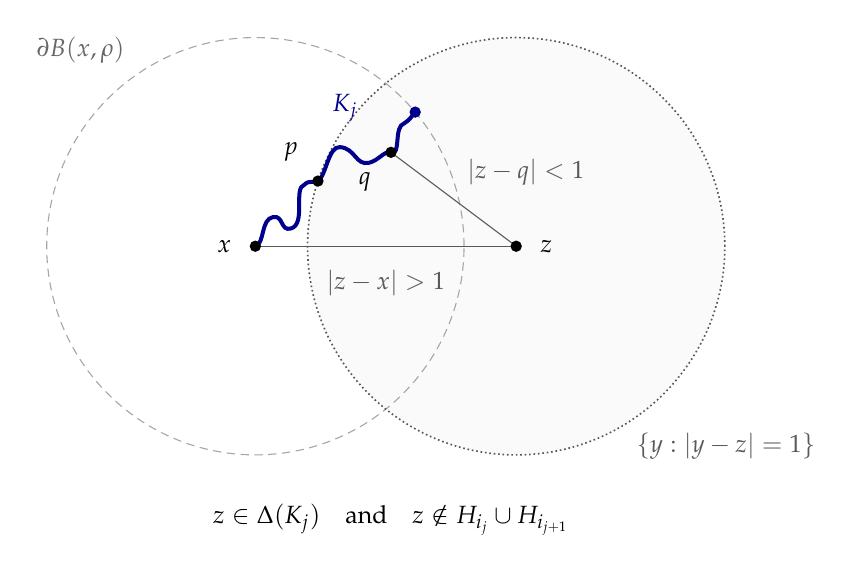
\begin{tikzpicture}[x=2.65cm,y=2.65cm,font=\small,
  point/.style={circle,fill=black,inner sep=1.45pt}]
  \coordinate (X) at (0,0);
  \coordinate (Z) at (1.25,0);
  \coordinate (Q) at (.65,.45);
  \coordinate (P) at (.3,{sqrt(1-.95*.95)});
  \coordinate (F) at ({cos(40)},{sin(40)});

  \fill[black!2] (Z) circle[radius=1];
  \draw[black!35,densely dashed] (X) circle[radius=1];
  \node[black!60,anchor=south east] at (-.58,.83)
    {$\partial B(x,\rho)$};
  \draw[black!65,densely dotted,semithick] (Z) circle[radius=1];
  \node[black!65,anchor=north west] at (1.78,-.85)
    {$\{y:|y-z|=1\}$};

  \draw[black!65] (X) -- node[below=5pt] {$|z-x|>1$} (Z);
  \draw[black!65] (Q) -- node[above right=2pt] {$|z-q|<1$} (Z);

  \draw[blue!55!black,line width=1.45pt,line cap=round]
    (X) .. controls (.045,.01) and (.025,.13) .. (.085,.14)
    .. controls (.135,.15) and (.12,.07) .. (.17,.085)
    .. controls (.245,.105) and (.18,.28) .. (.235,.295)
    .. controls (.26,.32) and (.28,.30) .. (P)
    .. controls (.34,.34) and (.35,.48) .. (.405,.475)
    .. controls (.48,.47) and (.48,.385) .. (.545,.40)
    .. controls (.59,.41) and (.62,.46) .. (Q)
    .. controls (.70,.43) and (.66,.575) .. (.715,.59)
    .. controls (.74,.605) and (.75,.625) .. (F);
  \node[blue!55!black,anchor=south] at (.43,.55) {$K_j$};

  \node[point,label={[label distance=3pt]left:$x$}] at (X) {};
  \node[point,label={[label distance=3pt]right:$z$}] at (Z) {};
  \node[point,label={[label distance=3pt]below left:$q$}] at (Q) {};
  \node[point,label={[label distance=3pt]above left:$p$}] at (P) {};
  \node[point,fill=blue!55!black] at (F) {};
  \node[align=center] at (.65,-1.31)
    {$z\in\Delta(K_j)$\quad and\quad
      $z\notin H_{i_j}\cup H_{i_{j+1}}$};
\end{tikzpicture}

\caption{The strict inequalities $|z-q|<1<|z-x|$, with $x,q\in K_j$,
put $z$ in $\Delta(K_j)$. Connectedness supplies a point $p\in K_j$
with $|z-p|=1$. Both endpoint essential supports are excluded from $\Delta(K_j)$. The shape is schematic: the proof assumes neither an arc nor
a smooth interface nor a tangent at $x$.}
\label{fig:exclusion-continuum}
\end{figure}

\subsection{Disk averages and missing edges}

We begin with continuous probability coordinates.  Their unit-distance
inequality will yield color exclusions from the straddling regions of
the limiting sets.  Small overlaps for missing transition edges will
control the disks removed from the approximation.

For $\epsilon>0$, set
\[
 p_i^\epsilon(q)=\frac1{\pi\epsilon^2}
                     \int_{B(0,\epsilon)}a_i(q+v)\,dv.
\]
These are continuous probability coordinates:
$p_i^\epsilon\ge0$ and $\sum_i p_i^\epsilon=1$ everywhere.
The symmetric-difference estimate for two disks gives
$\operatorname{Lip}(p_i^\epsilon)\le C/\epsilon$, with an absolute
constant $C$.  Approximation by local averages and Lebesgue
differentiation give $p_i^\epsilon\to a_i$ in $L^1_{\rm loc}$ and
almost everywhere as $\epsilon\downarrow0$.

\begin{lemma}[Disk inequalities and support detection]
\label{lem:transitions-disk-averages}
For every pair $q,z\in\R^2$ with $|q-z|=1$ and every label $i$,
\begin{equation}
 p_i^\epsilon(q)+p_i^\epsilon(z)\le1.
 \label{eq:source-17}
\end{equation}
If $q_n\to q$, $\epsilon_n\to0$, and
$\liminf_n p_i^{\epsilon_n}(q_n)>0$, then $q\in H_i$.
\end{lemma}

\begin{proof}
Translate $q$ and $z$ by the same vector uniformly distributed in
$B(0,\epsilon)$.  Almost every such translation puts both points in
the typical set.  They cannot then both have color $i$; averaging
proves \eqref{eq:source-17}.  Thus this inequality has no exceptional
unit pairs.  For the last assertion, every neighborhood of $q$
eventually contains $B(q_n,\epsilon_n)$, and the stated lower bound
makes its intersection with $A_i$ have positive area.
\end{proof}

\begin{lemma}[A missing edge has small overlap]
\label{lem:transitions-missing-edge}
If $ij\notin\Gamma_x$, there is a ball $B$ about $x$ such that, for
every smaller ball $B'$ with $\overline{B'}\subset B$,
\begin{equation}
 \int_{B'}p_i^\epsilon(q)p_j^\epsilon(q)\,dq=o(\epsilon).
 \label{eq:source-18}
\end{equation}
For any ball $B''$ with $\overline{B''}\subset B'$ and any fixed
$\alpha>0$, the set
\[
 \{q\in B'':p_i^\epsilon(q)>\alpha,\quad
                    p_j^\epsilon(q)>\alpha\}
\]
can be covered by finitely many open disks whose total radii tend to
zero as $\epsilon\downarrow0$.  Every point of the set lies in a disk
interior.
\end{lemma}

\begin{proof}
The negation of \eqref{eq:source-14}, and nonnegativity of $D_{ij}$,
give a ball $B$ with $D_{ij}(B,h)=o(|h|)$.  More explicitly, for all
sufficiently small $r>0$ put
\[
 \omega(r)=\sup_{0<|h|\le r}\frac{D_{ij}(B,h)}{|h|};
 \qquad \omega(r)\longrightarrow0.
\]
For independent uniform vectors $h_1,h_2\in B(0,\epsilon)$, expand the
product of the two disk averages and integrate over $q\in B'$.  When
$\epsilon<\dist(\overline{B'},\R^2\setminus B)$, the change of root
$r=q+h_1$ bounds the area where $c(q+h_1)=i$ and $c(q+h_2)=j$ by
\[
 D_{ij}(B,h_2-h_1)\le 2\epsilon\omega(2\epsilon).
\]
For $h_1=h_2$ the simultaneous event is empty.  Fubini now gives
\eqref{eq:source-18}, with a bound uniform over the two shifts.

Take a square grid with side $\ell=c_\alpha\epsilon$, where
$c_\alpha>0$ is fixed small enough that the Lipschitz oscillation of
either probability on a square is at most $\alpha/2$.  Select all
squares touching the displayed violation set in $B''$.  Their number
$N_\epsilon$ is finite, and for small $\epsilon$ each lies in $B'$ and
has both probabilities at least $\alpha/2$ throughout.  Disjointness
of their interiors and \eqref{eq:source-18} imply
\[
 N_\epsilon\ell^2\frac{\alpha^2}{4}=o(\epsilon),
 \qquad N_\epsilon\epsilon=o(1).
\]
Cover every selected closed square by the open disk with the same
center and radius $\ell$.  These disks strictly contain the squares
and have total radii $N_\epsilon\ell=o(1)$.
\end{proof}

\subsection{Graph-valued maps outside small core disks}

The preceding overlap bound allows us to remove all simultaneous
threshold violations associated with missing edges.  Fix
$0<\alpha<1/5$, and define
\begin{equation}
 q_i^\epsilon(z)=
 \frac{(p_i^\epsilon(z)-\alpha)_+}
      {\sum_{k\in\mathcal I}(p_k^\epsilon(z)-\alpha)_+},
 \qquad i\in\mathcal I.
 \label{eq:source-22}
\end{equation}
The denominator is positive because the five probabilities sum to one.
Thus $q^\epsilon$ is a continuous map into the simplex of probability
vectors on $\mathcal I$.  Let $\mathscr G$ be the one-skeleton of that
simplex, realized as the complete graph on its five vertices.  In
particular, $q_i^\epsilon(z)>0$ if and only if
$p_i^\epsilon(z)>\alpha$.

Choose a closed square $Q$ of side ten with
$\partial Q\cap\mathcal L=\varnothing$.  Such a square is obtained by
a small translation: local finiteness leaves only finitely many points
to avoid near the boundary of all squares in that translation family.
Choose a larger closed square $Q'$ containing $Q$ in its interior, and
write $L_0=\mathcal L\cap Q'$, a finite set by
Theorem~\ref{thm:cyclic-local-finiteness}.

\begin{lemma}[Small holes and tree fillings]
\label{lem:interfaces-hole-maps}
There are $\epsilon_n\downarrow0$ and finite families $\mathcal H_n$
of open disks with pairwise disjoint closures such that their total
radii tend to zero and the following hold for all sufficiently large
$n$.
\begin{enumerate}
\item For each $x\in L_0$, precisely one disk of $\mathcal H_n$ is
designated the core disk $B_{n,x}$ and contains $x$ in its interior.
Different points give different core disks.  If $x\in Q$, then
$\overline{B_{n,x}}\subset\operatorname{int}(Q)$; if $x\notin Q$, then
$\overline{B_{n,x}}\cap Q=\varnothing$.
\item The map $q^{\epsilon_n}$ takes values in $\mathscr G$ on
$Q\setminus\bigcup_{B\in\mathcal H_n}B$.
\item There is a continuous map
\begin{equation}
 g_n:Q\setminus\bigcup_{x\in L_0\cap Q}B_{n,x}
       \longrightarrow\mathscr G
 \label{eq:source-23}
\end{equation}
equal to $q^{\epsilon_n}$ outside all the open disks of
$\mathcal H_n$.  It is obtained by filling the non-core disks through
trees, preserving their boundary values.
\end{enumerate}
\end{lemma}

\begin{proof}
Fix a small $\delta>0$.  Start with the original core disks
$B(x,\delta)$, $x\in L_0$, and put
\[
 M_\delta=Q'\setminus\bigcup_{x\in L_0}B(x,\delta).
\]
This is compact, and every $\Gamma_z$, $z\in M_\delta$, is a forest,
including any isolated vertices.  For each nonedge of $\Gamma_z$,
Lemma~\ref{lem:transitions-missing-edge} supplies a ball on which the
corresponding simultaneous threshold violations admit finite open
disk covers with total radii tending to zero as $\epsilon\to0$.
There are finitely many nonedges, so choose one radius $s_z>0$
working for all of them.  More explicitly, choose it small enough
to have the transition estimate on $B(z,3s_z)$, the integral
estimate on $B(z,2s_z)$, and the disk covers for violations in
$B(z,s_z)$.  The covers include the violation points in the
interiors of their disks.

Choose finitely many balls $B(z,s_z)$ covering $M_\delta$, and let
$\lambda_\delta>0$ be a Lebesgue number of this cover on $M_\delta$.
For each selected ball, mark all the disks covering violations for
its forest's nonedges.  These additional disks form a finite family
whose total radii $m_{\delta,\epsilon}$ tend to zero for this fixed
$\delta$.  At a point of $M_\delta$ outside all marked disks, the
positive coordinates of \eqref{eq:source-22} form a clique in the
forest of every selected ball containing the point.  They therefore
number at most two, and a two-element set is a forest edge.  This
proves the required local graph-valued assertion.

We next merge disks until their closures are pairwise disjoint.
Whenever two current disks have intersecting closures, replace them
by an open disk strictly containing both closures, with radius at
most the sum of their radii plus a prescribed positive error.
An enclosing disk with radius at most the sum exists by choosing its
center on the line of centers; in the containment case the larger
disk suffices.  A slight enlargement makes containment strict.
Each merge reduces the finite number of disks, so the sum of all
enlargement errors can be made less than any specified
$\eta>0$, using the initial number as a bound on the number of merges.

A final disk is called core if its merger class contains an original
core disk.  Every final boundary avoids every original disk interior.
The total final radii are at most
\[
 |L_0|\delta+m_{\delta,\epsilon}+\eta,
\]
and each final non-core radius is at most
$m_{\delta,\epsilon}+\eta$.  Take $\delta_n\downarrow0$.
After fixing $\delta_n$, its finite cover, and its Lebesgue number,
choose $\epsilon_n$ and the merger errors so that
\[
 \epsilon_n<\min\{1/n,\epsilon_{n-1}/2\},\qquad
 m_{\delta_n,\epsilon_n}+\eta_n
   <\min\{1/n,\lambda_{\delta_n}/3\},
\]
omitting the preceding-$\epsilon$ condition at $n=1$.
The total final radii now tend to zero.

For large $n$, no final disk can contain two distinct points of $L_0$:
its diameter is smaller than their minimum positive separation.
Every original core disk belongs to some final disk, so this gives
exactly one core disk for each point.  Since a disk of radius $r$
containing $x$ lies in $B(x,2r)$, the positive distances between the
finitely many points of $L_0$ and $\partial Q$ give the asserted
positions of the core disks.

Consider a final non-core disk whose closure meets $Q$.  Its vanishing
diameter puts its entire closed disk inside $Q'$ for large $n$.
Moreover, its closure is disjoint from every final core closure,
and these final core disks contain all the original core disks.
It therefore lies outside all original core interiors, hence in
$M_{\delta_n}$.  Its diameter is less than $\lambda_{\delta_n}$,
so its entire closed disk lies in one selected forest ball.
Its boundary avoids all original marked interiors.  The original
map $q^{\epsilon_n}$ thus maps that boundary into the selected
forest, and its connected boundary image lies in one component
tree, possibly a single vertex.  A finite tree is contractible,
so the boundary map extends continuously over the closed disk
with values in that tree.  If the disk crosses $\partial Q$,
make the extension on the whole disk and restrict it to $Q$.

Outside all final open disks, every point of $Q$ belongs to
$M_{\delta_n}$ and avoids all original marked disks, so the original
map is graph-valued there.  Paste it to the finitely many tree
extensions.  Their closed disks have disjoint closures and agree
with the original map on their boundaries, so finite pasting proves
\eqref{eq:source-23}.  Empty disk lists require no operation.
\end{proof}

\subsection{A nontrivial core boundary}

We will repeatedly use the following area estimate.  For a closed
disk $\overline{B(u,r)}$ with $r<1$, every point at distance one from
some point of that disk belongs to
\[
 E(u,r)=\{z:1-r\le |z-u|\le1+r\}.
\]
The triangle inequality proves this containment, and the annulus
has area $4\pi r$.  For the families in
Lemma~\ref{lem:interfaces-hole-maps}, write
\begin{equation}
 E_n=\bigcup_{B(u,r)\in\mathcal H_n}E(u,r),
 \qquad
 |E_n|\le4\pi\sum_{B(u,r)\in\mathcal H_n}r\longrightarrow0.
 \label{eq:interfaces-annulus-area}
\end{equation}
Here all radii are less than one for large $n$.  If $z\notin E_n$,
no exact unit-distance point from $z$ lies in any closed hole disk,
regardless of how many disks there are.

\begin{lemma}[A cover obstruction on a square]
\label{lem:interfaces-cover}
A closed square of side ten has no relatively open cover of
multiplicity at most two and mesh at most two, where mesh is the
supremum of the Euclidean diameters of its members.
\end{lemma}

\begin{proof}
Compactness gives a finite subcover $U_1,\ldots,U_N$ with the same
bounds.  Choose $z_a\in U_a$.  There is a continuous partition of
unity $\phi_a$ with $\phi_a(z)>0$ only when $z\in U_a$; explicitly,
use $\dist(z,Q\setminus U_a)$ and normalize their sum.  None of the
$U_a$ equals $Q$, since its diameter would exceed two, so these
distance functions are well defined.  Set
\[
 F(z)=\sum_{a=1}^N\phi_a(z)z_a.
\]
Convexity gives $F(Q)\subset Q$.  At most two weights are positive
at any point, so the image is contained in the finite union of
segments $[z_a,z_b]$ and singleton vertices.  Also
\[
 |F(z)-z|
 \le\sum_a\phi_a(z)|z_a-z|\le2.
\]
For any $y\in Q$ with $\dist(y,\partial Q)>2$, the continuous map
$z\mapsto y+z-F(z)$ takes $Q$ into $Q$, since its image lies in
the closed radius-two disk about $y$.  The Brouwer fixed point
theorem, in its planar form
\citep[Theorem~1.9]{Hatcher2002}, therefore supplies a fixed point,
and at that point $F(z)=y$.  Thus $F(Q)$ contains the nonempty open
central region $\{y\in Q:\dist(y,\partial Q)>2\}$, impossible for a
finite union of segments.
\end{proof}

\begin{lemma}[Non-null core loops]
\label{lem:interfaces-core-loop}
For all sufficiently large $n$, some core disk $B_{n,x}$ contained
in $Q$ has a boundary loop whose image under $g_n$ is not null
homotopic in $\mathscr G$.
\end{lemma}

\begin{proof}
Otherwise, along an infinite subsequence all the core boundary
loops are null homotopic.  Extend each such loop over its disk
in $\mathscr G$, and paste to obtain a continuous map
$\widetilde g_n:Q\to\mathscr G$, still equal to $q^{\epsilon_n}$
outside all holes.  For each $i\in\mathcal I$, take the components
of the relatively open set
\[
 U_{n,i}=\{z\in Q:(\widetilde g_n(z))_i>0\}.
\]
The square and its relatively open subsets are locally path
connected; hence these components are open and path connected.
They form a cover of $Q$ of multiplicity at most two, since every
point of $\mathscr G$ has at most two positive coordinates.

We claim that the mesh of this component cover is at most $1+o(1)$.
If not, after restricting to a subsequence there are a fixed
constant $c>0$, a fixed label $i$, and paths in $U_{n,i}$ joining
points at distance greater than $1+c$.  Replace either endpoint
lying in a hole by a boundary point on the path.  The path must
exit that disk because the other endpoint is distant, and the
replacement changes the endpoint by at most the disk's diameter.
If both endpoints require replacement, their disks are distinct
for large $n$.  On every hole boundary the original map is
preserved.  Thus the replacement endpoints $a_n,b_n$ satisfy
\[
 p_i^{\epsilon_n}(a_n)>\alpha,\qquad
 p_i^{\epsilon_n}(b_n)>\alpha
\]
and remain at distance at least $1+c-o(1)$.  Pass to limits
$a_n\to a$, $b_n\to b$ in $Q$, with $|a-b|>1$.
Lemma~\ref{lem:transitions-disk-averages} gives $a\in H_i$.

Choose a sufficiently small fixed open plane ball $U$ about $a$.
For all large $n$ and every $z\in U$, the distances to $a_n$ and
$b_n$ are strictly below and strictly above one, respectively.
Continuity along the path supplies a point at exact distance one
from $z$.  If $z\notin E_n$, every such crossing point is outside
all closed hole disks by \eqref{eq:interfaces-annulus-area}.
At this point $\widetilde g_n=q^{\epsilon_n}$ and its $i$th
coordinate is positive, so $p_i^{\epsilon_n}>\alpha$.
The pointwise inequality \eqref{eq:source-17} therefore gives
$p_i^{\epsilon_n}(z)\le1-\alpha$.

It follows that
\begin{equation}
 \alpha |A_i\cap U|
 \le
 \norm{p_i^{\epsilon_n}-a_i}_{L^1(U)}
      +\alpha|E_n\cap U|
 \longrightarrow0.
 \label{eq:interfaces-mesh-measure}
\end{equation}
The convergence uses local $L^1$ convergence of disk averages and
\eqref{eq:interfaces-annulus-area}.  This contradicts $a\in H_i$,
which requires positive $A_i$-measure in $U$.  The mesh claim
follows.  For large $n$ the mesh is therefore at most two,
contradicting Lemma~\ref{lem:interfaces-cover}.  This argument also
rules out the possibility of having no core disks in $Q$.
\end{proof}

\subsection{Graph words and annular crossings}

We now have a graph-valued map with a non-null loop around a core disk.
To turn that loop into connected crossing sets, we identify edge
midpoints that every homotopic loop must meet.  We first recall the
reduced-path argument for graphs; compare
\citet[Section~1.A]{Hatcher2002}.

\begin{lemma}[Midpoint detection by a reduced circuit]
\label{lem:interfaces-graph-word}
Let $G$ be a finite connected simple graph.  Every nontrivial free
homotopy class of loops in $G$ has a nonempty cyclically reduced closed
edge word $W$.  Such a word contains a simple cycle.  Moreover, if $m$
is the midpoint of any edge occurring in $W$, every loop freely
homotopic to a nonzero power of $W$ meets $m$.
\end{lemma}

\begin{proof}
An edge path is reduced when consecutive edges never reverse each
other, and a reduced closed edge path is cyclically reduced when its
last and first edges do not reverse each other either.  Paths between
vertices, up to homotopy fixing their endpoints, have unique reduced
edge representatives.  One way to see this is to construct the covering
tree based at a vertex $v$: its vertices are reduced paths starting at
$v$, and its edges append one edge and then reduce.  Deleting the last
edge gives the unique path toward the empty word, so this covering
graph is a tree.  The map recording the endpoint is a bijection on
each incident-edge star and hence a covering map.  Lifting a path to
this tree and contracting it to the unique simple path between its
lifted endpoints proves existence and uniqueness of the reduced
representative.  These contractions apply to arbitrary continuous
paths: their compact images in the locally finite covering tree lie
in finite subtrees.

Move a loop's basepoint to a vertex along a path, reduce its edge
word, and successively trim inverse first and last edges.  The result
is cyclically reduced and is empty precisely when the loop is null
homotopic.  Moving the basepoint, or following the basepoint during a
free homotopy, changes the based class by conjugation.

We record how conjugation affects a nonempty cyclically reduced word.
First reduce the conjugating path $P$ in $PWP^{-1}$.  At the last edge
of $P$, cancellation against one end of $W$ shortens $P$ and moves
one edge of $W$ to its other end.  This only rotates $W$ cyclically.
Cancellation at both ends of $W$ at once is impossible because $W$
is cyclically reduced.  If there is no cancellation at either end,
the conjugating path is simply removed when the whole closed word is
cyclically trimmed.  Induction on the length of $P$ shows that
conjugation leaves the cyclically reduced circuit unchanged up to
cyclic rotation.

A nonzero power of $W$ is already cyclically reduced: concatenate
copies of $W$ for a positive power, or copies of its reversed inverse
for a negative power.  Its cyclic reduction therefore uses every edge
of $W$.  On the other hand, $G\setminus\{m\}$ deformation retracts onto
the graph with the edge containing $m$ deleted: contract its two
remaining half-open stubs to their endpoint vertices.  A loop avoiding
$m$ consequently has a reduced circuit using no such edge, and cannot
be freely homotopic to a nonzero power of $W$.

Finally, take a shortest nonempty subloop between repeated vertices
of $W$.  It has no repeated interior vertex.  Its length is not one,
since $G$ has no loop edges, and is not two, since that would be an
immediate reversal in a simple graph.  Thus it is a simple cycle.
\end{proof}

\begin{lemma}[A connected midpoint preimage crosses the annulus]
\label{lem:interfaces-annular-crossing}
Let $B$ be an open disk containing $x$, with
$\overline B\subset B(x,\rho)$, and set
$\mathcal A=\overline{B(x,\rho)}\setminus B$.
Suppose $g:\mathcal A\to G$ is continuous, where $G$ is a finite
connected simple graph, and the image of the counterclockwise inner
boundary has nonempty cyclically reduced word $W$.  If $m$ is the
midpoint of an edge occurring in $W$, then $g^{-1}(\{m\})$ has a
compact connected component meeting both boundary circles of
$\mathcal A$.
\end{lemma}

\begin{proof}
Every ray from $x$ meets $\partial B$ once, at a positive radius
$r(\theta)$ depending continuously on the angle.  Radial interpolation
between $r(\theta)$ and $\rho$ identifies $\mathcal A$ with a closed
annulus.  In particular, winding number about $x$ identifies its
fundamental group with $\Z$, with the counterclockwise inner boundary
as generator.

Put $Z=g^{-1}(\{m\})$.  This is a compact metric space.  Suppose no
component of $Z$ meets both boundaries, and write
$I=Z\cap\partial B$ and $O=Z\cap\partial B(x,\rho)$ for its compact
inner and outer contact sets.  We first obtain a disjoint compact partition
$Z=Z_1\sqcup Z_2$ with $I\subset Z_1$ and $O\subset Z_2$.

In any compact metric space, a point's component is the intersection
of all of its clopen neighborhoods.  Indeed, this intersection
contains the component.  If it were disconnected, its two nonempty
compact parts could be enclosed in disjoint open sets.  A finite
intersection of clopen neighborhoods already lies in their union,
by compactness of the complement of that union.  Intersecting this
clopen set with the open set containing the original point gives
a smaller clopen neighborhood omitting the other part, a
contradiction.  The intersection is therefore connected and equals
the component.

Thus, for each point of $I$ and each point of $O$, some clopen
neighborhood of the first omits the second.  Compactness of $O$
permits a finite intersection producing a clopen neighborhood of
the first point disjoint from all of $O$.  Compactness of $I$
then permits a finite union containing all of $I$ and still
disjoint from $O$.  Take this union as $Z_1$ and its complement in
$Z$ as $Z_2$.  If either $I$ or $O$ is empty, use $Z_1=\varnothing$
or $Z_1=Z$, respectively.  This proves the partition assertion.

The set
\[
 C_1=Z_1\cup\overline B
\]
is compact, lies in the open outer disk, and is disjoint from $Z_2$.
Choose a sufficiently fine translated square grid, with $x$ on no
grid line, and take every closed grid cell meeting $C_1$.  Their
finite union $V$ lies in the open outer disk and avoids $Z_2$, by the
positive compact separations.  Also $C_1\subset\operatorname{int}(V)$:
at a point of $C_1$ on a grid edge or vertex, all adjacent cells
are included.  Consequently $\partial V$ lies in $\mathcal A$
and avoids $Z_1\cup Z_2=Z$.

Orient each selected square boundary counterclockwise and cancel
shared edges.  The remaining edges lie on $\partial V$ and form
a balanced finite directed chain, so they decompose into closed
polygonal loops.  Their total winding about $x$ is one.  Indeed,
winding is additive before and after cancellation, and exactly one
selected square contains $x$ in its interior; its winding is one
and that of every other selected square is zero.  At least one
of the resulting loops has nonzero winding, say $d$.  Its image
under $g$ avoids $m$, but the annulus calculation makes that image
freely homotopic to $W^d$.  This contradicts
Lemma~\ref{lem:interfaces-graph-word}.
\end{proof}

\subsection{Limiting continua and simultaneous color exclusions}

\begin{proof}[Proof of Proposition~\ref{prop:interface-cycle}]
Use the maps of Lemma~\ref{lem:interfaces-hole-maps} and the
non-null loops from Lemma~\ref{lem:interfaces-core-loop}.
Since $L_0\cap Q$ is finite, pass to a subsequence with a fixed
$x\in L_0\cap\operatorname{int}(Q)$ whose core boundary loop
is non-null at every index.  Choose $\rho>0$ so small that
$\overline{B(x,\rho)}\subset\operatorname{int}(Q)$ and contains no
other point of $L_0$.  Decreasing $\rho$ if necessary, the other
core closed disks are disjoint from $\overline{B(x,\rho)}$ for
large $n$, while
$\overline{B_{n,x}}\subset B(x,\rho)$.  The map $g_n$ is therefore
defined on the closed annulus
\[
 \mathcal A_n=\overline{B(x,\rho)}\setminus B_{n,x}.
\]
The inner disk contains $x$ strictly; its possibly eccentric
position causes no difficulty for the radial annulus coordinates
used in Lemma~\ref{lem:interfaces-annular-crossing}.

Let $W_n$ be a nonempty cyclically reduced circuit representing the
image of the counterclockwise inner boundary.  By
Lemma~\ref{lem:interfaces-graph-word}, it contains a simple cycle.
There are only finitely many simple cycles in the complete graph
on five vertices.  Pass to a subsequence with one chosen cycle,
of length $\ell\in\{3,4,5\}$, and label its vertices
$i_0,\ldots,i_{\ell-1}$ in cyclic order.  For each of its edge
midpoints $m_j$, Lemma~\ref{lem:interfaces-annular-crossing} gives
a compact connected component
\[
 K_{n,j}\subset g_n^{-1}(\{m_j\})\cap\mathcal A_n
\]
meeting both annulus boundaries.

Take Hausdorff limits along a common further subsequence for the
finitely many indices $j$:
\[
 K_{n,j}\longrightarrow K_j\subset\overline{B(x,\rho)}.
\]
The nonempty compact subsets of a compact metric space are compact
in the Hausdorff metric.  For completeness, finite nets give total
boundedness of this hyperspace, and for a Hausdorff-Cauchy sequence
the set of limits of convergent point selections is its nonempty
compact Hausdorff limit, proving completeness.  Connectedness also
passes to the limit: a disconnection of $K_j$ into two nonempty
compact parts gives disjoint separated neighborhoods containing
every sufficiently close $K_{n,j}$, with each neighborhood met,
contradicting connectedness of $K_{n,j}$.

Each $K_{n,j}$ meets $\partial B_{n,x}$.  These contact points tend
to $x$, because the disk contains $x$ and its diameter tends to
zero.  Hence $x\in K_j$.  Outer-boundary contact and compactness
likewise give $K_j\cap\partial B(x,\rho)\ne\varnothing$.
In particular each $K_j$ is nontrivial.

We prove the support exclusion for either endpoint
$i\in\{i_j,i_{j+1}\}$.  At a point of $K_{n,j}$ outside all holes,
$g_n=q^{\epsilon_n}$ has value $m_j$, whose two endpoint
coordinates are $1/2$.  Formula~\eqref{eq:source-22} therefore gives
$p_i^{\epsilon_n}>\alpha$ there.

Fix any closed ball $U$ of positive radius contained in
$\Delta(K_j)$.  The strict inequalities defining the straddling
region hold with a positive uniform margin on $U$.  For every
$z$, either distance extremum changes by at most
$d_{\rm H}(K_{n,j},K_j)$ when $K_j$ is replaced by $K_{n,j}$.
Thus, for all sufficiently large $n$, the distances from every
$z\in U$ to points of $K_{n,j}$ straddle one.  The continuous
image of the connected set $K_{n,j}$ under $q\mapsto|z-q|$
is an interval, so some point of $K_{n,j}$ is at exact distance
one from $z$.

For $z\in U\setminus E_n$, that point is outside every closed hole
disk.  The preceding endpoint probability bound and
\eqref{eq:source-17} give $p_i^{\epsilon_n}(z)\le1-\alpha$.
Exactly as in \eqref{eq:interfaces-mesh-measure},
\[
 \alpha |A_i\cap U|
 \le \norm{p_i^{\epsilon_n}-a_i}_{L^1(U)}
       +\alpha |E_n\cap U|\longrightarrow0.
\]
Thus $A_i$ has zero measure in $U$.  Every point of the open set
$\Delta(K_j)$ lies in the interior of such a ball, and consequently
has a neighborhood of zero $A_i$-measure.  By the definition of
$H_i$, this proves $H_i\cap\Delta(K_j)=\varnothing$ for both
endpoint labels.

Finally, connectedness and the two contact conditions imply
\[
 \{|q-x|:q\in K_j\}=[0,\rho].
\]
Choose points in $K_j$ at radii $\rho/k$, $k\ge2$, and pass to a
subsequence of their unit directions converging to some $v_j\in S$.
Relabel these points as $q_{j,k}$.  They supply the required
sequences and complete the proof.
\end{proof}

\section{Angular obstructions and the final contradiction}
\label{sec:angular}

We now show that none of the three cycle lengths supplied by
Proposition~\ref{prop:interface-cycle} is possible.  Fix its common
center \(x\), cyclically index the cycle labels by \(j\), and let
edge \(j\) join labels \(j\) and \(j+1\).  Write \(K_j\) for its
continuum and \(v_j\) for its limiting unit direction.  Thus there
are points
\[
 q_{j,n}=x+r_{j,n}w_{j,n}\in K_j,\qquad
 r_{j,n}>0,\quad r_{j,n}\longrightarrow0,\quad
 w_{j,n}\in S,\quad w_{j,n}\longrightarrow v_j.
\]
The rays used below record only these selected limiting directions
\(v_j\); no straight ray segment is assumed to lie in \(K_j\).
All palettes in this section are at this fixed center.  As before,
\(R\) rotates by \(\kappa=\pi/3\), and \(J\) by \(\pi/2\).

\subsection{Restrictions on the two sides of the unit circle}

The one-sided strips below are a counterpart of the complementary-color
strips in \citet[Proposition~9]{SokolovVoronov2025}. Related circle and
complementary-arc arguments also occur in
\citet[Sections~3--5]{Voronov2025Interval}, for a positive interval of
forbidden distances. We use only the single forbidden distance one;
the input is the exclusion continua just extracted.

Let \(\mathcal B\subset S\) be the finite, antipodally symmetric
set of directions perpendicular to at least one \(v_j\).
At \(e\notin\mathcal B\), give edge \(j\) sign \(+\) or \(-\)
according as \(e\cdot v_j\) is positive or negative.  Let \(O(e)\)
be the set of labels remaining after the endpoints of every positive
edge are removed, and let \(I(e)\) be the set remaining after the
endpoints of every negative edge are removed.  Labels outside the
cycle belong to both sets.

\begin{lemma}[One-sided strip restrictions]\label{lem:angular-strips}
Both \(O(e)\) and \(I(e)\) are nonempty for every
\(e\notin\mathcal B\).  On an angular neighborhood of \(e\), an
open strip just outside radius one uses only \(O(e)\), and an open
strip just inside radius one uses only \(I(e)\), in both cases up
to plane-null sets.  Moreover,
\begin{equation}\label{eq:source-25}
 P_x(e)\cap O(e)\ne\varnothing,
 \qquad P_x(e)\cap I(e)\ne\varnothing
 \quad\text{for almost every }e\in S\setminus\mathcal B.
\end{equation}
\end{lemma}

\begin{proof}
For a positive edge sign, the identity
\[
 \abs{x+e-q_{j,n}}^2
 =1+r_{j,n}^2-2r_{j,n}(e\cdot w_{j,n})
\]
is strictly less than one for some sufficiently large fixed \(n\).
By continuity, the strict inequality holds when \(e\) varies in
a small angular neighborhood and its radius increases slightly
above one.  Such points have distance greater than one from
\(x\in K_j\) and less than one from \(q_{j,n}\in K_j\); they lie
in \(\Delta(K_j)\).  Proposition~\ref{prop:interface-cycle} excludes both
endpoint essential supports there.  If the sign is negative,
the displayed distance is greater than one for large \(n\), and
the same argument at radii slightly below one gives the inner
strip.  There are finitely many edges, so the angular neighborhoods
and positive radial widths can be intersected.  An empty allowed
set would exclude every color from a nonempty open strip, contrary
to the measurable partition.

Cover \(S\setminus\mathcal B\) by countably many smaller arcs
on each of which all signs are constant and both strip restrictions
hold with positive widths.  For each such arc, polar-coordinate
Fubini gives the relevant restriction almost everywhere angularly
for almost every radius in its permitted interval.  Impose no
condition from that arc outside its permitted interval; its failures
then exclude only a null set from the whole radial half-line.
Intersect these countably many full-measure radial conditions with the
full-measure condition of typical sampling at center \(x\).
Choose radii from this intersection tending to one from above.
For each fixed arc the outer restriction eventually holds along
the entire sequence.  A weak-* subsequential trace in
\(\mathcal W_x\) has zero coordinates for the excluded labels
on that arc.  Its coordinates sum to one, and its positive
coordinates belong to \(P_x\) almost everywhere, so it supplies
an outer allowed palette member.  Countably many arcs suffice.
A separate sequence tending to one from below proves the inner
assertion.  The two sides need not use the same trace.
\end{proof}

\subsection{Exclusion of a five-cycle}

\begin{proposition}\label{prop:angular-five}
The extracted interface cycle cannot have length five.
\end{proposition}

\begin{proof}
Index its five labels modulo five.  A label belongs to \(I(e)\)
exactly when its two incident signs are positive, and to \(O(e)\)
exactly when both are negative.  Their nonemptiness requires a
pair of consecutive signs of each kind.  If there were two or
more runs of each kind, the two required runs of length at least
two and the other two nonempty runs would occupy at least six
positions.  Thus the five signs consist of one positive run and
one negative run, of lengths two and three in some order.

The allowed sets are the internal vertices of these runs, of
sizes one and two.  They are disjoint.  The palette size bound
\eqref{eq:source-13} and \eqref{eq:source-25} imply that almost
every palette is a pair, containing one vertex from each allowed
set.  Put \(D_i=\{i,i+2\}\).  After a cyclic relabeling, the
length-two run occupies edges \(0,1\), with middle vertex \(1\),
and the length-three run occupies edges \(2,3,4\), with internal
vertices \(3,4\).  The two possible palettes are therefore
\(D_1=\{1,3\}\) and \(D_4=\{4,1\}\), whose indices differ by
two modulo five.  Reversing every sign interchanges the two
allowed sets and preserves these options.  Consequently the
palette options at antipodal directions are identical.

Choose a direction on a full six-position \(R\)-orbit for which
all the preceding almost-everywhere assertions and
\eqref{eq:source-12} hold.  Write \(p_j\in\Z/5\Z\) for the
index of its palette \(D_{p_j}\) at \(R^je\).  Two diagonals
\(D_a,D_b\) are disjoint exactly when \(b-a=\pm1\) modulo five.
Thus successive indices make steps \(\varepsilon_j\in\{1,-1\}\),
including the closing step from position five to position zero.
For antipodal positions \(j,j+3\), the common two-element option
set allows index difference only \(0\) or \(\pm2\).
But the possible sums of three steps are \(-3,-1,1,3\); none
is zero modulo five, and a sum is \(\pm2\) modulo five only if
all three steps have the same sign.  Every consecutive triple
of steps must therefore be constant.  Overlapping triples force
all six signs to agree, whereas six equal steps do not close
modulo five.  This is the desired contradiction.
\end{proof}

\subsection{Four-cycle words and projective ray geometry}

Suppose next that the cycle labels are \(0,1,2,3\), with outsider
\(X\), and put \(U=\{0,2\}\), \(V=\{1,3\}\).
If \(X\notin P_x(e)\), the two requirements in
\eqref{eq:source-25} force a consecutive pair of positive signs
and a consecutive pair of negative signs.  Hence the four signs
are a cyclic run of two of each sign, which we call a
\emph{split}.  The two allowed sets, after removing \(X\), are
the opposite middle vertices of the runs.  They determine a
diagonal \(d(e)\in\{U,V\}\), and \(d(-e)=d(e)\).

Define the effective state \(p(e)\) to be \(X\) whenever
\(X\in P_x(e)\), and otherwise to be the forced diagonal
\(d(e)\).  The group represented by this state is contained
in the palette: it is the singleton \(\{X\}\) in the first
case and the entire diagonal in the second.  Consequently,
\begin{equation}\label{eq:source-26}
 p(e)\ne p(Re),\qquad
 p(e)=p(-e)\ \text{if both states are different from }X,
 \quad\text{almost everywhere}.
\end{equation}
If a diagonal occurs only on a null set, the remaining
singleton-versus-pair state system contradicts
Lemma~\ref{lem:transitions-two-state}; a single remaining state
already contradicts the first assertion in \eqref{eq:source-26}.
We may therefore suppose that both diagonal states have positive
angular measure.

For a nonparallel pair of density-one directions of the \(U\)
and \(V\) state sets, the density conclusion of
Lemma~\ref{lem:palette-transfer} excludes all four cycle labels
at their sum with \(x\).  That sum has density one of \(X\).
Lemma~\ref{lem:transitions-strict-separation} now applies to these
three represented groups.  If \(F_U,F_V\) denote the compact
angular essential supports of the diagonal state sets, then
\[
 F_D\cap RF_D=\varnothing\qquad(D=U,V).
\]
The same holds for \(R^{-1}\).  Compactness provides a common
positive angular separation margin.

Choose a dense conull set \(G\) of angular parameters, invariant
under addition of \(\kappa\), on which all six orbit positions
avoid \(\mathcal B\), satisfy the state rules, and belong to
\(F_U\) or \(F_V\) whenever the respective state occurs.  Define
\[
 w(t)_j=p(e^{i(t+j\kappa)}),\qquad j\in\Z/6\Z,
 \quad t\in G.
\]
There exists \(\eta>0\) such that whenever \(t,t'\in G\)
have circular angular distance less than \(\eta\), a diagonal
at any position of \(w(t)\) cannot equal a diagonal at an
adjacent position of \(w(t')\).  Indeed, such equality would
give points of the same compact essential support at angular
distance less than the margin from an \(R\)- or \(R^{-1}\)-pair.
We refer to this as the cross-word restriction.

\begin{lemma}[Six-position word alternatives]\label{lem:angular-words}
Every word \(w(t)\) contains \(X\), and all its \(X\) positions
have the same parity.  Every direction outside \(\mathcal B\)
is split.
\end{lemma}

\begin{proof}
A word without \(X\) alternates \(U,V\) by adjacent inequality,
contradicting the antipodal equality in \eqref{eq:source-26}.
Suppose that \(X\) occurs on both parities.  Any pair of its
opposite-parity positions must be antipodal, since otherwise
they are adjacent on the six-cycle.  There are exactly two
such occurrences: fixing one on each parity prevents any
additional occurrence on either parity.  Cyclically shift
them to positions zero and three.  Positions one and two
are distinct non-\(X\) states, and their antipodes four and
five have the same respective values.  Thus the word is a
three-periodic permutation of \(X,U,V\).

Such a word is isolated under the cross-word restriction.
In any compatible nearby word, each of its positions zero
and three has neighbors \(U,V\) in the original word; it
must therefore be \(X\).  The remaining four positions are
non-\(X\) by their own adjacent inequality.  If the original
positions one and two are \(U,V\), the cross-word restrictions
against position two and position one, respectively, force
the new positions one and two to be \(U,V\); the other block
is forced in the same way.  Hence the new word is identical.

Any two points of a dense subset of the circle can be joined
by a finite chain within that subset whose steps have angular
distance less than \(\eta\): subdivide a connecting arc into
steps smaller than \(\eta/3\) and approximate its intermediate
vertices by points of the dense set.  Isolation would therefore
propagate this word throughout \(G\).  But
\(w(t+\kappa)_j=w(t)_{j+1}\), and a three-periodic permutation
word is not equal to its one-position shift.  Since \(G\) is
shift invariant, this is impossible.

It follows that the nonempty set of \(X\) positions has a
unique parity, denoted \(h(t)\in\Z/2\Z\).  The three positions
of the other parity are non-\(X\), hence split.  They contain
one representative from each antipodal pair of positions.
Since splitting is antipodally invariant, all six positions
are split.  In particular almost every direction is split.
Signs are locally constant outside the finite set \(\mathcal B\).
A nonsplit direction there would have a nonsplit open
neighborhood of positive measure, which is impossible.
\end{proof}

\begin{lemma}[Geometry of four split rays]\label{lem:angular-four-rays}
Under the conclusions of Lemma~\ref{lem:angular-words}, the four
rays consist of two distinct antipodal pairs.  Opposite directions
occupy opposite edge positions.  On the projective angular circle
of circumference \(\pi\), the forced diagonal \(d\) equals \(U\)
on one open arc and \(V\) on its complementary open arc.  One
of these arcs has length at most \(\pi/2\).
\end{lemma}

\begin{proof}
Every generic open semicircle \(\{v:e\cdot v>0\}\) selects
exactly two rays, counted with multiplicity, and the selected
edge positions are adjacent.  At a boundary perpendicular to
one unoriented ray line, cross the boundary without crossing
any other such boundary.  The selected multiplicity on that
line changes from the number of its rays in one direction
to the number in the opposite direction; all other selections
stay fixed.  Equality of the total count before and after
shows that these two multiplicities coincide.  Thus all rays
are antipodally paired.

If only one unoriented line occurs, it has two rays in each
direction.  The selected edge positions are a fixed adjacent
pair or its complement.  These two split patterns give the
same diagonal.  The other diagonal could not occur on a set
of positive measure, contrary to our assumption.  There are
therefore two distinct lines, with one ray in each of their
two directions.

A specified ray on one line can be positive simultaneously
with either ray on the other line: the corresponding two
nonopposite unit directions fit in an open semicircle.
Its edge position is consequently adjacent to both positions
from the other line.  In a four-cycle the remaining position
is its opposite, so its antipodal ray occupies the opposite
edge position.  This applies to both lines.

Modulo antipodes, the two perpendicular boundaries divide
the angular circle into two open arcs.  The signs, up to
global reversal, are constant on each arc.  Crossing a
boundary replaces one selected edge by its opposite while
keeping the selected edge from the other line.  The two
middle vertices of the resulting split are the other
diagonal.  Thus the forced diagonal takes the two different
values on the two arcs.  Their lengths sum to \(\pi\), which
proves the last assertion.
\end{proof}

\begin{proposition}\label{prop:angular-four}
The extracted interface cycle cannot have length four.
\end{proposition}

\begin{proof}
Suppose \(t,t'\in G\) are less than \(\eta\) apart and
\(h(t)\ne h(t')\).  Select the three positions opposite to
the \(X\) parity in \(w(t)\), and the other three positions
opposite to the \(X\) parity in \(w(t')\).  All selected
states are diagonals; around the six positions they alternate
between the two words.  Cross-word adjacent states differ.
Since only \(U,V\) are available, all three selected entries
of the first word have one diagonal value, and all three
of the second have the other value.

For either word the three selected directions, projected
modulo antipodes, are spaced equally by \(\kappa\).  Each
is a non-\(X\) direction, so the forced diagonal there is
its selected value.  Both of the open diagonal arcs in
Lemma~\ref{lem:angular-four-rays} would therefore contain
three equally spaced projective positions.  An open arc
containing such three positions has length greater than
\(2\pi/3\): its closed complementary arc avoids the three
points, so lies strictly inside one of the three gaps and
has length less than \(\pi/3\).  This contradicts
the diagonal arc of length at most \(\pi/2\).

Thus \(h\) agrees at all sufficiently close points of \(G\).
The dense-set chain argument from
Lemma~\ref{lem:angular-words} makes it constant on \(G\).
Yet shifting by \(\kappa\) shifts every word by one position
and reverses this parity.  The shift invariance of \(G\)
gives a contradiction.
\end{proof}

\subsection{Triangle interfaces force alternating sectors}

It remains to consider a triangle cycle.  Call its labels the
\emph{triangle labels}, and write \(X,Y\) for the outsiders.
At every \(e\notin\mathcal B\), two of the three edge signs
agree.  Those two edges cover all three triangle labels.
Lemma~\ref{lem:angular-strips} therefore provides an open
strip on an angular neighborhood of \(e\), approaching radius
one from one side, which uses only \(X,Y\) almost everywhere.
Equation~\eqref{eq:source-25} gives an outsider in \(P_x(e)\)
almost everywhere.  There cannot be two outsiders in such
a palette, since \eqref{eq:source-12} would leave no outsider
at \(Re\).  We obtain a measurable binary state
\[
 s(e)\in\{X,Y\},\qquad s(Re)\ne s(e)
 \quad\text{almost everywhere}.
\]

The use of two complementary colors near a unit circle has a
predecessor in Townsend's annulus argument
\citep[Theorems~1 and~4]{Townsend2005}; here the restrictions hold
almost everywhere and need not form an annulus.  The next lemma
extracts local constancy directly from the open strips.

\begin{lemma}[Local binary rigidity]\label{lem:angular-binary-local}
If \(e_0,Re_0\notin\mathcal B\), then \(s\) is almost
everywhere constant on an angular neighborhood of \(e_0\).
\end{lemma}

\begin{proof}
Let \(\mathcal U,\mathcal V\) be the open strips restricted
to \(X,Y\) near \(e_0,Re_0\), respectively.  Each approaches
radius one from its prescribed side, and these sides may
differ.  Put \(z_0=x+e_0\).  There are two nonparallel unit
directions \(v'_1,v'_2\) such that
\(z_0+v'_j\in\mathcal V\).  To verify this, rotate so
\(e_0=1\) and consider
\[
 F(r,\theta)=\abs{r e^{i\theta}-1}^2-1
            =r^2-2r\cos\theta.
\]
At \((1,\pi/3)\), \(F=0\) and
\(\partial_\theta F=\sqrt3\ne0\).  The implicit function
theorem permits \(r\) to move onto either desired radial
side while \(\theta\) stays in the angular arc of
\(\mathcal V\).  This gives a point strictly inside
\(\mathcal V\) at unit distance from \(z_0\).  Openness
then gives an open set of such unit directions, containing
two nonparallel choices.

Choose a smaller connected polar product strip
\(\mathcal U'\subset\mathcal U\), still approaching radius
one on an angular neighborhood of \(e_0\), close enough to
\(z_0\) that
\(q+v'_1,q+v'_2\in\mathcal V\) for every
\(q\in\mathcal U'\).  We claim that \(c\) is almost
everywhere constant on \(\mathcal U'\).

Fix a point of \(\mathcal U'\).  On a sufficiently small
ball around it, all starting points \(q\) and sufficiently
small shifts \(h\) admit the following construction inside
\(\mathcal U\) and \(\mathcal V\).  Since
\(Jv'_1,Jv'_2\) form a basis, write
\(h=t_1Jv'_1+t_2Jv'_2\), with coefficients linear in \(h\).
Move first by \(t_1Jv'_1\) and then by \(t_2Jv'_2\).
For either move, starting at \(q'\) and using \(t=t_j\),
\(v'=v'_j\), its two endpoints in \(\mathcal U\) have
the common unit neighbor
\begin{equation}\label{eq:angular-even-path}
 q'+\frac{t}{2}Jv'+\sqrt{1-t^2/4}\,v'\in\mathcal V.
\end{equation}
The two distances are one because \(v'\) and \(Jv'\) are
orthogonal unit vectors.  Smallness keeps \(\abs{t}<2\)
and every constructed point in the stated open set.  The
combined path has four unit edges, with repetitions allowed.

Fix such an \(h\).  Every vertex of the path is a translation
of \(q\), so for almost every starting point all five vertices
are typical and have colors in \(\{X,Y\}\).  Typical-point
properness makes the colors alternate along the path.
Consequently \(c(q)=c(q+h)\) for almost every \(q\) in
the small ball, for each fixed permissible \(h\).
All path maps are jointly measurable in \((q,h)\): the
coefficients are linear and the square-root terms continuous.
Fubini gives this equality for almost every \((q,h)\).
In a still smaller ball, every ordered pair \((q,q')\)
has \(q'-q\) within the permissible shift range; the
invertible change \((q,h)\mapsto(q,q+h)\) shows that
almost every pair in that ball has equal colors.  Choosing
one typical first point by Fubini proves local essential
constancy of \(c\).

The sets of points of \(\mathcal U'\) with local essential
color \(X\), or local essential color \(Y\), are disjoint
open sets covering \(\mathcal U'\); they are disjoint because
overlapping open neighborhoods have positive area.
Connectedness forces just one of these sets to be nonempty.
A countable subcover of monochromatic neighborhoods then
shows that \(\mathcal U'\) uses one color almost everywhere.

Finally choose typical radial samplings at \(x\) tending
to one from the side of \(\mathcal U'\).  Polar Fubini
ensures that the samples equal this color almost everywhere
on its angular arc.  A weak-* trace puts that outsider in
\(P_x\) almost everywhere on the arc.  It is the unique
outsider there, so \(s\) is essentially constant near
\(e_0\), as asserted.
\end{proof}

\begin{lemma}[The boundary is one orbit]\label{lem:angular-boundary}
The essential boundary of \(s\) consists of exactly one
six-position \(R\)-orbit.  Its complementary sectors have
angle \(\pi/3\), with alternating essential values \(X,Y\).
\end{lemma}

\begin{proof}
Let \(E_s\) be the set of directions at which \(s\) is not
almost everywhere constant on any open neighborhood.
Its complement is open, so \(E_s\) is closed.  If it were
empty, local essential constancy and connectedness of the
circle, followed by a countable subcover, would make \(s\)
globally constant almost everywhere.  The flip under \(R\)
excludes this.  That same almost-everywhere flip transports
local essential constancy in both directions, so \(E_s\)
is \(R\)-invariant.

Consider any six-position orbit contained in \(E_s\).
By Lemma~\ref{lem:angular-binary-local}, every consecutive
pair in it has at least one vertex in \(\mathcal B\).
Because \(\mathcal B\) is antipodally symmetric, project
the orbit modulo antipodes.  Its three positions form a
triangle, and every edge has an endpoint among the
projective classes of \(\mathcal B\).  At least two such
classes are needed.  There are at most three projective
classes in \(\mathcal B\), one for each interface ray.
Distinct \(R\)-orbits have disjoint projective positions:
a shared class means a shared direction or its antipode,
and the antipode is already the third rotation in the orbit.
Thus two distinct boundary orbits would require at least
four projective classes in \(\mathcal B\).  There can be
at most one orbit, and nonemptiness supplies exactly one.

On each of the six complementary open sectors, local
essential constancy and connectedness give one essential
value.  Rotation maps each sector to the next and flips
that value, proving the assertion.
\end{proof}

\subsection{An open three-label region and the triangle contradiction}

Rotate coordinates about \(x\) so that the sector boundaries
of Lemma~\ref{lem:angular-boundary} have angles that are
multiples of \(\pi/3\).  The outsider state is then determined
by the sign of \(\sin(3\theta)\), in one of the two possible
orders of \(X,Y\).

\begin{lemma}[Polynomial three-label region]\label{lem:angular-region}
Put \(z=\xi+i\upsilon\), \(l=\xi^2+\upsilon^2\).  If
\(0<l<4\) and
\begin{equation}\label{eq:source-27}
 P:=\upsilon^2(3\xi^2-\upsilon^2)^2
 <P':=l^3(1-l/4)(l-1)^2,
\end{equation}
then a neighborhood of \(x+z\) uses only the three triangle
labels up to a plane-null set.
\end{lemma}

\begin{proof}
Write \(z=r e^{i\phi}\), with \(0<r<2\), and let
\(\delta=\arccos(r/2)\in(0,\pi/2)\).  The unit directions
with angles \(\phi-\delta\) and \(\phi+\delta\) sum to
\(z\), and they are nonparallel.  Triple-angle identities give
\[
 \sin^2(3\phi)=\frac{\upsilon^2(3\xi^2-\upsilon^2)^2}{l^3},
 \qquad
 \sin(3\delta)=\sin\delta\,(4\cos^2\delta-1)
             =\sqrt{1-l/4}\,(l-1).
\]
Also,
\[
 \sin\bigl(3(\phi-\delta)\bigr)
 \sin\bigl(3(\phi+\delta)\bigr)
 =\sin^2(3\phi)-\sin^2(3\delta).
\]
Equation~\eqref{eq:source-27} makes this product negative.
Both endpoints therefore lie strictly inside sectors, with
opposite outsider values.  Take open arc neighborhoods of
the endpoints staying in their respective sectors.  Their
palettes contain the respective outsiders almost everywhere.
Equation~\eqref{eq:source-10} excludes both outsiders at
almost every sum of the two directions.  The sum map is
a local diffeomorphism at this nonparallel pair, with
Jacobian \(\sin(2\delta)\ne0\).  On a smaller coordinate
neighborhood its image is open and contains \(z\), and
change of variables transports the product-null exceptions
to a spatial null set.  Translating by \(x\) gives the claim.
\end{proof}

The following coordinates realize the seven-vertex obstruction
of \citet{MoserMoser1961}, a unit-distance graph that cannot
be colored with three labels:
\begin{equation}\label{eq:angular-seven-vectors}
 \mathcal G=\{0,A,B,T,uA,uB,uT\},\qquad
 A=\frac{\sqrt3+i}{2},\quad B=\frac{\sqrt3-i}{2},\quad
 T=\sqrt3,\quad u=\frac{5+i\sqrt{11}}6.
\end{equation}
Indeed, \(0,A,B\) and \(T,A,B\) are unit equilateral
triangles sharing \(AB\).  In any proper three-coloring,
the third vertices \(0,T\) have the same color.  Since
\(\abs{u}^2=(25+11)/36=1\), their rotated copies similarly
force \(0,uT\) to have the same color.  But
\[
 \abs{T-uT}^2=3\abs{1-u}^2
              =3\frac{1+11}{36}=1,
\]
which is incompatible with those two forced equalities.

We place this graph using
\begin{equation}\label{eq:angular-placement}
 z_g=\frac{35+12i}{37}
       \left(g+\frac{-290+149i}{250}\right),
 \qquad g\in\mathcal G.
\end{equation}
The multiplier has norm one because \(35^2+12^2=37^2\),
so this is a rotation followed by a translation in the
sector coordinates. Figure~\ref{fig:moser-placement} shows the placed
graph, with all seven vertices in the three-label region, and its two
forced equal-color pairs.

\begin{figure}[htbp]
\centering
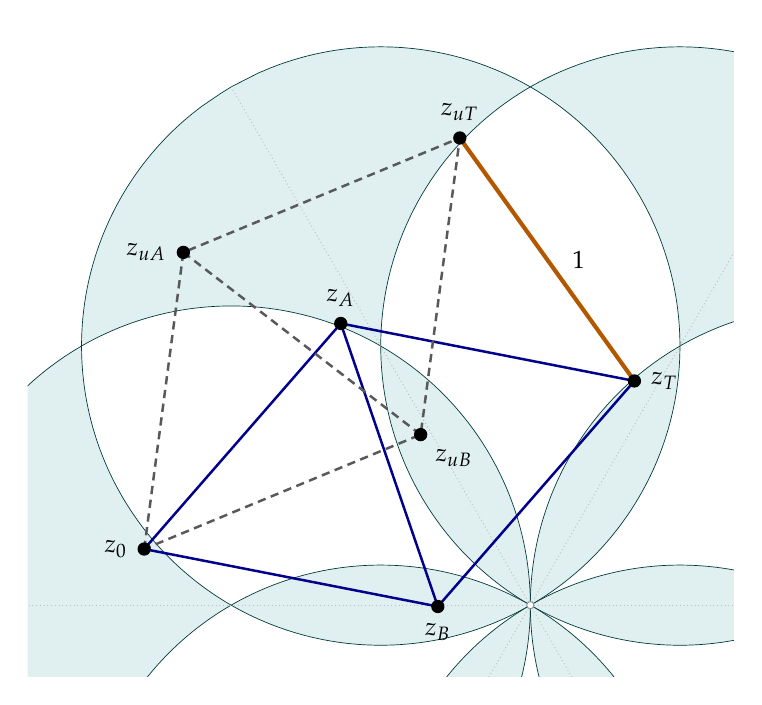
\begin{tikzpicture}[x=3.8cm,y=3.8cm,font=\small,
  vertex/.style={circle,fill=black,inner sep=1.7pt},
  first/.style={blue!55!black,line width=.9pt},
  second/.style={black!65,line width=.9pt,densely dashed}]
  \begin{scope}
    \clip (-1.68,-.24) rectangle (.68,1.93);
    \foreach \sector in {0,60,120,180,240,300} {
      \path[fill=teal!12,draw=teal!45!black,line width=.25pt]
        plot[domain=0:1,samples=101,variable=\r]
          ({\r*cos(\sector+acos(\r/2)-60)},
           {\r*sin(\sector+acos(\r/2)-60)})
        -- plot[domain=1:0,samples=101,variable=\r]
          ({\r*cos(\sector-acos(\r/2)+60)},
           {\r*sin(\sector-acos(\r/2)+60)}) -- cycle;
      \path[fill=teal!12,draw=teal!45!black,line width=.25pt]
        plot[domain=1:sqrt(3),samples=101,variable=\r]
          ({\r*cos(\sector+60-acos(\r/2))},
           {\r*sin(\sector+60-acos(\r/2))})
        -- plot[domain=sqrt(3):2,samples=101,variable=\r]
          ({\r*cos(\sector+acos(\r/2))},
           {\r*sin(\sector+acos(\r/2))})
        -- plot[domain=2:sqrt(3),samples=101,variable=\r]
          ({\r*cos(\sector-acos(\r/2))},
           {\r*sin(\sector-acos(\r/2))})
        -- plot[domain=sqrt(3):1,samples=101,variable=\r]
          ({\r*cos(\sector-60+acos(\r/2))},
           {\r*sin(\sector-60+acos(\r/2))}) -- cycle;
    }
    \foreach \sector in {0,60,120,180,240,300}
      \draw[black!25,densely dotted,line width=.35pt]
        (0,0) -- (\sector:2);
    \draw[fill=white,draw=black!45,line width=.3pt]
      (0,0) circle[radius=.012];
  \end{scope}
  \foreach \name/\gx/\gy in {
    O/0/0,
    A/{sqrt(3)/2}/{1/2},
    B/{sqrt(3)/2}/{-1/2},
    T/{sqrt(3)}/0,
    UA/{(5*sqrt(3)-sqrt(11))/12}/{(sqrt(33)+5)/12},
    UB/{(5*sqrt(3)+sqrt(11))/12}/{(sqrt(33)-5)/12},
    UT/{5*sqrt(3)/6}/{sqrt(33)/6}}
  {
    \coordinate (\name) at
      ({(35*(\gx-290/250)-12*(\gy+149/250))/37},
       {(12*(\gx-290/250)+35*(\gy+149/250))/37});
  }
  \draw[first] (O) -- (A) -- (T) -- (B) -- (O);
  \draw[first] (A) -- (B);
  \draw[second] (O) -- (UA) -- (UT) -- (UB) -- (O);
  \draw[second] (UA) -- (UB);
  \draw[orange!70!black,line width=1.5pt] (T) --
    node[midway,right=5pt,text=black] {$1$} (UT);

  \node[vertex,label=left:$z_0$] at (O) {};
  \node[vertex,label=above:$z_A$] at (A) {};
  \node[vertex,label=below:$z_B$] at (B) {};
  \node[vertex,label=right:$z_T$] at (T) {};
  \node[vertex,label=left:$z_{uA}$] at (UA) {};
  \node[vertex,label=below right:$z_{uB}$] at (UB) {};
  \node[vertex,label=above:$z_{uT}$] at (UT) {};
\end{tikzpicture}

\caption{The Moser graph in the placement $z_g$. All eleven drawn edges
have unit length. The two triangles sharing $z_Az_B$ force $z_0,z_T$
to have the same color in any proper three-coloring; the dashed diamond forces
$z_0,z_{uT}$ to have the same color. The highlighted edge $z_Tz_{uT}$
contradicts these equalities. The shading gives a cropped view of the open
region \eqref{eq:source-27}, using sampled analytic boundaries; the
boundaries and radii zero, one, and two are excluded. Dotted rays mark
the sector boundaries at multiples of \(\pi/3\).
The rational certificate in Section~\ref{sec:angular-certificate-verification}
proves strict membership of every vertex in that region, which is
restricted almost everywhere to three labels.}
\label{fig:moser-placement}
\end{figure}

The following certificate gives the strict membership needed to finish
the geometric argument.

\begin{lemma}[Seven-point certificate]\label{lem:angular-certificate}
Every \(z_g\) in \eqref{eq:angular-placement} satisfies
\(0<\abs{z_g}^2<4\) and \eqref{eq:source-27}.
\end{lemma}

The full rational verification is given in
Section~\ref{sec:angular-certificate-verification}.  We first use the
certificate to finish the geometric argument.

\begin{proposition}\label{prop:angular-three}
The extracted interface cycle cannot have length three.
\end{proposition}

\begin{proof}
Lemmas~\ref{lem:angular-region} and \ref{lem:angular-certificate}
give, for each of the seven points \(x+z_g\), an open
neighborhood restricted almost everywhere to the triangle
labels.  Choose \(\rho>0\) so that each point remains in
its corresponding neighborhood after any common translation
\(t\in B(0,\rho)\).  For each vertex, the translations
that put it outside the typical set, or in the null subset
where a nontriangle label occurs, form a null set.  The
union of these seven exceptional translation sets is null.
Choose \(t\) outside that union.  All seven translated
vertices are then typical and use the three triangle labels.
Their unit edges are preserved by the placement and common
translation, and typical-point properness gives a proper
three-coloring of the graph in
\eqref{eq:angular-seven-vectors}.  The two shared-edge
triangle pairs proved that this graph has no such coloring.
\end{proof}

\begin{proof}[Proof of Theorem~\ref{thm:weak-five}]
If a weak measurable five-coloring existed,
Proposition~\ref{prop:interface-cycle} would produce an
interface cycle of length three, four, or five with the
common-center and exclusion properties used above.
Propositions~\ref{prop:angular-five}, \ref{prop:angular-four},
and \ref{prop:angular-three} exclude all three possibilities.
Thus no weak measurable five-coloring exists.
\end{proof}

\subsection{Rational verification of the seven-point certificate}
\label{sec:angular-certificate-verification}

All terminating decimals in this verification denote exact rational
numbers.

\begin{proof}[Proof of Lemma~\ref{lem:angular-certificate}]
Table~\ref{tab:angular-coordinates} gives coordinate centers
\((\xi_0,\upsilon_0)\), each within \(h=0.00011\) of
the corresponding exact coordinate of \(z_g\), and strict
upper and lower polynomial bounds.
\begin{table}[htbp]
\centering
\begin{tabular}{@{}crrrr@{}}
\toprule
\(g\)&\(\xi_0\)&\(\upsilon_0\)&\(P_+\)&\(P'_-\)\\
\midrule
\(0\)&\(-1.2906\)&\(0.1876\)&\(0.90\)&\(1.35\)\\
\(A\)&\(-0.6335\)&\(0.9414\)&\(0.095\)&\(0.110\)\\
\(B\)&\(-0.3092\)&\(-0.0045\)&\(0.000002\)&\(0.00065\)\\
\(T\)&\(0.3478\)&\(0.7493\)&\(0.023\)&\(0.026\)\\
\(uA\)&\(-1.1598\)&\(1.1790\)&\(9.8\)&\(19.0\)\\
\(uB\)&\(-0.3666\)&\(0.5700\)&\(0.0022\)&\(0.024\)\\
\(uT\)&\(-0.2358\)&\(1.5614\)&\(12.65\)&\(12.9\)\\
\bottomrule
\end{tabular}
\caption{Coordinate boxes and bounds \(P<P_+<P'_-<P'\).}
\label{tab:angular-coordinates}
\end{table}

Here are explicit checks of the boxes and polynomial bounds.
Squaring rational endpoints proves
\[
 1.73205<\sqrt3<1.73206,\qquad
 3.31662<\sqrt{11}<3.31663.
\]
Put \(a_*=1.732055\), \(b_*=3.316625\), and
\(\epsilon=0.000005\).  Replacing the two radicals by
these midpoints changes their product by less than
\[
 (a_*+b_*)\epsilon+\epsilon^2
 =0.000025243425<0.000026.
\]
The coordinates of the three products in
\eqref{eq:angular-seven-vectors} are
\begin{align*}
 uA&=\left(\frac{5\sqrt3-\sqrt{11}}{12},
                 \frac{\sqrt{33}+5}{12}\right),\\
 uB&=\left(\frac{5\sqrt3+\sqrt{11}}{12},
                 \frac{\sqrt{33}-5}{12}\right),\\
 uT&=\left(\frac{5\sqrt3}{6},\frac{\sqrt{33}}6\right).
\end{align*}
For each coordinate of every \(g\), the midpoint substitution
therefore has error at most \(\epsilon\): the largest product
error is less than \(0.000026/6<\epsilon\), and the other
coefficients give this bound directly.  The rotation in
\eqref{eq:angular-placement} has absolute row sum \(47/37\).
For an exact check of the displayed centers, let
\(\widetilde z_g\) denote the placed point after this rational
midpoint substitution.  Direct substitution gives the residuals
\[
 \widetilde z_g-(\xi_0+i\upsilon_0)
       =\frac{d_x+i d_y}{710400000000},
 \qquad
 \begin{array}{c|rr}
 g&d_x&d_y\\\hline
 0&3840000&-23040000\\
 A&-29520000&10176000\\
 B&-12240000&-22464000\\
 T&25440000&10752000\\
 uA&32043244&-19212795\\
 uB&4763244&-27212795\\
 uT&32966488&-23385590
 \end{array}
\]
Every residual numerator has magnitude less than
\(35520000=710400000000/20000\), proving that the midpoint-substituted coordinates
have the stated four-decimal roundings, with error less than
\(0.00005\).  Thus every final coordinate error is bounded by
\[
 \frac{47}{37}\epsilon+0.00005<0.00011=h.
\]

For completeness, the remaining interval calculations reduce
to the small rational factors in Table~\ref{tab:angular-factors}.
Define
\begin{align*}
 x_l&=(\abs{\xi_0}-h)^2,&x_u&=(\abs{\xi_0}+h)^2,\\
 y_l&=(\abs{\upsilon_0}-h)^2,&y_u&=(\abs{\upsilon_0}+h)^2,\\
 l_l&=x_l+y_l,&l_u&=x_u+y_u,\\
 H&=\max(\abs{3x_l-y_u},\abs{3x_u-y_l}).
\end{align*}
All listed absolute coordinate centers exceed \(h\), so
these intervals enclose \(\xi^2,\upsilon^2,l\).
In each row the factors in the second table satisfy
\[
 y_u<b_y,\qquad H<b_H,\qquad a<l_l\le l_u<b.
\]
These claims require only squaring integers: with
\(M=10^5\), \(m=M\abs{\xi_0}\), \(n=M\abs{\upsilon_0}\),
the four squared-coordinate endpoints are
\[
 (x_l,x_u,y_l,y_u)
 =\frac1{10^{10}}
   \bigl((m-11)^2,(m+11)^2,(n-11)^2,(n+11)^2\bigr).
\]
Thus every entry is verifiable using the displayed coordinate
integers, without evaluation of an irrational number.
\begin{table}[htbp]
\centering
\begin{tabular}{@{}crrrr@{}}
\toprule
\(g\)&\(b_y\)&\(b_H\)&\(a\)&\(b\)\\
\midrule
\(0\)&\(0.0353\)&\(4.963\)&\(1.70\)&\(1.71\)\\
\(A\)&\(0.887\)&\(0.319\)&\(1.28\)&\(1.29\)\\
\(B\)&\(0.000022\)&\(0.287\)&\(0.095\)&\(0.096\)\\
\(T\)&\(0.562\)&\(0.199\)&\(0.682\)&\(0.683\)\\
\(uA\)&\(1.391\)&\(2.647\)&\(2.73\)&\(2.74\)\\
\(uB\)&\(0.326\)&\(0.079\)&\(0.459\)&\(0.46\)\\
\(uT\)&\(2.44\)&\(2.273\)&\(2.493\)&\(2.495\)\\
\bottomrule
\end{tabular}
\caption{Rational factors bounding the squared-coordinate boxes.}
\label{tab:angular-factors}
\end{table}

Every interval \((a,b)\) lies in \((0,4)\) and avoids one.
The polynomial factors are therefore bounded by
\begin{align*}
 P&\le y_u H^2<b_yb_H^2<P_+,\\
 P'&\ge l_l^3(1-l_u/4)
          \min(\abs{l_l-1},\abs{l_u-1})^2\\
   &>a^3(1-b/4)\min(\abs{a-1},\abs{b-1})^2>P'_-.
\end{align*}
The last inequalities are direct rational products of
the second table, with the target bounds in the first.
For example, its final row gives
\[
 2.44(2.273)^2<12.65,
 \qquad
 (2.493)^3(1-2.495/4)(1.493)^2>12.9.
\]
The other six rows give the corresponding displayed strict
bounds by the same two products.  The squared-radius
intervals also lie respectively in
\[
 (1.70,1.71),\ (1.28,1.29),\ (0.095,0.096),\ (0.68,0.69),
 \ (2.73,2.74),\ (0.459,0.46),\ (2.49,2.50).
\]
Finally \(P_+<P'_-\) in every row of
Table~\ref{tab:angular-coordinates}.  This proves
\eqref{eq:source-27} and the radius conditions for all seven
vertices.
\end{proof}

\begingroup
\raggedright
\setlength{\bibsep}{5pt}
\bibliographystyle{abbrvnat}
\bibliography{references}
\endgroup
\end{document}
